% Options for packages loaded elsewhere
\PassOptionsToPackage{unicode}{hyperref}
\PassOptionsToPackage{hyphens}{url}
%
\documentclass[
]{book}
\usepackage{amsmath,amssymb}
\usepackage{lmodern}
\usepackage{ifxetex,ifluatex}
\ifnum 0\ifxetex 1\fi\ifluatex 1\fi=0 % if pdftex
  \usepackage[T1]{fontenc}
  \usepackage[utf8]{inputenc}
  \usepackage{textcomp} % provide euro and other symbols
\else % if luatex or xetex
  \usepackage{unicode-math}
  \defaultfontfeatures{Scale=MatchLowercase}
  \defaultfontfeatures[\rmfamily]{Ligatures=TeX,Scale=1}
\fi
% Use upquote if available, for straight quotes in verbatim environments
\IfFileExists{upquote.sty}{\usepackage{upquote}}{}
\IfFileExists{microtype.sty}{% use microtype if available
  \usepackage[]{microtype}
  \UseMicrotypeSet[protrusion]{basicmath} % disable protrusion for tt fonts
}{}
\makeatletter
\@ifundefined{KOMAClassName}{% if non-KOMA class
  \IfFileExists{parskip.sty}{%
    \usepackage{parskip}
  }{% else
    \setlength{\parindent}{0pt}
    \setlength{\parskip}{6pt plus 2pt minus 1pt}}
}{% if KOMA class
  \KOMAoptions{parskip=half}}
\makeatother
\usepackage{xcolor}
\IfFileExists{xurl.sty}{\usepackage{xurl}}{} % add URL line breaks if available
\IfFileExists{bookmark.sty}{\usepackage{bookmark}}{\usepackage{hyperref}}
\hypersetup{
  pdftitle={A New Instrument for Microbial Epidemiology},
  pdfauthor={Matthijs S. Berends},
  hidelinks,
  pdfcreator={LaTeX via pandoc}}
\urlstyle{same} % disable monospaced font for URLs
\usepackage{color}
\usepackage{fancyvrb}
\newcommand{\VerbBar}{|}
\newcommand{\VERB}{\Verb[commandchars=\\\{\}]}
\DefineVerbatimEnvironment{Highlighting}{Verbatim}{commandchars=\\\{\}}
% Add ',fontsize=\small' for more characters per line
\usepackage{framed}
\definecolor{shadecolor}{RGB}{248,248,248}
\newenvironment{Shaded}{\begin{snugshade}}{\end{snugshade}}
\newcommand{\AlertTok}[1]{\textcolor[rgb]{0.94,0.16,0.16}{#1}}
\newcommand{\AnnotationTok}[1]{\textcolor[rgb]{0.56,0.35,0.01}{\textbf{\textit{#1}}}}
\newcommand{\AttributeTok}[1]{\textcolor[rgb]{0.77,0.63,0.00}{#1}}
\newcommand{\BaseNTok}[1]{\textcolor[rgb]{0.00,0.00,0.81}{#1}}
\newcommand{\BuiltInTok}[1]{#1}
\newcommand{\CharTok}[1]{\textcolor[rgb]{0.31,0.60,0.02}{#1}}
\newcommand{\CommentTok}[1]{\textcolor[rgb]{0.56,0.35,0.01}{\textit{#1}}}
\newcommand{\CommentVarTok}[1]{\textcolor[rgb]{0.56,0.35,0.01}{\textbf{\textit{#1}}}}
\newcommand{\ConstantTok}[1]{\textcolor[rgb]{0.00,0.00,0.00}{#1}}
\newcommand{\ControlFlowTok}[1]{\textcolor[rgb]{0.13,0.29,0.53}{\textbf{#1}}}
\newcommand{\DataTypeTok}[1]{\textcolor[rgb]{0.13,0.29,0.53}{#1}}
\newcommand{\DecValTok}[1]{\textcolor[rgb]{0.00,0.00,0.81}{#1}}
\newcommand{\DocumentationTok}[1]{\textcolor[rgb]{0.56,0.35,0.01}{\textbf{\textit{#1}}}}
\newcommand{\ErrorTok}[1]{\textcolor[rgb]{0.64,0.00,0.00}{\textbf{#1}}}
\newcommand{\ExtensionTok}[1]{#1}
\newcommand{\FloatTok}[1]{\textcolor[rgb]{0.00,0.00,0.81}{#1}}
\newcommand{\FunctionTok}[1]{\textcolor[rgb]{0.00,0.00,0.00}{#1}}
\newcommand{\ImportTok}[1]{#1}
\newcommand{\InformationTok}[1]{\textcolor[rgb]{0.56,0.35,0.01}{\textbf{\textit{#1}}}}
\newcommand{\KeywordTok}[1]{\textcolor[rgb]{0.13,0.29,0.53}{\textbf{#1}}}
\newcommand{\NormalTok}[1]{#1}
\newcommand{\OperatorTok}[1]{\textcolor[rgb]{0.81,0.36,0.00}{\textbf{#1}}}
\newcommand{\OtherTok}[1]{\textcolor[rgb]{0.56,0.35,0.01}{#1}}
\newcommand{\PreprocessorTok}[1]{\textcolor[rgb]{0.56,0.35,0.01}{\textit{#1}}}
\newcommand{\RegionMarkerTok}[1]{#1}
\newcommand{\SpecialCharTok}[1]{\textcolor[rgb]{0.00,0.00,0.00}{#1}}
\newcommand{\SpecialStringTok}[1]{\textcolor[rgb]{0.31,0.60,0.02}{#1}}
\newcommand{\StringTok}[1]{\textcolor[rgb]{0.31,0.60,0.02}{#1}}
\newcommand{\VariableTok}[1]{\textcolor[rgb]{0.00,0.00,0.00}{#1}}
\newcommand{\VerbatimStringTok}[1]{\textcolor[rgb]{0.31,0.60,0.02}{#1}}
\newcommand{\WarningTok}[1]{\textcolor[rgb]{0.56,0.35,0.01}{\textbf{\textit{#1}}}}
\usepackage{longtable,booktabs,array}
\usepackage{calc} % for calculating minipage widths
% Correct order of tables after \paragraph or \subparagraph
\usepackage{etoolbox}
\makeatletter
\patchcmd\longtable{\par}{\if@noskipsec\mbox{}\fi\par}{}{}
\makeatother
% Allow footnotes in longtable head/foot
\IfFileExists{footnotehyper.sty}{\usepackage{footnotehyper}}{\usepackage{footnote}}
\makesavenoteenv{longtable}
\usepackage{graphicx}
\makeatletter
\def\maxwidth{\ifdim\Gin@nat@width>\linewidth\linewidth\else\Gin@nat@width\fi}
\def\maxheight{\ifdim\Gin@nat@height>\textheight\textheight\else\Gin@nat@height\fi}
\makeatother
% Scale images if necessary, so that they will not overflow the page
% margins by default, and it is still possible to overwrite the defaults
% using explicit options in \includegraphics[width, height, ...]{}
\setkeys{Gin}{width=\maxwidth,height=\maxheight,keepaspectratio}
% Set default figure placement to htbp
\makeatletter
\def\fps@figure{htbp}
\makeatother
\setlength{\emergencystretch}{3em} % prevent overfull lines
\providecommand{\tightlist}{%
  \setlength{\itemsep}{0pt}\setlength{\parskip}{0pt}}
\setcounter{secnumdepth}{5}
\usepackage{booktabs}
\usepackage{amsthm}
\makeatletter
\def\thm@space@setup{%
  \thm@preskip=8pt plus 2pt minus 4pt
  \thm@postskip=\thm@preskip
}
\makeatother
\ifluatex
  \usepackage{selnolig}  % disable illegal ligatures
\fi
\usepackage[]{natbib}
\bibliographystyle{apalike}

\title{A New Instrument for Microbial Epidemiology}
\usepackage{etoolbox}
\makeatletter
\providecommand{\subtitle}[1]{% add subtitle to \maketitle
  \apptocmd{\@title}{\par {\large #1 \par}}{}{}
}
\makeatother
\subtitle{Empowering Antimicrobial Resistance Data Analysis}
\author{Matthijs S. Berends}
\date{25 August 2021}

\begin{document}
\maketitle

{
\setcounter{tocdepth}{1}
\tableofcontents
}
\hypertarget{preamble}{%
\chapter*{Preamble}\label{preamble}}
\addcontentsline{toc}{chapter}{Preamble}

This is the integral PhD thesis `A New Instrument for Microbial Epidemiology' (DOI \href{https://doi.org/10.33612/diss.177417131}{10.33612/diss.177417131}) by \href{https://www.rug.nl/staff/m.s.berends}{Matthijs S. Berends}, which was defended publicly at the University of Groningen, the Netherlands, on 25 August 2021.

All texts were copied from the printed version `as is'; no modifications were made.

\hypertarget{short-summary-250-words}{%
\subsection*{Short summary (250 words)}\label{short-summary-250-words}}
\addcontentsline{toc}{subsection}{Short summary (250 words)}

Treating infectious diseases requires insights into the microorganisms causing infectious diseases. Antimicrobial resistance (AMR) in microorganisms limits treatment possibilities and poses an enormous healthcare problem worldwide. The spread and AMR patterns of microorganisms, risk factors for infection, and preventive and control measures of infectious disease are studied within the field of Microbial Epidemiology, a cross-over field between Epidemiology and Clinical Microbiology. For analysing the spread and AMR patterns of microorganisms, however, no standardised method previously existed. This thesis showcases the development and applied use of a new instrument to analyse AMR data: the AMR package for R. From multiple viewpoints, the AMR package and its advantages are put into perspective: from a technical viewpoint, from an infection management viewpoint and from a clinical viewpoint. These combined provide a common ground for comprehending what the AMR package could yield in the field and how it can set a new empowered starting point for future applications of microbial epidemiology, in clinical and research settings alike. This thesis subsequently elaborates on these multiple viewpoints by illustrating the use of this new instrument in epidemiological research projects in the Dutch-German cross-border region to better understand the occurrence and AMR patterns of microorganisms on a (eu)regional level. In conclusion, this thesis shows the added value of a consistent data-analytical instrument to prepare and analyse AMR data in a full-region approach, that can also be used in clinical settings to obtain novel insights on AMR patterns.

\hypertarget{colophon}{%
\chapter*{Colophon}\label{colophon}}
\addcontentsline{toc}{chapter}{Colophon}

Cover design: Matthijs Berends (images used with permission)\\
Layout: Matthijs Berends\\
Printing: Gildeprint -- www.gildeprint.nl

The work described within this thesis was supported by (1) the Certe Medical Diagnostics and Advice Foundation, (2) the INTERREG V A (202085) funded project EurHealth-1Health (\url{http://www.eurhealth1health.eu}), part of a Dutch-German cross-border network supported by the European Commission, the Dutch Ministry of Health, Welfare and Sport, the Ministry of Economy, Innovation, Digitalisation and Energy of the German Federal State of North Rhine-Westphalia, and the Ministry for National and European Affairs and Regional Development of the German Federal State of Lower Saxony, (3) the European Union's Horizon 2020 Research and Innovation Programme under the Marie Skłodowska-Curie Grant Agreement 713660 (MSCA-COFUND-2015-DP ``Pronkjewail''), and (4) the European Society for Clinical Microbiology and Infectious Diseases (ESCMID) through the ESCMID Study Group for Antimicrobial Stewardship (ESGAP).

Printing of this thesis was financially supported by the Certe Medical Diagnostics and Advice Foundation. This support is greatly appreciated.

\textbf{Copyright © 2021 by Matthias Simeon Berends.} All rights reserved. Any unauthorised reprint or use of this material is prohibited. No parts of this thesis may be reproduced, stored, or transmitted in any form or by any means, without written permission of the author or, when appropriate, the publishers of the publications.

\hypertarget{contents}{%
\chapter*{Contents}\label{contents}}
\addcontentsline{toc}{chapter}{Contents}

\textbf{Section I}

\begin{enumerate}
\def\labelenumi{\arabic{enumi}.}
\item
  \textbf{General Introduction}
\item
  \textbf{Diagnostic Stewardship: Sense or Nonsense?!}\\
  Berends MS*, Luz CF*, Wouthuyzen-Bakker M, Märtson AG, Alffenaar JW, Dik JWH, Glasner C, Sinha BNM\\
  \emph{Dutch Journal of Clinical Microbiology (2018) 26;3}
\item
  \textbf{Introducing a New, Free, and Independent Method for Standardised, Reproducible and Reliable Analyses of Antimicrobial Resistance Data}\\
  Berends MS, Luz CF, Sinha BNM, Glasner C\textsuperscript{‡}, Friedrich AW\textsuperscript{‡}\\
  \emph{In preparation}
\end{enumerate}

\textbf{Section II}

\begin{enumerate}
\def\labelenumi{\arabic{enumi}.}
\setcounter{enumi}{3}
\item
  \textbf{AMR - An R Package for Working with Antimicrobial Resistance Data}\\
  Berends MS*, Luz CF*, Friedrich AW, Sinha BNM, Albers CJ, Glasner C\\
  \emph{Journal of Statistical Software (2021), ahead of print}
\item
  \textbf{Rapid Analysis of Diagnostic and Antimicrobial Patterns in R (RadaR): Interactive Open-Source Software App for Infection Management and Antimicrobial Stewardship}\\
  Luz CF, Berends MS, Dik JWH, Lokate M, Pulcini C, Glasner C, Sinha BNM\\
  \emph{Journal of Medical Internet Research (2019) 21;6, e12843}
\item
  \textbf{Better Antimicrobial Resistance Data Analysis and Reporting in Less Time}\\
  Berends MS*, Luz CF*, Zhou X, Friedrich AW, Lokate ML, Sinha BNM\textsuperscript{‡}, Glasner C\textsuperscript{‡}\\
  \emph{medRxiv {[}preprint{]} (2021), 21257599}
\end{enumerate}

\textbf{Section III}

\begin{enumerate}
\def\labelenumi{\arabic{enumi}.}
\setcounter{enumi}{6}
\item
  \textbf{Trends in Occurrence and Phenotypic Resistance of Coagulase-Negative Staphylococci (CoNS) Found in Blood in the Northern Netherlands between 2013 and 2019}\\
  Berends MS, Luz CF, Ott A, Andriesse GI, Becker K, Glasner C\textsuperscript{‡}, Friedrich AW\textsuperscript{‡}\\
  \emph{In preparation}
\item
  \textbf{Defining Multidrug Resistance of Gram-Negative Bacteria in the Dutch-German Border Region-Impact of National Guidelines}\\
  Köck R, Siemer P, Esser J, Kampmeier S, Berends MS, Glasner C, Arends JP, Becker K, Friedrich AW\\
  \emph{Microorganisms (2018) 6;1}
\item
  \textbf{Changing Epidemiology of Methicillin-Resistant \emph{Staphylococcus aureus} in 42 Hospitals in the Dutch-German Border Region, 2012 to 2016: Results of the Search-and-Follow-Policy}\\
  Jurke A, Daniels-Haardt I, Silvis W, Berends MS, Glasner C, Becker K, Köck R, Friedrich AW\\
  \emph{Eurosurveillance (2019) 24;15}
\item
  \textbf{A Prospective Multicentre MDRO Screening Study on ICUs in the Dutch-German Cross-Border Region (2017-2018): The Importance of Healthcare Structures}\\
  Berends MS*, Glasner C*, Becker K, Esser J, Gieffers J, Jurke A, Kampinga G, Kampmeier S, Klont R, Köck R, Al Naemi N, Ott A, Ruis G, Saris K, Tami A, Van Zeijl J, Von Müller L, Voss A, Waar K, Friedrich AW\\
  \emph{Eurosurveillance (2021), ahead of print}
\end{enumerate}

\textbf{Section IV}

\begin{enumerate}
\def\labelenumi{\arabic{enumi}.}
\setcounter{enumi}{10}
\tightlist
\item
  \textbf{Summary and Future Perspectives}
\end{enumerate}

\textbf{Gearfetting} yn Frysk\\
\textbf{Samenvatting} in het Nederlands\\
\textbf{Zusammenfassung} auf Deutsch\\
\textbf{Alphabetical list of published work}\\
\textbf{Alphabetical list of related presentations}\\
\textbf{Acknowledgements} / Tankwurd / Dankwoord / Danksagung\\
\textbf{Curriculum Vitae}

\begin{center}\rule{0.5\linewidth}{0.5pt}\end{center}

* Equal contribution\\
\textsuperscript{‡} Equal contribution

\hypertarget{ch01-introduction}{%
\chapter{General Introduction}\label{ch01-introduction}}

\hypertarget{microbial-epidemiology}{%
\section{Microbial epidemiology}\label{microbial-epidemiology}}

Epidemiology is the medical scientific field that investigates all the factors that determine the presence or absence of diseases and disorders. While many subspecialties within this field exist nowadays, such as veterinary epidemiology and cardiovascular epidemiology, its development started with an infectious disease. Between 1846 and 1860, the world endured the third cholera pandemic, taking assumably millions of lives \textsuperscript{{[}1{]}}. The year 1854 was considered the worst year, when 23,000 people died in the United Kingdom, out of 16 million inhabitants (0.14\%) \textsuperscript{{[}2{]}}. As a side note, this is still quite less than the 146,000 UK deaths due to COVID-19 out of 56 million inhabitants (0.26\%) until March 2021 \textsuperscript{{[}3{]}}. But 1854 was also the year that the basis was laid for the field of epidemiology by John Snow, an English physician and hygiene specialist.

At the time of a local cholera outbreak at the Broad Street in London in that year, Snow did not know the exact source of cholera and called it `cholera poison' in a book he published in 1856 \textsuperscript{{[}4{]}}. Interestingly, the Italian Filippo Pacini managed to isolate the bacterium causing cholera, \emph{Vibrio cholerae}, in 1854 -- the same year that Snow investigated the outbreak \textsuperscript{{[}5{]}}. Although it was not until 1884 that \emph{V. cholerae} was formally given its name by the German Robert Koch \textsuperscript{{[}6{]}}.

In his book about the `cholera poison' , Snow famously wrote \textsuperscript{{[}4{]}}:

\begin{quote}
There is no doubt that the mortality was much diminished, as I said before, by the flight of the population, which commenced soon after the outbreak; but the attacks had so far diminished before the use of the water was stopped, that it is impossible to decide whether the well still contained the cholera poison in an active state, or whether, from some cause, the water had become free from it.
\end{quote}

For this reason, Snow hypothesised that the local outbreak was caused by poisoned water coming from a water pump. To investigate the number of cases, he drew one of the most well-known data visualisations in epidemiology, Figure \ref{fig:fig1-1} (top). In this then-novel form of data visualisation, he counted the cases per household and denoted them as stacked rectangles. This resulted in his conclusion that there had been no particular outbreak or prevalence of cholera in that part of London except among the persons who were in the habit of drinking the water of one specific water pump: the one on Broad Street. The handle of the pump was removed on the day following his briefing to the local government, leading to an end of the outbreak.

With the advancements in information technology, heatmaps would nowadays be a more effective way to visualise geographic trends, Figure \ref{fig:fig1-1} (bottom). Using modern map data as illustrated, the incredible accuracy of Snow's drawing of London from 167 years ago is also highlighted. The type of investigating geographic trends in health and disease is nowadays known as \emph{spatial} epidemiology.

\begin{figure}

{\centering 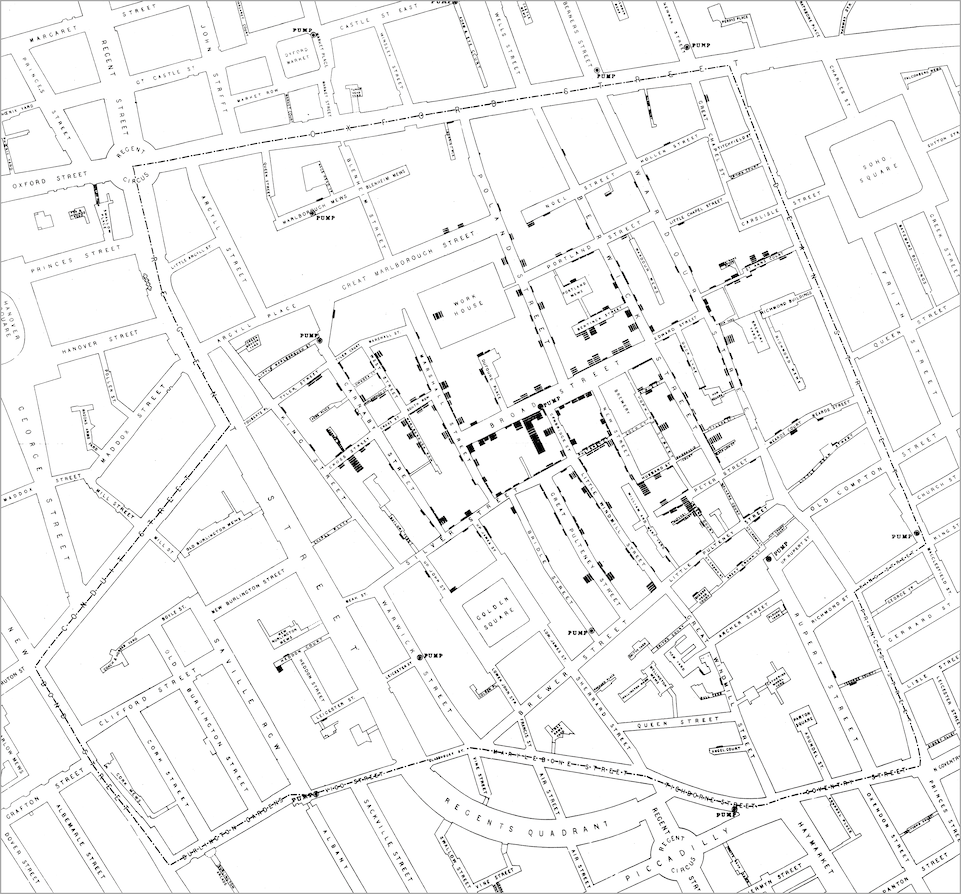
\includegraphics[width=0.8\linewidth]{images/01-01a} 

}

\end{figure}
\begin{figure}

{\centering 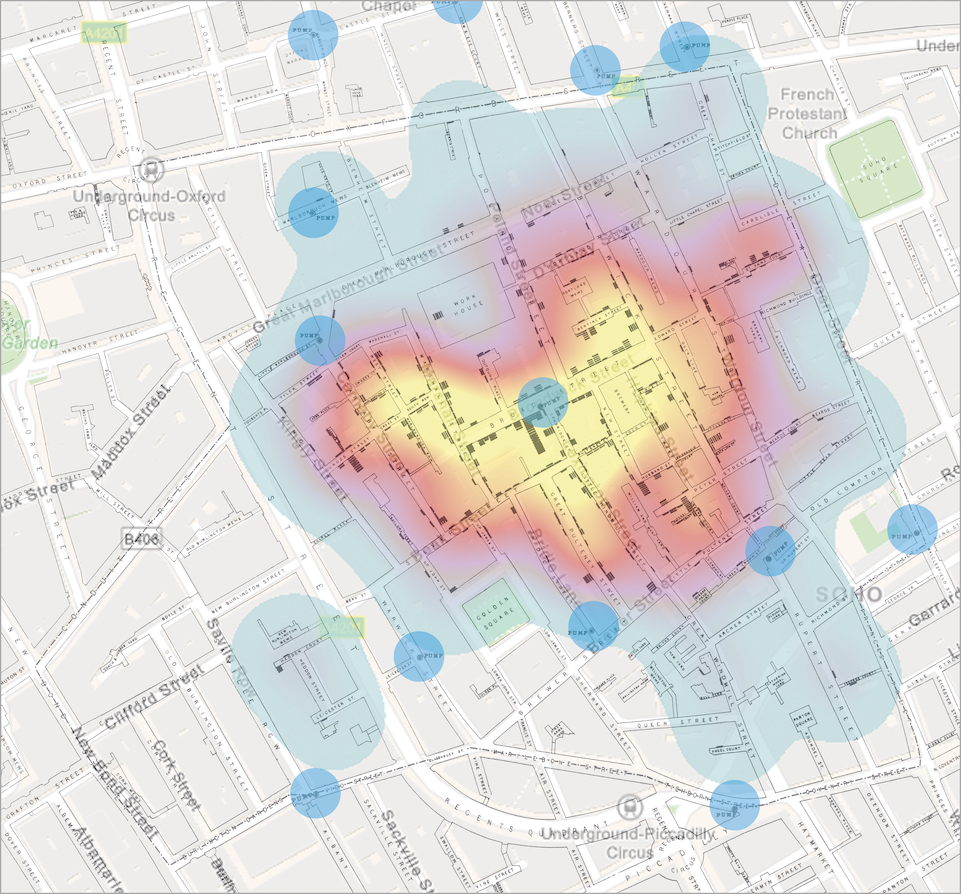
\includegraphics[width=0.8\linewidth]{images/01-01b} 

}

\caption{Visualisations of the ‘Broad Street cholera outbreak’ in London in 1854. Top: original map as drawn by John Snow. Bottom: Snow’s original map with a self-made heatmap visualisation overlay, based on the geographic position of the cases. The blue circles (n = 13) indicate the location of the water pumps.}\label{fig:fig1-1}
\end{figure}

Spatial epidemiology is one example of the many different specialities in the field of epidemiology. Another example is the direct consequence of Snow's work: infectious disease epidemiology, which has developed widely since the nineteenth century and has become the de facto standard for researching diseases and their health effects caused by pathogens (i.e., bacteria, viruses and fungi). Since this speciality concerns pathogens, it is a domain shared by the fields of epidemiology and clinical microbiology (Figure \ref{fig:fig1-2}). Moreover, infectious disease epidemiology can be split into two subspecialties: clinical (infectious disease) epidemiology and microbial epidemiology. The former focuses on the properties of the disease (such as the burden of disease caused by infection, or the disease-related mental and financial costs), while the latter focuses on the properties of the pathogen (such as the credibility of its source, antimicrobial resistance and pathogenicity).

Applying microbial epidemiology was barely possible in the days of John Snow, for the lack of scientific knowledge about pathogens and the lack of advancement in information technology. Antibiotics were not discovered yet, the cause of cholera was undetermined, and scientists had no clue about the infectivity and pathogenicity of different bacteria. However, what John Snow did in 1854 `clinical epidemiologically', is in essence quite equal to what we currently do on a large scale during the COVID-19 pandemic. Information technology required to attain this large scale has brought us not only the possibilities to look beyond regional, national and international borders but to observe, analyse and understand pandemics in real-time. Methods we develop and use today can be implemented on the other side of the world tomorrow. This is an important advantage in modern infectious disease epidemiology, as is also illustrated in this thesis.

Microbial epidemiology has an important focus on observing and analysing (1) the microorganisms that cause infections and the human site of origin, (2) the intrinsic or acquired antimicrobial resistance they manifest, and (3) their infectivity and pathogenicity. As any type of microorganism -- bacteria, viruses and fungi (including yeasts) -- can cause infections in humans, microbial epidemiology is not limited to a certain type of microorganism. Nonetheless, there tends to be a stronger focus on bacteria and fungi, which are more easily isolated at a clinical microbiology laboratory than viruses and can be tested for phenotypical antimicrobial resistance in a routine diagnostic setting. Based on these diagnostic findings, treatment guidelines are developed and evaluated. This in itself urges microbial epidemiology to be employed in a routine setting as well, to make sure that treatment guideline development continually has a solid epidemiological basis.

\begin{figure}

{\centering 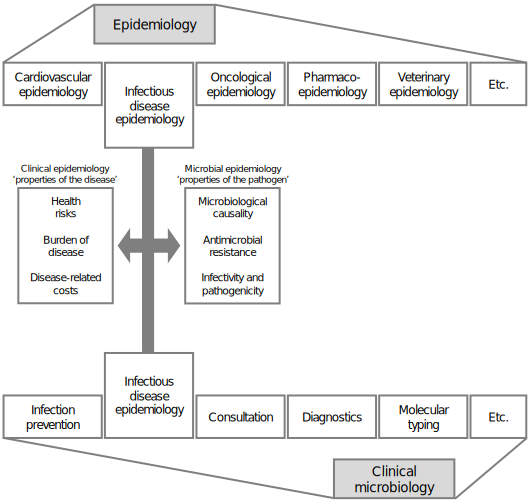
\includegraphics[width=1\linewidth]{images/01-02} 

}

\caption{Overview of the diverse sections and subspecialties of epidemiology and clinical microbiology and their common field: infectious disease epidemiology. Microbial epidemiology can be considered to be a subspecialty of infectious disease epidemiology.}\label{fig:fig1-2}
\end{figure}

\hypertarget{antimicrobial-resistance-in-microorganisms}{%
\section{Antimicrobial resistance in microorganisms}\label{antimicrobial-resistance-in-microorganisms}}

The antimicrobial resistance (AMR) that manifests in bacteria and fungi, is central within the diverse field of microbial epidemiology. It occurs when microorganisms develop mechanisms that protect them from the effects of antimicrobial agents, such as antibiotics \textsuperscript{{[}7{]}}. AMR occurring specifically in bacteria is often termed antibiotic resistance (ABR). An important distinction should be made between intrinsic AMR (that is, AMR inherently present in certain microbial species as a distinctive property of that species) and acquired AMR (that is, AMR present in some strains of a certain microbial species induced by the presence of an antimicrobial agent). Infections caused by microorganisms that are resistant to one or more antimicrobial agents cannot be treated with those antimicrobial agents anymore.

AMR is a global health problem and of great concern for human medicine, veterinary medicine, and the environment alike. It is associated with significant burdens to both patients and health care systems. Current estimates show the immense dimensions we are already facing, such as claiming at least 50,000 lives due to AMR each year across Europe and the US alone \textsuperscript{{[}8{]}}. Although estimates for the burden through AMR and their predictions are disputed by some, the rising trend is undeniable, thus calling for worldwide efforts to tackle this problem \textsuperscript{{[}9,10{]}}. For this reason, laboratory diagnostics are of utmost importance for generating AMR results that can be used to acquire new or improved AMR insights by conducting microbial epidemiology.

\hypertarget{laboratory-diagnostics}{%
\subsection{Laboratory diagnostics}\label{laboratory-diagnostics}}

From clinical illness alone (such as fever, redness, swelling, pain, and loss of function), it is impossible to determine whether the microorganism causing the infection is drug-resistant; it requires laboratory diagnostics to measure AMR. For decades, clinical microbiological laboratories have been using techniques where a defined amount of a microbial isolate is brought unto the medium of an agar plate \textsuperscript{{[}11{]}}. This technique is called the `disk diffusion test' and was first used by Dutch botanist Martinus Beijerinck in 1889 to study the effect of auxins (a class of plant hormones) on bacterial growth \textsuperscript{{[}11,12{]}}. The technique has been further developed and refined by the American microbiologists William Kirby and Alfred Bauer in 1959 and 1966, leading to this test technique sometimes being referred to as the `Kirby-Bauer test' or `KB test' \textsuperscript{{[}13,14{]}}. To perform the test, small filter paper disks containing a specified concentration of different antimicrobial agents are laid on the agar medium containing the microorganism, which is subsequently incubated for 18 to 24 hours at a specified temperature. During the incubation, the antimicrobial agent (antibiotic or antifungal) will radially diffuse over the agar, leading to high antimicrobial concentrations near the disk and low antimicrobial concentrations away from the disk. A disk typically has a diameter of 6 millimetres. After the incubation, the growth inhibition zone around the disk can be measured with a ruler. The wider the growth inhibition zone, the lower antimicrobial concentrations are required for the microorganism to inhibit growth. The narrower the growth inhibition zone, the higher antimicrobial concentrations are required for the microorganism to inhibit growth. The range of a disk diffusion test result is typically 6 to 50 millimetres.

Although disk diffusion tests is being widely used in many areas, some laboratories have replaced them with an automated incubator allowing colourimetric detection of CO2 produced by growing microorganisms in the presence of antimicrobial agents \textsuperscript{{[}15--17{]}}. Growth is subsequently optically measured for different concentrations and different antimicrobial agents. The concentration that inhibits at least 99.99\% growth of the microorganism, is denoted the minimum inhibitory concentration (MIC) and is typically expressed in milligrams per litre (mg/L). These incubators are referred to as antimicrobial susceptibility testing (AST) devices. AST devices allow for timely and reproducible results. Yet, the cartridges used for this type of instrument have a limited number of wells to test different manufacturer-set concentrations and types of antimicrobial agents. Since this limitation thus disallows testing for any desired concentration, MICs are often capped at a minimum or maximum value. For example, an actual MIC could be 128 mg/L, although the highest available concentration on a cartridge could be 32 mg/L. In such cases, the MIC will be reported as ≥ 32 mg/L. This is a technical limitation of colourimetric detection of CO2 production as a test technique, which brings important disadvantages for microbial epidemiological analyses. Capped values (such as ≤ 0.0125 mg/L and ≥ 32 mg/L) hinder comparison with previous findings or findings from other laboratories as they might conceal the true MICs. Furthermore, different cartridges may be used for bacteria isolated from different specimen types (such as urine or blood), which can yield different ranges of the resulting MICs. For example, an isolate of Staphylococcus aureus from a urinary tract infection could be tested for many concentrations of only a few orally available antibiotics using cartridge A, while an isolate of S. aureus from a complex surgical wound could be tested for only a few concentrations of many intravenously available antibiotics using cartridge B. Consequently, the MIC of e.g., ciprofloxacin could be reported as ≤ 0.0625 mg/L using cartridge A, while it could be reported as ≤ 0.125 mg/L using cartridge B, even when the S. aureus isolates are identical. This makes it hard to compare results in epidemiological data analyses as the data availability can (unknowingly) be unequal, potentially affecting the outcome of any AMR data analysis.

\hypertarget{interpretation-of-raw-results}{%
\subsection{Interpretation of raw results}\label{interpretation-of-raw-results}}

When raw AMR testing results are available, they are not yet suitable for reporting back to clinicians. The growth inhibition zones of disk diffusion tests and the MICs from the colourimetric detection tests need interpretation to consider an antimicrobial agent suitable for treatment. Typically, AMR is interpreted and reported as either (a tri-form abbreviated as `RSI'):

\begin{itemize}
\item
  R = resistant. A microorganism is categorised as `resistant' when there is a high likelihood of therapeutic failure even when there is increased exposure.\\
  Exposure is a function of how the mode of administration, dose, dosing interval, infusion time, as well as distribution and excretion of the antimicrobial agent will influence the infecting organism at the site of infection.
\item
  S = susceptible. A microorganism is categorised as `susceptible' when there is a high likelihood of therapeutic success using a standard dosing regimen of the agent.
\item
  I\\
  (according to CLSI) I = intermediate. A microorganism is categorised as `intermediate' when there is an unsure likelihood of therapeutic success. Additionally, CLSI considers a susceptible dose-dependent (SDD) category for certain drug and organism combinations, for which the susceptibility of an isolate depends on the dosing regimen used.\\
  (according to EUCAST) I = Susceptible, increased exposure. A microorganism is categorised as such when there is a high likelihood of therapeutic success because exposure to the agent is increased by adjusting the dosing regimen or by its concentration at the site of infection.
\end{itemize}

For this interpretation of raw AMR test results, international guidelines exist. The most often applied guidelines are supplied by the Clinical and Laboratory Standards Institute (CLSI) and the European Committee on Antimicrobial Susceptibility Testing (EUCAST) \textsuperscript{{[}18,19{]}}. In Europe, an increasing number of clinical laboratories apply EUCAST guidelines, as it was shown that the coverage of EUCAST guidelines among these laboratories was 73.2\% in 2013, and only a few European countries did not use the EUCAST methodology in 2019 \textsuperscript{{[}20,21{]}}. According to the World Health Organisation (WHO), guidelines from CLSI and EUCAST are adopted by 94\% of all countries reporting AMR to the Global Antimicrobial Resistance Surveillance System (GLASS) of the WHO \textsuperscript{{[}22{]}}.

Generally, AMR is defined as the proportion of resistant microorganisms (R) among all tested microorganisms of the same species (R + S + I). The CLSI and EUCAST guidelines define the interpretations for the most common combinations of pathogenic microorganisms and antimicrobial agents. For example, the EUCAST 2021 guideline considers ciprofloxacin against Escherichia coli to be susceptible when either the MIC is at most 0.25 mg/L or when a diffusion disk with 5 µg has a growth inhibition zone of at least 25 millimetres (Figure \ref{fig:fig1-3}).

In 2017, EUCAST implemented the area of technical uncertainty (ATU) for certain microbial species/antibiotic combinations, to warn laboratory staff that the interpretation of routine susceptibility testing is uncertain \textsuperscript{{[}23{]}}. For example, disk diffusion results from the combination of any species in the order of Enterobacterales with amoxicillin/clavulanic acid are considered unreliable for a zone diameter of 19-20 mm in the latest EUCAST interpretation guideline \textsuperscript{{[}24{]}}. EUCAST advises to rerun the test, perform an additional test, or to report this uncertainty with a clear warning \textsuperscript{{[}23{]}}.

\begin{figure}

{\centering 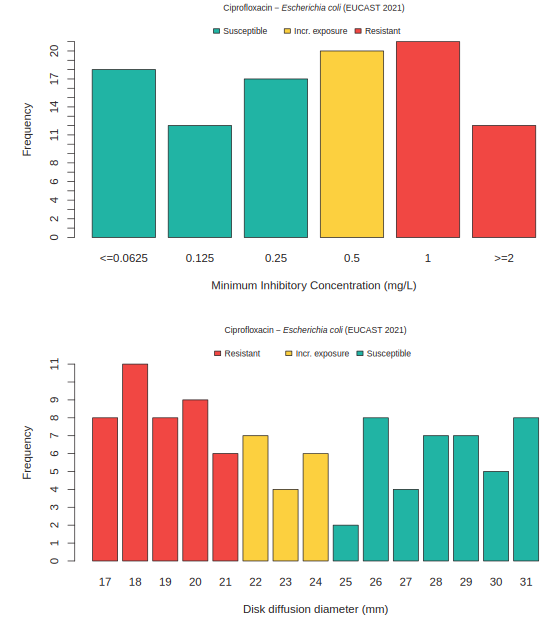
\includegraphics[width=1\linewidth]{images/01-03} 

}

\caption{Interpretation of 100 random minimum inhibitory concentrations (top) and 100 random disk diffusion growth inhibition zones (bottom) of ciprofloxacin in *Escherichia coli*, interpreted using colours according to the EUCAST 2021 guideline. These plots were generated with the AMR package for R.}\label{fig:fig1-3}
\end{figure}

To mitigate the risks of laboratories reporting erroneous susceptibility results, CLSI and EUCAST guidelines are also provided as ``expert rules'' in the previously mentioned AST devices, which helps to ensure compliance with guidelines and standards, increasing the quality of AMR data \textsuperscript{{[}25{]}}.

Analysing AMR data, such as raw MICs and antimicrobial interpretations (`RSI'), is tedious and complex, especially when evaluating cumulative AMR reports \textsuperscript{{[}26{]}}. Nonetheless, it is essential to monitor up-and-coming AMR trends at the local and regional level to support clinical decision-making, infection control interventions, and AMR containment strategies \textsuperscript{{[}27,28{]}}. AMR data analysis has been challenged by poor comparability of antimicrobial susceptibility statistics between institutions because of the diversity of calculation methods \textsuperscript{{[}26{]}}. Moreover, many laboratories have used simplistic calculation approaches, with a strong tendency to overestimate drug resistance rates \textsuperscript{{[}26{]}}. In the first ten years of this century, it was shown that this was primarily attributed to the lack of correction for duplicate isolates \textsuperscript{{[}29--31{]}}.

In an attempt to overcome this, CLSI started in 2002 with developing guidelines to recommend epidemiologically sound workflows for the analysis and presentation of AMR results and trends, with their fourth and currently latest version released in 2014 \textsuperscript{{[}32{]}}. These guidelines comprise advice on the inclusion of a minimum number of isolates, the choice of antimicrobial agents to analyse, and the presenting of numbers and percentages of AMR. In 2007, Hindler \emph{et al.} evaluated the then-latest version of this guideline \textsuperscript{{[}26{]}}. They concluded that although CLSI provided a comprehensive collection of suggestions, only a few publications had implemented these practical recommendations. Nevertheless, it continuously provides a theoretical basis for microbial epidemiological analyses but lacks suggestions of how these theoretical recommendations can be implemented practically or what kind of software would be suitable to analyse AMR data and, more specific, AMR data about multi-drug resistant organisms.

\hypertarget{multi-drug-resistant-organisms}{%
\subsection{Multi-drug resistant organisms}\label{multi-drug-resistant-organisms}}

Multi-drug resistant organisms (MDROs) are microorganisms that acquired AMR to at least one antimicrobial agent in multiple antimicrobial categories. Because of MDROs, there are countries in many parts of the world where antimicrobial treatment is ineffective in more than half of all patients \textsuperscript{{[}33{]}}. Common MDROs include vancomycin-resistant enterococci (VRE), methicillin-resistant \emph{Staphylococcus aureus} (MRSA), extended-spectrum β-lactamase (ESBL) producing Gram-negative bacteria such as \emph{E. coli} and \emph{Klebsiella pneumoniae}, carbapenemase-producing Gram-negative bacteria, third-generation cephalosporin (3GC) resistant Gram-negative bacteria and carbapenemase-producing Gram-negative bacteria.

In 2012, MDROs were formally categorised into different degrees of severity in favour of international comparison purposes \textsuperscript{{[}34{]}}. Multi-drug resistance (MDR) was defined as acquired AMR to three or more antimicrobial categories, extensive drug resistance (XDR) was defined as acquired AMR to all antimicrobial agents except in two or fewer antimicrobial categories, and pan-drug resistance (PDR) was defined as acquired AMR to all antimicrobial agents in all antimicrobial categories \textsuperscript{{[}34{]}}. MDR among microorganisms is very common, PDR is very uncommon \textsuperscript{{[}7,33,35{]}}. In 2014, the WHO published a report in which they performed five systematic reviews involving 221 studies with a special focus on MDR bacteria (defined as MRSA, 3GC/fluoroquinolone-resistant E. coli, and 3GC/carbapenem-resistant K. pneumoniae) \textsuperscript{{[}36{]}}. The outcomes of this report underlined the increasing necessity of surveillance programs.

\hypertarget{surveillance-programs}{%
\subsection{Surveillance programs}\label{surveillance-programs}}

With the current WHO surveillance program GLASS, the overall coverage of AMR is continuously being monitored for most countries of the world \textsuperscript{{[}37{]}}. For Europe, the prevalence of AMR on the country level is monitored by national surveillance programs that share their data with the European Centre for Disease Prevention and Control (ECDC), an agency of the European Union \textsuperscript{{[}38{]}}. Their surveillance program European Antimicrobial Resistance Surveillance Network (EARS-Net) is the largest publicly funded system for AMR surveillance in Europe. Public access to descriptive data (maps, graphs and tables) are available through the ECDC Surveillance Atlas of Infectious Diseases \textsuperscript{{[}38{]}}, which was also consulted for multiple studies in this thesis. While the ECDC estimated in 2009 that bacterial infections caused by MDROs were responsible for 25,000 extra deaths per year \textsuperscript{{[}39{]}}, others found that there is a large discrepancy between the real count of deaths attributable to MDROs and the subsequent alarmist predictions, based on data from over 500 studies \textsuperscript{{[}35{]}}.

Although surveillance programs allow for signalling significant differences and shifts in AMR rates, additional AMR data analyses and AMR surveillance studies are strict requirements to fully understand the continuous development in AMR rates as there is no ``ideal'' surveillance system covering all aspects \textsuperscript{{[}28{]}}. Nonetheless, the desire to continuously monitor, analyse, model and predict AMR, has led to the increased development and use of local, regional, national and international surveillance systems \textsuperscript{{[}27{]}}. Critchley \emph{et al.} have inventoried the requirement set by different types of users (Table 1).

On the local level, clinical microbiology laboratories should communicate AMR surveillance data to healthcare providers in an understandable manner. Since MDROs can migrate between healthcare institutions, countries and continents by migrating people, local healthcare providers should be aware of local, regional, national and international surveillance program implementations and their ensuing results on AMR. On the other hand, such surveillance program implementations should be well-designed, well-maintained, longitudinal, and involve an appropriate collaboration with local laboratories over time \textsuperscript{{[}27{]}}.

Table 1. Uses of antibiotic resistance surveillance system data by hospitals, university researchers, pharmaceutical companies and governments. From Critchley \emph{et al.}, 2004 \textsuperscript{{[}27{]}}.

\begin{figure}

{\centering 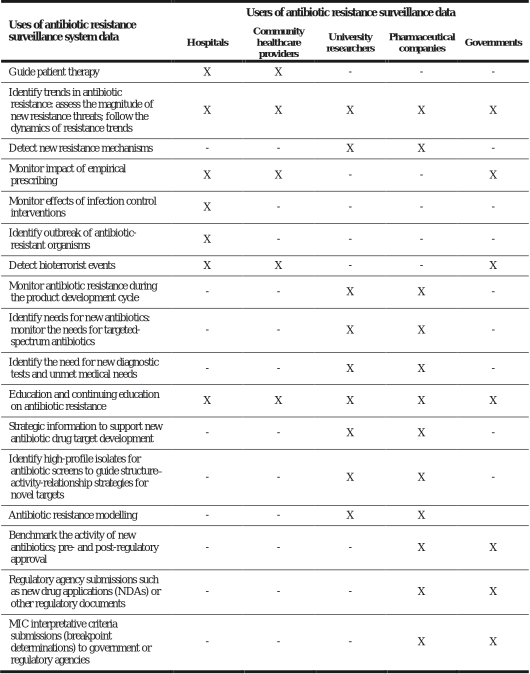
\includegraphics[width=1\linewidth]{images/01-t01} 

}

\end{figure}

As an example, ISIS-AR (Infectious disease Surveillance Information System for Antibiotic Resistance) is a Dutch national surveillance program, for which a large number of the Dutch clinical microbiology laboratories provide anonymised data on AMR to the National Institute for Public Health and the Environment (Rijksinstituut voor Volksgezondheid en Milieu, RIVM) \textsuperscript{{[}40{]}}. In Germany, ARS (Antibiotic Resistance Surveillance) is a similar laboratory-based national surveillance program, that attempts to enable differential statements according to structural characteristics of health care and regions \textsuperscript{{[}41,42{]}}. Both these national surveillance programs provide data for EARS-Net and GLASS of the WHO \textsuperscript{{[}37,43{]}}.

\hypertarget{data-analysis-using-r}{%
\section{Data analysis using R}\label{data-analysis-using-r}}

In academia, the free and open-source statistical language R is an increasingly popular tool for analysing study results and developing new scientific methods, especially in medical fields such as human genetics, health decision sciences, and proteomics \textsuperscript{{[}44--47{]}}. Even more so, a new type of study seems to currently arise where researchers from different medical fields publish tutorials on how to acquire new insights using R as a programming language \textsuperscript{{[}48--50{]}}. In 2020, R ranked 8th in the TIOBE index, a global initiative to measure the popularity of programming languages, while it ranked 73rd in 2008 \textsuperscript{{[}51{]}}.

R was developed for statistical computing and graphics supported by the R Foundation for Statistical Computing \textsuperscript{{[}52,53{]}}. It is freely available under the GNU General Public License v2, meaning that it may be used for both private and commercial purposes in any way, but not for patent purposes. As a statistical package, it is comparable to the proprietary software programs Stata, SAS and SPSS \textsuperscript{{[}54{]}}. However, as opposed to these proprietary software programs, R has an open file format and can read data from any source, including files from other software programs, and websites. Moreover, the `base' functions of R are extendible by users who develop so-called packages for R. The Comprehensive R Archive Network (CRAN) that hosts and maintains R through the R Foundation for Statistical Computing, accepts package submissions from users and subjects users to a peer-review submission process and a strict repository policy \textsuperscript{{[}53,55{]}}. As of May 2021, the CRAN package repository features 17,671 available packages.

Not only the popularity of using R has increased over the last decade. The number of developed packages has also increased strongly over the last years, especially since 2016 (Figure \ref{fig:fig1-4}). This is probably attributed to a rather new integrated desktop environment (IDE) to use R, called RStudio \textsuperscript{{[}56{]}}. RStudio is also the name of the corporation that developed the RStudio IDE and authored the so-called tidyverse, a collection of R packages (such as dplyr and ggplot2) that are specifically designed to ease data importing, tidying, manipulating, visualising, and programming, as well as to improve code reading \textsuperscript{{[}57--59{]}}. The tidyverse can be used for most data analytical tasks and has been the method of choice for numerous (clinical) studies, including those presented in this thesis.

\begin{figure}

{\centering 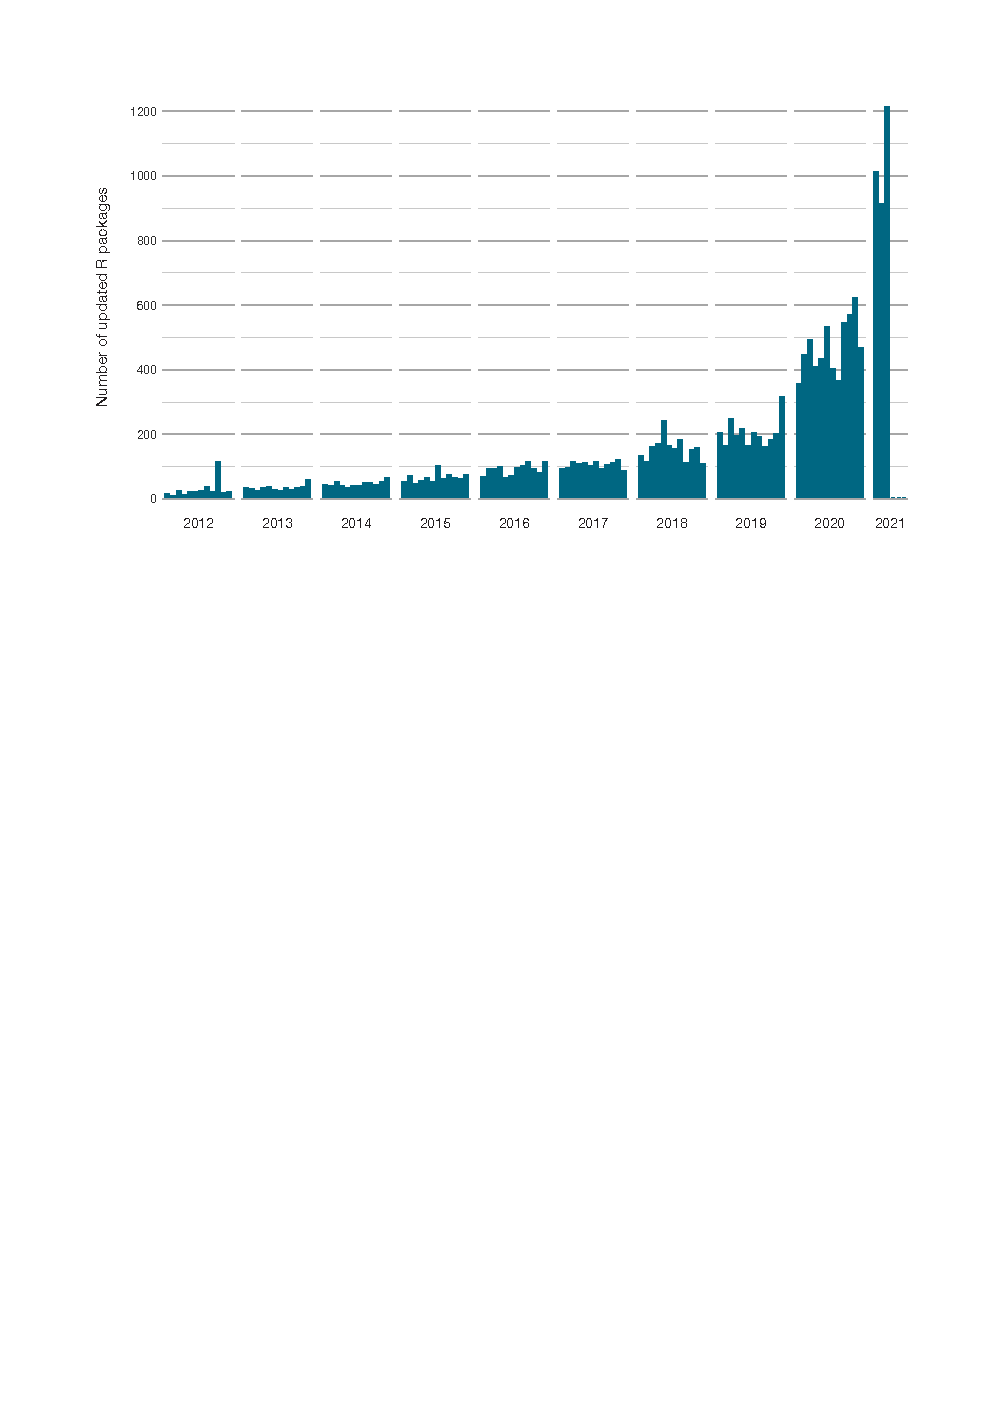
\includegraphics[width=1\linewidth]{images/01-04} 

}

\caption{The number of R packages by date of the last update over the last ten years. Every bar represents one month. Every R package occurs once in this figure.}\label{fig:fig1-4}
\end{figure}

For microbial epidemiology, no particular R packages were available to analyse phenotypic AMR test results as of 2017. One R package that provides approaches to work with disk diffusion zone diameters and MICs from environment samples started development in 2018, but still has no released version as of May 2021 \textsuperscript{{[}60{]}}. For `non-microbial' infectious disease epidemiology, however, outbreaks and epidemics could already be analysed with dedicated packages in R \textsuperscript{{[}61--65{]}}. Most of these packages were developed within RECON, the R Epidemics Consortium, that gathers experts in data science, modelling methodology, public health, and software development to create the next generation of analytics tools in R for informing the response to disease outbreaks, health emergencies and humanitarian crises. Their R package EpiEstim is being used worldwide for calculating and presenting reproduction rates of SARS-CoV-2 during the ongoing COVID-19 pandemic, also by the Dutch National Institute for Public Health and the Environment (RIVM) \textsuperscript{{[}65,66{]}}.

\hypertarget{setting-for-this-thesis}{%
\section{Setting for this thesis}\label{setting-for-this-thesis}}

Studies within this thesis were geographically organised or initiated in the Northern cross-border region of the Netherlands and Germany, Figure \ref{fig:fig1-5}. According to the German philosopher Liessmann, there are only national borders defined by humans, but no natural borders \textsuperscript{{[}67{]}}. He explained that borders as man-made conventions are never absolute, but that it is always possible to cross them. Despite the existing territorial border, there are many similarities in the Netherlands and Germany today, but just as many and clear differences, especially concerning the healthcare sector. A German patient can become a patient in the Netherlands just as quickly as a Dutch patient can in Germany. Since pathogens know no borders, patient protection and infection prevention must not stop at borders \textsuperscript{{[}68{]}}. The Netherlands and Germany have, among many other matters, apparent differences within the healthcare system in general and in terms of AMR, especially concerning MDRO definitions and infection prevention guidelines. To study these differences, INTERREG programs enable cross-border, transnational and interregional cooperation. INTERREG is one of the central instruments in European cohesion and regional policy, with which the development differences between the European countries in the border regions should be reduced and economic cohesion strengthened. It aims to ensure that national borders are not an obstacle to the balanced development and integration of the European territory \textsuperscript{{[}69{]}}. One of its programs, EurHealth-1Health, was a large research project that aimed to facilitate working together in battling AMR and MDROs and to empower sustainable collaborations across the border.

\begin{figure}

{\centering 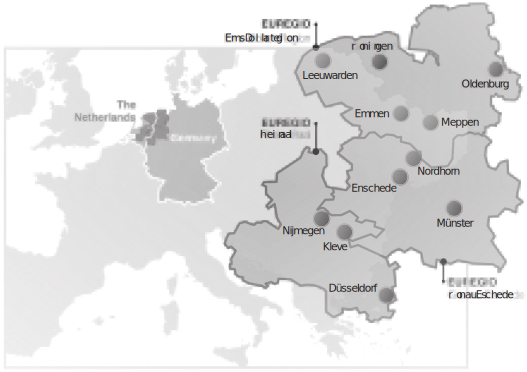
\includegraphics[width=1\linewidth]{images/01-05} 

}

\caption{Geographic overview of three Euregio’s that make up most of the Dutch-German cross-border region.}\label{fig:fig1-5}
\end{figure}

In the Northern Netherlands, five clinical microbiological laboratories together conduct the microbiological diagnostics for more than two million Dutch inhabitants in primary care, secondary care (non-university hospitals) and tertiary care (university hospital). Three of these five are regional non-profit laboratories: Izore in Leeuwarden (Friesland), Certe in Groningen (Groningen) and LabMicTA in Hengelo (Overijssel). The other two laboratories are hospital departments of the Isala hospital in Zwolle (Overijssel) and the University Medical Center Groningen. On the other side of the border in Germany, laboratories are more numerous, more centralised, often privatised, and organised on a different scale than in the Netherlands. This is largely due to a higher number of small hospitals in Germany compared to the Netherlands, which is inherent to the different healthcare structures. In 2018, Germany had 2.33 hospitals per 100,000 inhabitants (1 hospital per 43,010 inhabitants), while in the Netherlands this was 0.68 hospitals per 100,000 inhabitants (1 hospital per 148,113 inhabitants), almost 3.5 times less \textsuperscript{{[}70--73{]}}.

These differences posed important reasons to research the effects of having different national guidelines regarding AMR (and MDRO interpretations) and screening guidelines, as is investigated in this thesis.

\hypertarget{aim-of-this-thesis-and-introduction-to-its-chapters}{%
\section{Aim of this thesis and introduction to its chapters}\label{aim-of-this-thesis-and-introduction-to-its-chapters}}

This thesis aims to present the development of a new instrument for microbial epidemiology -- a new and open method for standardised AMR data analysis -- while also providing applied examples of how this new instrument has empowered AMR data analysis in regional and euregional studies.

This thesis is presented in four sections.

SECTION I opens with a broad introduction to the usefulness and necessity of having timely diagnostic information in chapter 2. Diagnostic stewardship programs (DSP) are a requirement to gain answers instead of results, including those from a clinical microbiology laboratory. DSP is a multidisciplinary approach to gain the most benefit for the patient by democratising different medical specialities. In chapter 3, the usefulness and necessity of having a dedicated tool for microbial epidemiology are introduced, through the AMR package for R as a new instrument. It is explained why microbial epidemiology and its effects are hindering efforts to dispose of AMR trends and how the AMR package for R can compensate for this. This chapter was primarily intended for non-data-technical professionals who work in the field of infectious diseases, such as clinical microbiologists and infectiologists.

SECTION II outlines the working and implementation of the AMR package for R. It starts with explaining this newly developed instrument in chapter 4. In this methodological and technical paper, the working mechanisms of the AMR package for R are thoroughly described. It is demonstrated that the AMR package enables standardised and reproducible AMR data analyses, including the application of evidence-based rules, determination of first isolates, translation of various codes for microorganisms and antimicrobial agents, determination of (multi-drug) resistant microorganisms, and calculation of antimicrobial resistance, prevalence and future trends. This chapter was primarily intended for data-technical professionals who work in the field of microbiology, such as (infectious disease) epidemiologists and biostatisticians. For chapter 5, the AMR package was implemented in a newly developed web application to present the design, development, and testing of RadaR (Rapid analysis of diagnostic and antimicrobial patterns in R), a software app for infection management, and to ascertain whether RadaR can facilitate user-friendly, intuitive, and interactive analyses of large datasets in the absence of prior in-depth software or programming knowledge. Subsequently, in chapter 6, we aimed at demonstrating and studying the usability of our developed approach and its impact on clinicians' workflows in a typical scenario. By comparing traditional software methods such as Excel and SPSS with an online implementation of our new instrument, we tried to establish the benefit of using dedicated tools in a clinical situation.

SECTION III provides real-life examples of how the new instrument was used in studies that focus on AMR data analysis, in the Northern Dutch region as well as the Northern cross-border region of the Netherlands and Germany. Chapter 7 brings a thorough analysis of the occurrence and antibiotic resistance of coagulase-negative staphylococci (CoNS) in the Northern three provinces of the Netherlands, by analysing almost 20,000 antibiograms. Since 2013, all regional clinical microbiological laboratories make use of matrix-assisted laser desorption/ionisation time-of-flight (MALDI-TOF) mass spectrometry to identify microbial isolates to the species level. Using the AMR package for R, all relevant antibiotic results could be analysed for all different CoNS species that were found during the study period (2013-2019). In chapter 8, country-specific guidelines for determining MDROs in the Netherlands and Germany were compared in this border region. This was done by interpreting all isolates found on both sides of the border with the national guidelines from both countries. Major differences were observed, which also imply a strong challenge for healthcare personnel working in the border region. Isolate selection and MDRO determination on the Dutch side of the border was carried out using the AMR package. Chapter 9 outlines the euregional epidemiology of methicillin-resistant Staphylococcus aureus (MRSA) by analysing results from 42 hospitals. MRSA colonisation, infection and bacteraemia rate trends were described from the Dutch-German border region hospitals between 2012 and 2016. Although measures for MRSA cases were similar in both countries, defining patients at risk for MRSA differed. For chapter 10, twenty-three hospitals in the Dutch-German border region participated in a prospective screening study for the determination of the carriage of multi-drug resistance on admission to intensive care units (ICU), including more than 3,000 patients. The screening compliance, hospital and ICU sizes, and outcome of AMR data analysis were compared between both sides of the border.

SECTION IV summarises the presented work and provides future perspectives.

\hypertarget{references}{%
\section*{References}\label{references}}
\addcontentsline{toc}{section}{References}

\begin{enumerate}
\def\labelenumi{\arabic{enumi}.}
\tightlist
\item
  Hays JN. Epidemics and pandemics: their impacts on human history. Santa Barbara, Calif.; 2005.
\item
  Paneth N, Vinten-Johansen P, Brody H, Rip M. A rivalry of foulness: official and unofficial investigations of the London cholera epidemic of 1854. Am J Public Health 1998;88:1545--53. \url{doi:10.2105/AJPH.88.10.1545}.
\item
  Office for National Statistics. Deaths with COVID-19 on the death certificate. 5 March 2021 2021. \url{https://coronavirus.data.gov.uk/details/deaths} (accessed March 21, 2021).
\item
  Snow J. On the Mode of Communication of Cholera. Edinb Med J 1856;1:668--70.
\item
  Pacini F. Osservazioni microscopiche e deduzioni patologiche sul cholera asiatico. Gazz Medica Ital Toscana 1854;4:397--401.
\item
  Howard-Jones N. Robert Koch and the cholera vibrio: a centenary. BMJ 1984;288:379--81. \url{doi:10.1136/bmj.288.6414.379}.
\item
  World Health Organization. Antimicrobial resistance Fact sheet N°194. April 2014 2014. \url{https://www.who.int/mediacentre/factsheets/fs194/en/} (accessed March 21, 2021).
\item
  O'Neill J. Antimicrobial Resistance: Tackling a Crisis for the Health and Wealth of Nations. Rev Antimicrob Resist 2014:1--16.
\item
  de Kraker MEA, Stewardson AJ, Harbarth S. Will 10 Million People Die a Year due to Antimicrobial Resistance by 2050? PLOS Med 2016;13:e1002184. \url{doi:10.1371/journal.pmed.1002184}.
\item
  Centers for Disease Control and Prevention (CDC). AR Threats Report: Antibiotic Resistance Threats In The United States. 2019.
\item
  Humphries RM, Kircher S, Ferrell A, Krause KM, Malherbe R, Hsiung A, \emph{et al.} The Continued Value of Disk Diffusion for Assessing Antimicrobial Susceptibility in Clinical Laboratories: Report from the Clinical and Laboratory Standards Institute Methods Development and Standardization Working Group. J Clin Microbiol 2018;56. \url{doi:10.1128/JCM.00437-18}.
\item
  Wheat PF. History and development of antimicrobial susceptibility testing methodology. J Antimicrob Chemother 2001;48:1--4. \url{doi:10.1093/jac/48.suppl_1.1}.
\item
  Bauer AW, Kirby WMM, Sherris JC, Turck M. Antibiotic Susceptibility Testing by a Standardized Single Disk Method. Am J Clin Pathol 1966;45:493--6. \url{doi:10.1093/ajcp/45.4_ts.493}.
\item
  BAUER AW. Single-Disk Antibiotic-Sensitivity Testing of Staphylococci. AMA Arch Intern Med 1959;104:208. \url{doi:10.1001/archinte.1959.00270080034004}.
\item
  Sakoulas G, Gold HS, Venkataraman L, DeGirolami PC, Eliopoulos GM, Qian Q. Methicillin-Resistant Staphylococcus aureus: Comparison of Susceptibility Testing Methods and Analysis of mecA-Positive Susceptible Strains. J Clin Microbiol 2001;39:3946--51. \url{doi:10.1128/JCM.39.11.3946-3951.2001}.
\item
  Pérez-Vázquez M, Oliver A, Sánchez del Saz B, Loza E, Baquero F, Cantón R. Performance of the VITEK2 system for identification and susceptibility testing of routine Enterobacteriaceae clinical isolates. Int J Antimicrob Agents 2001;17:371--6. \url{doi:10.1016/S0924-8579(01)00318-1}.
\item
  Stürenburg E, Sobottka I, Feucht H-H, Mack D, Laufs R. Comparison of BDPhoenix and VITEK2 automated antimicrobial susceptibility test systems for extended-spectrum beta-lactamase detection in Escherichia coli and Klebsiella species clinical isolates. Diagn Microbiol Infect Dis 2003;45:29--34. \url{doi:10.1016/S0732-8893(02)00481-9}.
\item
  Clinical and Laboratory Standards Institute (CLSI) 2021. \url{https://clsi.org} (accessed March 21, 2021).
\item
  European Committee on Antimicrobial Susceptibility Testing (EUCAST) 2021. \url{https://eucast.org} (accessed March 21, 2021).
\item
  Brown D, Cantón R, Dubreuil L, Gatermann S, Giske C, MacGowan A, \emph{et al.} Widespread implementation of EUCAST breakpoints for antibacterial susceptibility testing in Europe. Eurosurveillance 2015;20. \url{doi:10.2807/1560-7917.ES2015.20.2.21008}.
\item
  European Centre for Disease Prevention and Control. Antimicrobial resistance in the EU/EEA (EARS-Net): Annual Epidemiological Report for 2019. 2019.
\item
  World Health Organization. Global Antimicrobial Resistance Surveillance System (GLASS) Report: Early Implementation 2017-2018. 2018.
\item
  EUCAST. Area of Technical Uncertainty (ATU) in antimicrobial susceptibility testing 2019. \url{https://www.eucast.org/fileadmin/src/media/PDFs/EUCAST_files/Disk_test_documents/ATU/Area_of_Technical_Uncertainty_-_guidance_2019.pdf} (accessed July 7, 2021).
\item
  EUCAST. The European Committee on Antimicrobial Susceptibility Testing. Breakpoint tables for interpretation of MICs and zone diameters. Version 11.0. 2021.
\item
  Clinical and Laboratory Standards Institute. Performance standards for antimicrobial susceptibility testing; approved standard - 28th ed M100. Wayne (Pennsylvania): 2018.
\item
  Hindler JF, Stelling J. Analysis and Presentation of Cumulative Antibiograms: A New Consensus Guideline from the Clinical and Laboratory Standards Institute. Clin Infect Dis 2007;44:867--73. \url{doi:10.1086/511864}.
\item
  Critchley IA, Karlowsky JA. Optimal use of antibiotic resistance surveillance systems. Clin Microbiol Infect 2004;10:502--11. \url{doi:10.1111/j.1469-0691.2004.00911.x}.
\item
  Bax R, Bywater R, Cornaglia G, Goossens H, Hunter P, Isham V, \emph{et al.} Surveillance of antimicrobial resistance --- what, how and whither? Clin Microbiol Infect 2001;7:316--25. \url{doi:10.1046/j.1198-743x.2001.00239.x}.
\item
  Bosso JA, Mauldin PD, Steed LL. Consequences of Combining Cystic Fibrosis--- and Non-Cystic Fibrosis-Derived Pseudomonas aeruginosa Antibiotic Susceptibility Results in Hospital Antibiograms. Ann Pharmacother 2006;40:1946--9. \url{doi:10.1345/aph.1H377}.
\item
  Horvat RT, Klutman NE, Lacy MK, Grauer D, Wilson M. Effect of Duplicate Isolates of Methicillin-Susceptible and Methicillin-Resistant Staphylococcus aureus on Antibiogram Data. J Clin Microbiol 2003;41:4611--6. \url{doi:10.1128/JCM.41.10.4611-4616.2003}.
\item
  Cebrián L, Rodríguez JC, Escribano I, Cascales E, López-Lozano JM, Royo G. Influence of various criteria for elimination of duplicates when calculating the prevalence and antibiotic susceptibility of microorganisms associated with urinary infections. Int J Antimicrob Agents 2005;25:173--6. \url{doi:10.1016/j.ijantimicag.2004.09.017}.
\item
  Clinical and Laboratory Standards Institute (CLSI). M39-A4 Analysis and Presentation of Cumulative Antimicrobial Susceptibility Test Data, 4th Edition. 2014.
\item
  World Health Organization. Antimicrobial resistance 2021. \url{https://www.who.int/news-room/fact-sheets/detail/antimicrobial-resistance} (accessed March 24, 2021).
\item
  Magiorakos A-P, Srinivasan A, Carey RB, Carmeli Y, Falagas ME, Giske CG, \emph{et al.} Multidrug-resistant, extensively drug-resistant and pandrug-resistant bacteria: an international expert proposal for interim standard definitions for acquired resistance. Clin Microbiol Infect 2012;18:268--81. \url{doi:10.1111/j.1469-0691.2011.03570.x}.
\item
  Abat C, Fournier P-E, Jimeno M-T, Rolain J-M, Raoult D. Extremely and pandrug-resistant bacteria extra-deaths: myth or reality? Eur J Clin Microbiol Infect Dis 2018;37:1687--97. \url{doi:10.1007/s10096-018-3300-0}.
\item
  World Health Organization. Antimicrobial resistance: global report on surveillance. 2014.
\item
  World Health Organization. Global Antimicrobial Resistance Surveillance System (GLASS) 2021. \url{https://www.who.int/glass/en/} (accessed March 25, 2021).
\item
  European Centre for Disease Prevention and Control. ECDC Surveillance Atlas of Infectious Diseases 2021. \url{http://atlas.ecdc.europa.eu} (accessed March 24, 2021).
\item
  European Centre for Disease Prevention and Control, European Medicines Agency. The bacterial challenge: time to react (Joint Technical Report, 2009). 2009.
\item
  Rijksinstituut voor Volksgezondheid en Milieu. Infectieziekten Surveillance Informatie Systeem-Antibiotica Resistentie (ISIS-AR) 2021. \url{https://www.rivm.nl/isis-ar} (accessed March 25, 2021).
\item
  Schweickert B, Noll I, Feig M, Claus H, Krause G, Velasco E, \emph{et al.} MRSA-surveillance in Germany: data from the Antibiotic Resistance Surveillance System (ARS) and the mandatory surveillance of MRSA in blood. Eur J Clin Microbiol Infect Dis 2012;31:1855--65. \url{doi:10.1007/s10096-011-1511-8}.
\item
  Robert Koch Institut. Antibiotika-Resistenz-Surveillance (ARS) 2021. \url{https://ars.rki.de} (accessed March 25, 2021).
\item
  European Centre for Disease Prevention and Control. European Antimicrobial Resistance Surveillance Network (EARS-Net) 2021. \url{https://www.ecdc.europa.eu/en/about-us/partnerships-and-networks/disease-and-laboratory-networks/ears-net} (accessed March 25, 2021).
\item
  Tippmann S. Programming tools: Adventures with R. Nature 2015;517:109--10. \url{doi:10.1038/517109a}.
\item
  Jalal H, Pechlivanoglou P, Krijkamp E, Alarid-Escudero F, Enns E, Hunink MGM. An Overview of R in Health Decision Sciences. Med Decis Mak 2017;37:735--46. \url{doi:10.1177/0272989X16686559}.
\item
  Gatto L, Christoforou A. Using R and Bioconductor for proteomics data analysis. Biochim Biophys Acta - Proteins Proteomics 2014;1844:42--51. \url{doi:10.1016/j.bbapap.2013.04.032}.
\item
  Chan BKC. Data Analysis Using R Programming. Adv. Exp. Med. Biol., vol.~1082, 2018, p.~47--122. \url{doi:10.1007/978-3-319-93791-5_2}.
\item
  Herber R, Kaiser A, Grählert X, Range U, Raiskup F, Pillunat LE, \emph{et al.} Statistische Auswertung korrelierter Messdaten in der Augenheilkunde. Der Ophthalmol 2020;117:27--35. \url{doi:10.1007/s00347-019-0904-4}.
\item
  Balduzzi S, Rücker G, Schwarzer G. How to perform a meta-analysis with R: a practical tutorial. Evid Based Ment Heal 2019;22:153--60. \url{doi:10.1136/ebmental-2019-300117}.
\item
  Muschelli J, Gherman A, Fortin J-P, Avants B, Whitcher B, Clayden JD, \emph{et al.} Neuroconductor: an R platform for medical imaging analysis. Biostatistics 2019;20:218--39. \url{doi:10.1093/biostatistics/kxx068}.
\item
  The Software Quality Company. TIOBE Index 2020. \url{https://www.tiobe.com/tiobe-index/}.
\item
  The Comprehensive R Archive Network, Hornik K. What is the R Foundation? 2017. \url{https://cran.r-project.org/doc/FAQ/R-FAQ.html\#What-is-the-R-Foundation_003f} (accessed August 6, 2018).
\item
  The Comprehensive R Archive Network, Hornik K. What is R? 2017. \url{https://cran.r-project.org/doc/FAQ/R-FAQ.html\#What-is-R_003f} (accessed August 6, 2018).
\item
  Burns P. R Relative to Statistical Packages: Comment 1 on Technical Report Number 1 (Version 1.0) Strategically using General Purpose Statistics Packages: A Look at Stata, SAS and SPSS. Stat Consult Gr UCLA Acad Technol Serv 2006.
\item
  The Comprehensive R Archive Network. CRAN Repository Policy 2021. \url{https://cran.r-project.org/web/packages/policies.html} (accessed March 25, 2021).
\item
  RStudio PBC. RStudio 2021. \url{https://www.rstudio.com/products/rstudio/} (accessed March 25, 2021).
\item
  Wickham H, Averick M, Bryan J, Chang W, McGowan L, François R, \emph{et al.} Welcome to the Tidyverse. J Open Source Softw 2019;4:1686. \url{doi:10.21105/joss.01686}.
\item
  Wickham H, François R, Henry L, Müller K. dplyr: A Grammar of Data Manipulation 2018.
\item
  Wickham H, Winston C, RStudio. ggplot2: Create Elegant Data Visualisations Using the Grammar of Graphics. CRAN 2016.
\item
  Petzoldt T. antibioticR: Analysis of Antibiotic Resistance Data 2021. \url{https://github.com/tpetzoldt/antibioticR} (accessed April 19, 2021).
\item
  Kamvar ZN, Cai J, Pulliam JRC, Schumacher J, Jombart T. Epidemic curves made easy using the R package incidence. F1000Research 2019;8:139. \url{doi:10.12688/f1000research.18002.1}.
\item
  Jombart T, Kamvar ZN, Cai J, Pulliam J, Chisholm S, FitzJohn R, \emph{et al.} reconhub/incidence: Incidence version 1.6.0 2019. \url{doi:10.5281/zenodo.2584018}.
\item
  Nagraj VP, Jombart T, Randhawa N, Sudre B, Campbell F, Crellen T. epicontacts: Handling, Visualisation and Analysis of Epidemiological Contacts 2017.
\item
  Cori A. EpiEstim: Estimate Time Varying Reproduction Numbers from Epidemic Curves 2021.
\item
  Cori A, Ferguson NM, Fraser C, Cauchemez S. A New Framework and Software to Estimate Time-Varying Reproduction Numbers During Epidemics. Am J Epidemiol 2013;178:1505--12. \url{doi:10.1093/aje/kwt133}.
\item
  Rijksinstituut voor Volksgezondheid en Milieu. Rekenmodellen openbaar en toegankelijk 2021. \url{https://www.rivm.nl/coronavirus-covid-19/hoe-berekeningen-bijdragen-aan-bestrijding-van-virus/rekenmodellen} (accessed March 25, 2021).
\item
  Link O. ``Ohne Grenzen könnten wir nicht leben'': Konrad Paul Liessmann im Interview 2013. \url{https://www.brandeins.de/magazine/brand-eins-wirtschaftsmagazin/2013/grenzen/ohne-grenzen-koennten-wir-nicht-leben} (accessed April 19, 2021).
\item
  Glasner C, Rocker D, Köck R, Pulz M, Jurke A, Smollich M, \emph{et al.} Deutschland -- Niederlande: Grenzenloser Schutz der Gesundheit. Umweltmed - Hyg - Arbeitsmed 2017;33:313--23.
\item
  European Commission. Budget of the European Cohesion policy 2020. \url{http://ec.europa.eu/regional_policy/en/funding/available-budget/} (accessed March 31, 2021).
\item
  Statista. Anzahl der Krankenhäuser in Deutschland 2018. \url{https://de.statista.com/statistik/daten/studie/2617/umfrage/anzahl-der-krankenhaeuser-in-deutschland-seit-2000/} (accessed March 31, 2021).
\item
  Statistisches Bundesamt. Bevölkerung nach Nationalität und Geschlecht 2018. \url{https://www.destatis.de/DE/Themen/Gesellschaft-Umwelt/Bevoelkerung/Bevoelkerungsstand/Tabellen/zensus-geschlecht-staatsangehoerigkeit-2018.html} (accessed March 31, 2021).
\item
  Volksgezondheidenzorg.info. Aantal instellingen voor medisch specialistische zorg 2019. \url{https://www.volksgezondheidenzorg.info/onderwerp/ziekenhuiszorg/cijfers-context/aanbod\#node-aantal-instellingen-voor-medisch-specialistische-zorg} (accessed March 31, 2021).
\item
  Statistics Netherlands {[}Centraal Bureau voor de Statistiek; CBS{]}. Bevolking; kerncijfers 2018. \url{https://opendata.cbs.nl/statline/\#/CBS/nl/dataset/37296ned/table?ts=1617225065173} (accessed March 31, 2021).
\end{enumerate}

\hypertarget{ch02-diagnostic-stewardship}{%
\chapter{Diagnostic Stewardship: Sense or Nonsense?!}\label{ch02-diagnostic-stewardship}}

Published in Dutch Journal of Clinical Microbiology, 2019 Sep 27, 26:3\\
(Nederlands Tijdschrift voor Medische Microbiologie; original work in Dutch)

Berends MS \textsuperscript{1,2}*, Luz CF \textsuperscript{2}*, Wouthuyzen-Bakker M \textsuperscript{2}, Märtson AG \textsuperscript{3}, Alffenaar JW \textsuperscript{3}, Dik JWH \textsuperscript{2}, Glasner C \textsuperscript{2}, Sinha BNM \textsuperscript{2}

\begin{enumerate}
\def\labelenumi{\arabic{enumi}.}
\tightlist
\item
  Certe Medical Diagnostics \& Advice Foundation, Groningen, Netherlands
\item
  University of Groningen, University Medical Center Groningen, Department of Medical Microbiology and Infection Control, Groningen, Netherlands
\item
  University of Groningen, University Medical Center Groningen, Department of Clinical Pharmacy and Pharmacology, Groningen, Netherlands
\end{enumerate}

* These authors contributed equally

\hypertarget{abstract}{%
\section*{Abstract}\label{abstract}}
\addcontentsline{toc}{section}{Abstract}

The right test at the right time for the right patient to answer the right questions and start the right treatment - many important decisions have to be made involving multiple medical specialists. The importance of appropriate and timely diagnostics guide this process (stewardship) can be obvious but is still often neglected in classic stewardship concepts of infection management. We describe the approach of a multidisciplinary, intertwined stewardship concept with a focus on diagnostics, where medical specialists in general and microbiologists in particular closely interact for optimal quality of care and patient safety in successful infection management. Diagnostics in medical microbiology laboratories are advancing fast with regards to new technologies and improved workflows. Yet, diagnostics in infection management is broader than this and covers many clinical areas where communication and interaction are the key to make the best use of knowledge and expertise that all specialisms can contribute to patient care. These aspects are demonstrated in two cases of patients with prosthetic joint infections with two very different outcomes.

\hypertarget{introduction}{%
\section{Introduction}\label{introduction}}

Diagnostic stewardship or diagnostic stewardship programme (DSP), a trending topic in the field of medical microbiology and beyond. But what is this concept about, is it really so new and how is it incorporated into infection management? The term diagnostic stewardship was used in an opinion piece by Dik \emph{et al.} which described various facets of infection management, the so-called integrated stewardship \textsuperscript{{[}1{]}}. We want to highlight the diagnostic side of this model and describe its concept; diagnostics as a multidisciplinary bigger picture from admission to discharge.

Although the term DSP was first mentioned in an indexed PubMed article in 2016, articles on antimicrobial stewardship (ASP) have been appearing for 15 years (Figure \ref{fig:fig2-1}).

\begin{figure}

{\centering 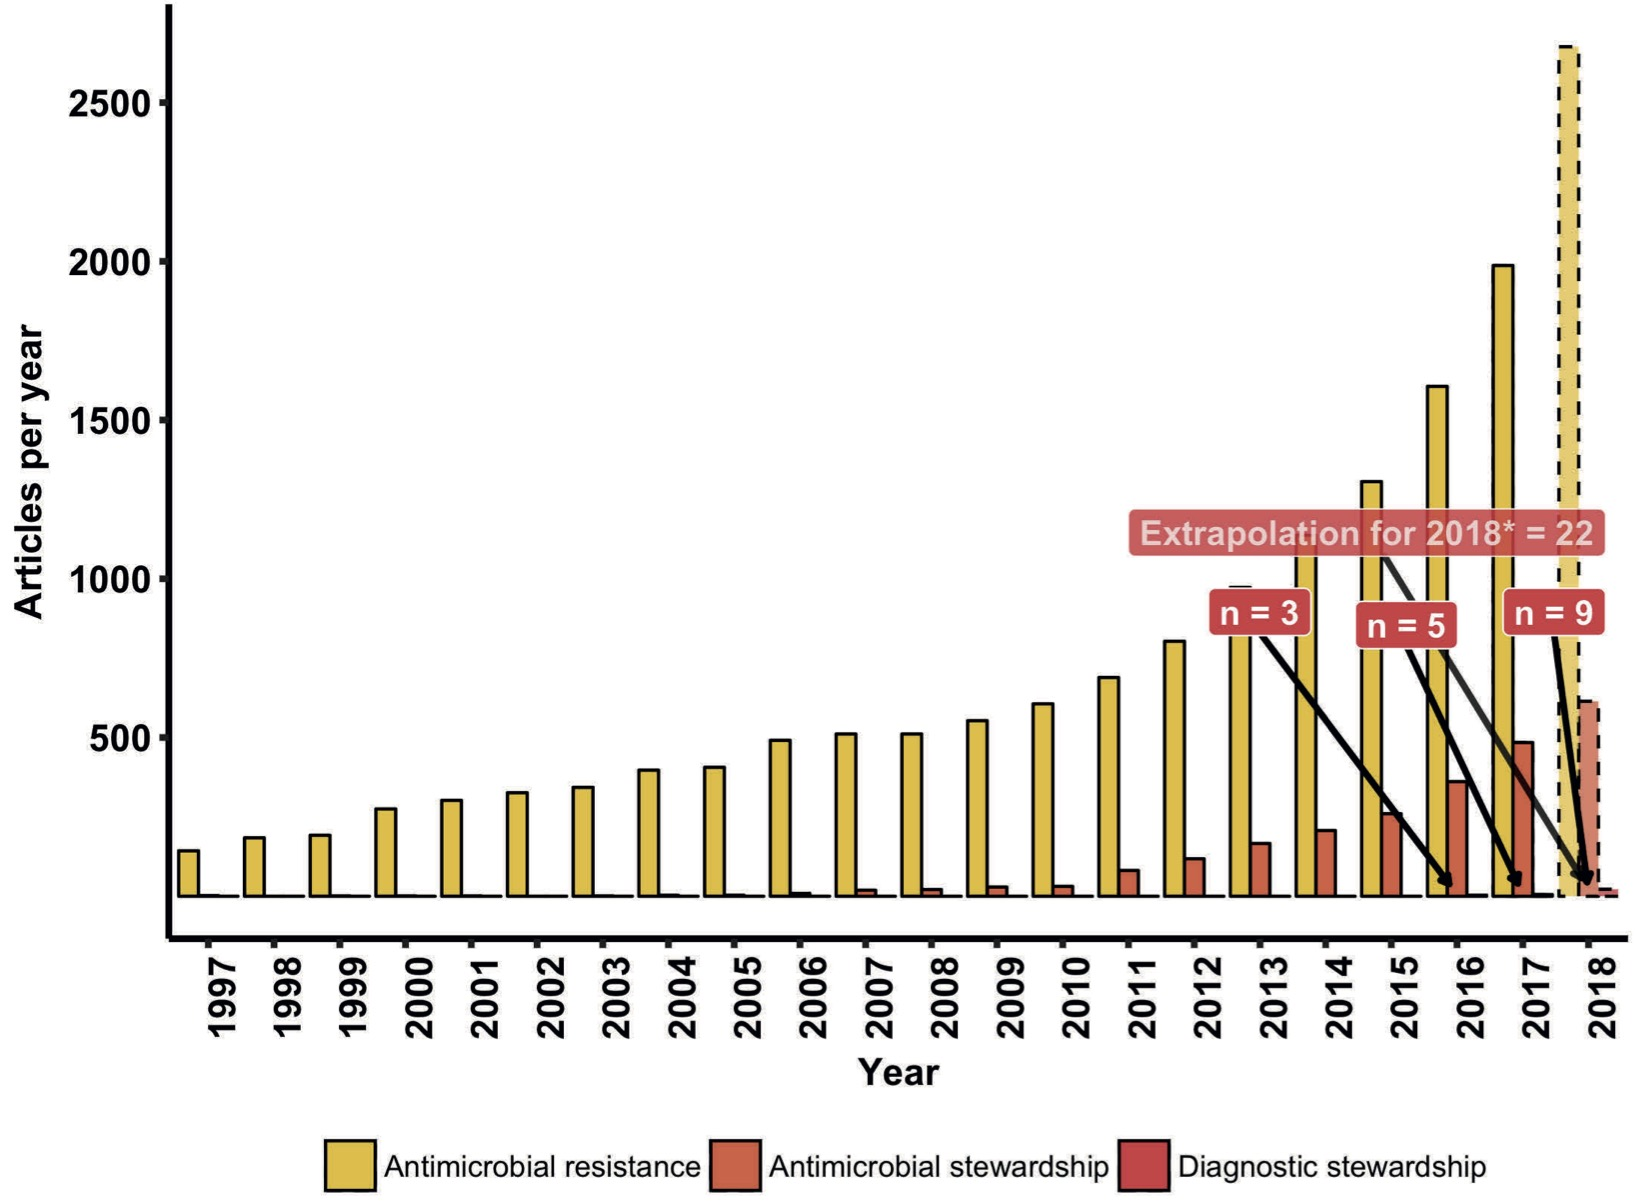
\includegraphics[width=0.8\linewidth]{images/02-01} 

}

\caption{The increase of articles indexed in PubMed. Search strategies: 'antimicrobial stewardship'[Title/Abstract]; 'diagnostic stewardship'[Title/Abstract]; 'antimicrobial resistance'[Title/Abstract]. Source: https://www.ncbi.nlm.nih.gov/pubmed/ (assessed: 2018-05-31). * Extrapolation based on count from 2018-01-01 to 2018-05-31.}\label{fig:fig2-1}
\end{figure}

Nevertheless, the concept of DSP is neither intended to replace other stewardship concepts (in particular ASP) nor to be an alternative. DSP concerns decision making and goes beyond microbiological diagnostics alone. Kahneman \emph{et al.} \textsuperscript{{[}2{]}} said about decision making:

\begin{quote}
We think, each of us, that we're much more rational than we are. And we think that we make our decisions because we have good reasons to make them. Even when it's the other way around. We believe in the reasons, because we've already made the decision. \textsuperscript{{[}2{]}}
\end{quote}

Adequate diagnostics should help us to prevent this kind of situation in medicine by providing a basis to make well-informed decisions. Defining a proper diagnosis is a complex process with several aspects. We believe that DSP is a concept that requires collaboration between different medical specialties for optimal infection management and quality of care. This can include reduced morbidity and/or mortality, unnecessary interventions or treatments, complications, and length of stay. We want to point out why and how DSP affects the entire diagnostic process and that it involves more than just results or turnaround times of microbiological tests. By comparing different patient cases, we want to demonstrate how DSP serves the most important purpose: improved patient care. This involves process optimisation as a basis as well as medical questions and decisions on the individual patient level.

This entire diagnostic process requires multiple decisions along the way of patient care. Guidance and communication on this path are essential because:

\begin{quote}
Intuitive diagnosis is reliable when people have a lot of relevant feedback. But people are very often willing to make intuitive diagnoses even when they're very likely to be wrong. \textsuperscript{{[}3{]}}
\end{quote}

Modern medicine is centred around evidence-based actions and tries to minimise the chance of mistakes while trying to keep the balance between the quality of care and the outcome on one hand and preventing collateral damage and costs on the other hand. In infection management stewardship activities can provide support and guidance in diagnosis and therapy. Physicians can be supported at the bedside to choose the right diagnostic test at the right time for the right patient. The same applies to therapeutic choices: the right treatment at the right time for the right patient in order to achieve the most optimal result. Naturally, these approaches to diagnostic and therapeutic support go hand in hand.

We outline two different case studies - fictitious but nevertheless realistic - of a patient with a prosthetic joint infection (PJI) in different scenarios and different outcomes. These examples underline how interdisciplinary stewardship can lead to a successful outcome for the patient and the physician.

\hypertarget{case-1}{%
\subsection{Case 1}\label{case-1}}

A 70-year-old woman was seen by the orthopaedic surgeon because of chronic pain in her hip prosthesis placed 3 years earlier. An X-ray showed signs of loosening of the prosthesis - an indication for revision surgery. C-reactive protein (CRP) was low (6 mg/L). The diagnosis of aseptic loosening was made, and the patient underwent revision surgery. To rule out low-grade infection, antibiotic prophylaxis was administered only after intraoperative tissue biopsies had been taken for culturing and histology. Cutibacterium acnes (formerly Propionibacterium acnes) was isolated from one out of five tissue biopsies (semi-quantitative \textless1+). Histology showed no indication of inflammation. The positive culture was considered contamination by the attending clinical microbiologist and the patient was discharged without further antibiotic therapy. However, during outpatient follow-up, the patient complained about persistent stiffness of her hip. Three years later, the patient presented again with recurrent loosening of the prosthesis and the presence of a fistula around the surgical site. A second revision intervention was necessary. Due to poor bone quality and poor soft tissue, multiple revisions were needed. Multiple intraoperative tissue biopsies revealed Cutibacterium acnes with the same antibiogram as three years earlier together with a methicillin-sensitive Staphylococcus hominis. The patient was given a cement spacer which made her temporarily immobile and was treated with a high dose of flucloxacillin intravenously. She was discharged with clindamycin per os and re-admitted several months later for reimplantation of the definitive prosthesis. After eight months of revalidation the functional result was poor. The patient permanently walks with support of a cane.

Figure \ref{fig:fig2-2} shows the course of the disease of this patient in which the decision moments are shown in circles. The potential stewardship zone shows the moments when a different action could/should have been taken.

\begin{figure}

{\centering 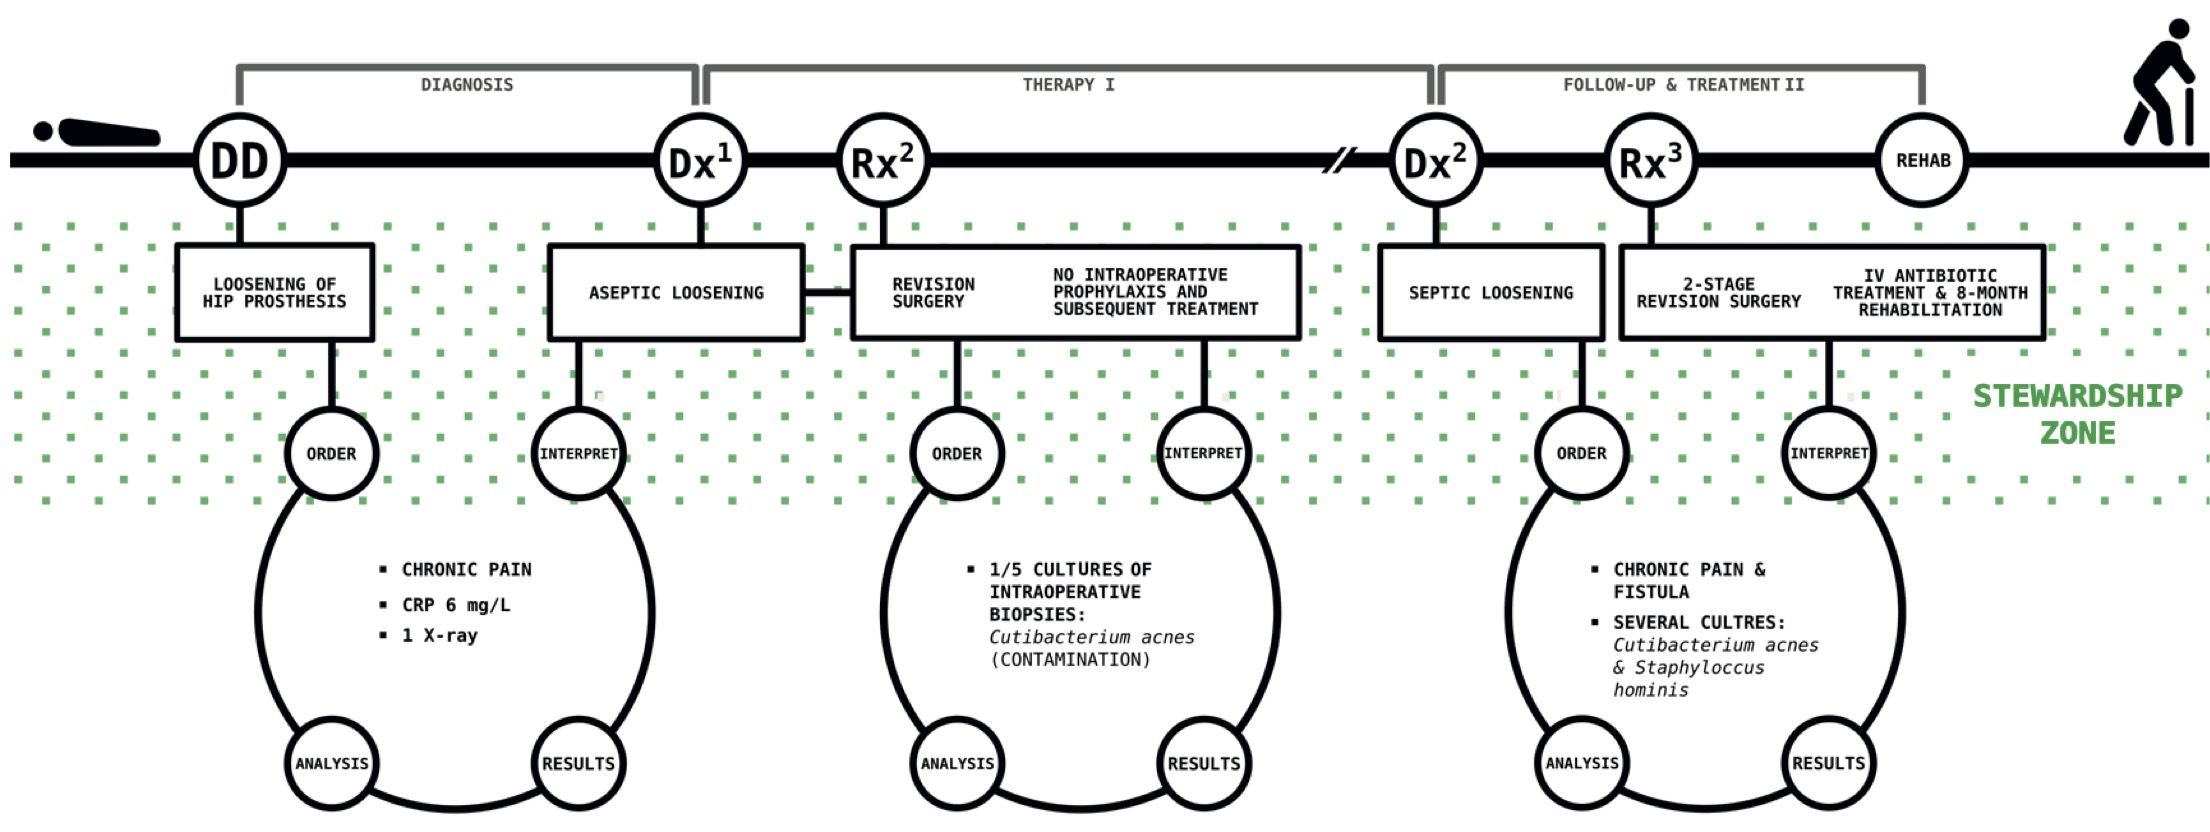
\includegraphics[width=1\linewidth]{images/02-02} 

}

\caption{The first case.}\label{fig:fig2-2}
\end{figure}

The outcome for this patient was certainly not optimal. To illustrate how infection management with stewardship elements can improve the quality of care, a second case of the same patient with a PJI follows. Several additional diagnostic steps were performed (shown in bold) underlining the need for collaboration in stewardship activities including antimicrobial stewardship, of course, and how this affects clinical outcome and hospitalisation.

\hypertarget{case-2}{%
\subsection{Case 2}\label{case-2}}

A 70-year-old woman was seen by the orthopaedic surgeon because of chronic pain in her hip prosthesis placed 3 years earlier. An X-ray showed signs of loosening of the prosthesis - an indication for revision surgery. C-reactive protein (CRP) was low (6 mg/L). The radiologist was consulted to reassess the X-ray taken a year earlier. This image already showed subtle signs of radiolucency around the head and neck of the prosthesis making a mechanical cause of detachment less likely. Synovial fluid was punctured to rule out septic loosening of the prosthesis. The synovial fluid culture remained negative and the leukocyte count was only slightly increased, but several biomarkers were positive suggesting infection (450 mg/L calprotectin and positive alpha-defensin). Subsequently, prior to revision surgery, several tissue biopsies were taken by the orthopaedic surgeon in a sterile environment. Cutibacterium acnes (formerly Propionibacterium acnes) was isolated from one out of five tissue biopsies (5-10 CFU/ml). Histology showed no indication of inflammation. During revision surgery, antibiotic prophylaxis was given prior to surgical incision and several tissue samples were taken for culturing (including sonication) of the prosthesis. Empirical treatment was initiated with high doses of amoxicillin. Due to the previous positive culture with Cutibacterium acnes, all intraoperative cultures were incubated for 14 days on the advice of the clinical microbiologist. C. acnes was found again in two of five tissue biopsies and also in the sonication fluid. These isolates showed the same antibiogram as the isolates from before revision surgery. The patient was then discharged and treated at home with 10 weeks of amoxicillin per os. She fully recovered within a few weeks.

Figure \ref{fig:fig2-3} shows the additional decisions compared to Figure \ref{fig:fig2-2}. These lead to a better outcome for the patient through the implementation of stewardships. The differences with Figure \ref{fig:fig2-2} are shown in red.

\begin{figure}

{\centering 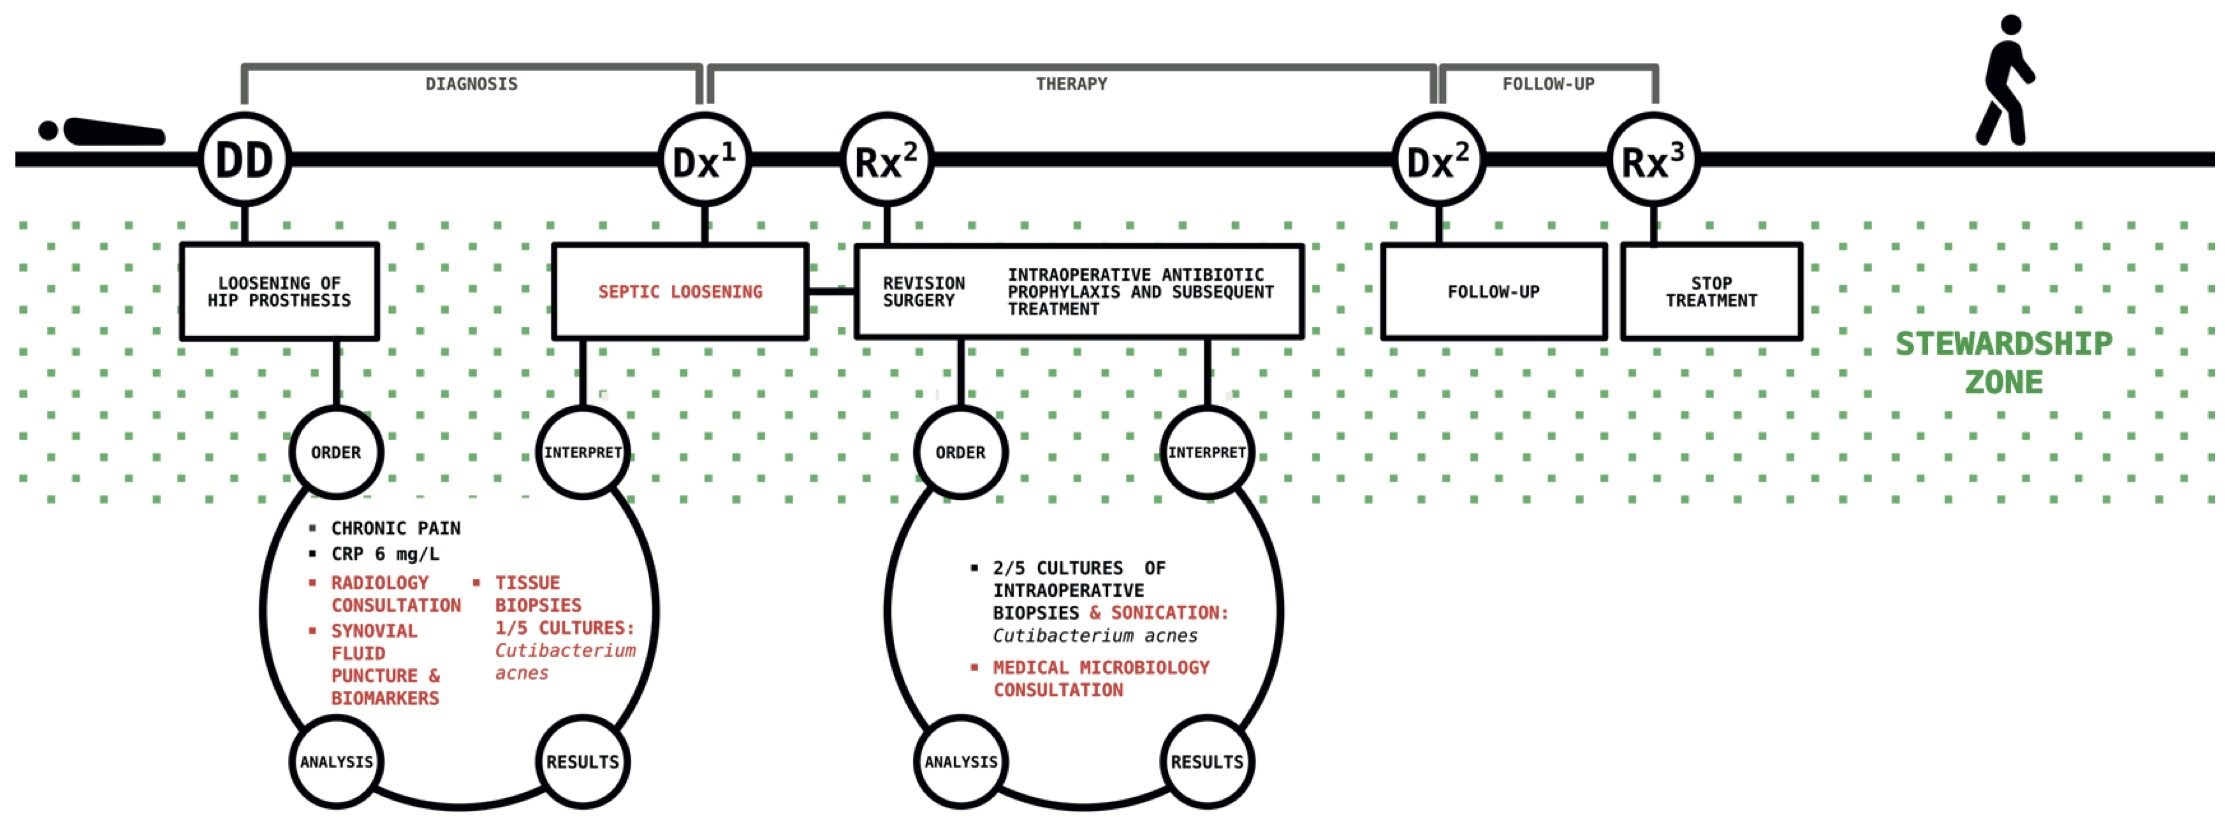
\includegraphics[width=1\linewidth]{images/02-03} 

}

\caption{The second case.}\label{fig:fig2-3}
\end{figure}

\hypertarget{the-general-concept}{%
\section{The general concept}\label{the-general-concept}}

\hypertarget{diagnostics}{%
\subsection{`Diagnostics'}\label{diagnostics}}

The term diagnostics seems simple, but its various aspects are very diverse, as the cases above demonstrate. The second case emphasises the importance of stewardships and centres around facilitating an optimal care process through communication, crossing the boundaries of specialisms, and increasing awareness of the integral nature of successful infection management and optimal quality of care. Different physicians (involved in infection management) and their perceptions are reflected in this view on diagnostics. While some think of the entire process of diagnosing a disease, others think purely of the technical aspect in the lab as diagnostics (of their own speciality). This diversity underlines the importance of communication and collaboration across the boundaries of different medical specialties. The concept of stewardship is widely used to facilitate communication (and clinical decision making). Multiple attempts have been made to establish a clear definition of stewardship, but this has proved challenging \textsuperscript{{[}3,4{]}}. Overall, most of these attempts have been made in the light of antimicrobial stewardship programmes (ASP) and are accompanied by terms such as responsibility, balance, due diligence, and management \textsuperscript{{[}3,4{]}}.

\hypertarget{dsp-in-the-microbiological-laboratory}{%
\subsection{DSP in the microbiological laboratory}\label{dsp-in-the-microbiological-laboratory}}

A medical laboratory usually only has added value if, in addition to the reporting and advice, the range of tests and the test technique meet the requirements of the applicant. The technical aspect of the medical microbiology laboratories has seen tremendous technological advances in recent years. Advanced developments such as sequencing as part the routine to identify isolate properties (e.g., resistance genes) and Matrix-Assisted Laser Desorption/Ionization Time of Flight (MALDI-TOF) mass spectrometry methods have recently revolutionized the laboratories \textsuperscript{{[}5-7{]}}. In addition, many new and fast diagnostic assays such as point-of-care test (POCT) and molecular rapid diagnostic test (mRDT) have entered the market \textsuperscript{{[}8{]}}. The progress is undeniable although integration into workflow, quality control, data storage and availability, added value, and clinical impact often still need to be evaluated.

We embrace these developments but there are two aspects that are really essential for optimal quality of care. Both these aspects can be achieved through stewardship. Firstly, stewardship provides guidance for the appropriate choice of a customised diagnostic strategy for individual patients and patient groups in a specific setting. Guidelines and protocols for diagnostic and appropriate therapeutic choices are key elements in the development of this guidance or steering. A stewardship framework can form the basis for personalised decisions in individual patient care. It has already been demonstrated that new tests such as the aforementioned mRDT are most cost-effective for the diagnosis of bacteraemia when combined with an antimicrobial stewardship programme \textsuperscript{{[}9{]}}. In addition, mRDT is associated with a significant reduction in mortality risk for septic patients but only when combined with ASP \textsuperscript{{[}10{]}}.

Secondly, it is important to consider the entire information loop in a process-oriented way and not just focus on the time-to-result. Stewardship covers this loop and starts making choices at the bedside. In addition, the interpretation of test results and timely feedback are equally important in order to be able to make good, evidence-based, and rapid therapy adjustments when needed. For example, physicians considering starting non-prophylactic intravenous antimicrobial treatment should (almost) always take blood cultures before starting. Although this is standard care and described in international guidelines \textsuperscript{{[}11{]}}, compliance is only 30 to 50\% {[}12, 13, Luz \emph{et al.}; unpublished data{]}. Only through complete `loops', from bedside to bedside, can better technology and improved work processes in microbiology laboratories be extended and made to work to their full potential.

\hypertarget{dsp-as-process-optimisation}{%
\subsection{DSP as process optimisation}\label{dsp-as-process-optimisation}}

Turnaround times (TAT) are a commonly used but poorly defined term in many areas. In a systematic review, a total of 61 different TAT definitions (out of a total of 151) were found to be used in several clinical areas \textsuperscript{{[}14{]}}. Of those, only 10 definitions cover the time from test order placement to the time at which the results are being viewed by the ordering physician (Figure \ref{fig:fig2-4}).

\begin{figure}

{\centering 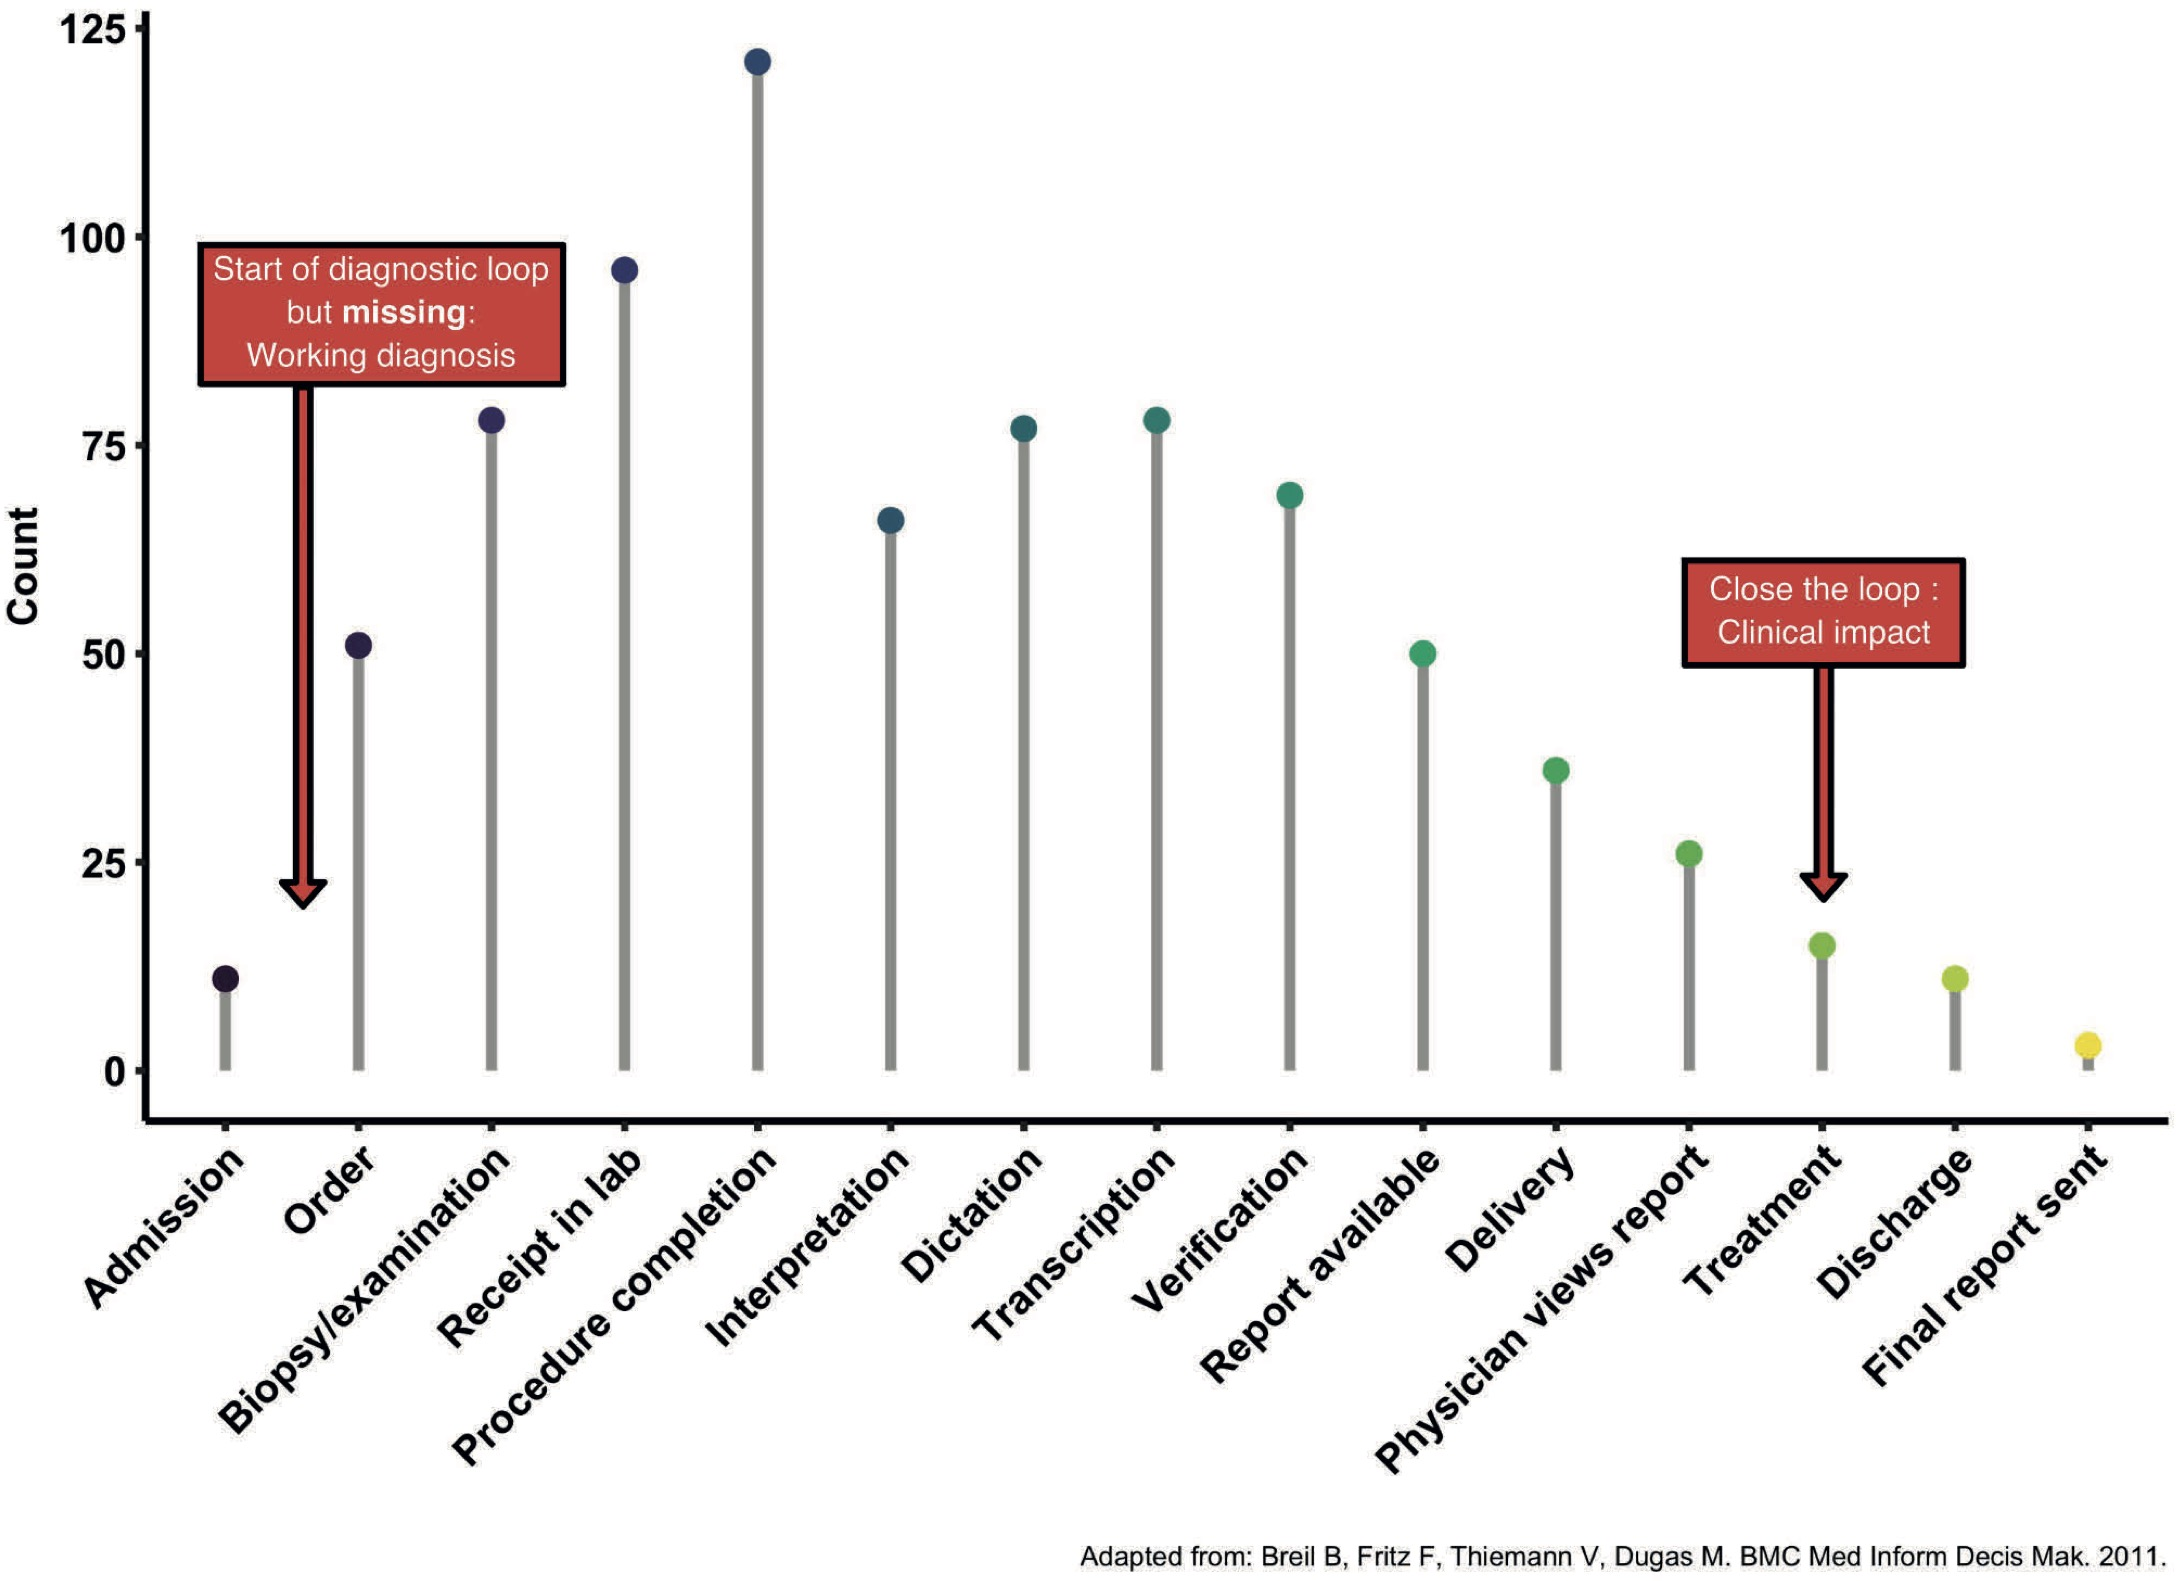
\includegraphics[width=1\linewidth]{images/02-04} 

}

\caption{Time points mentioned in TAT definitions.}\label{fig:fig2-4}
\end{figure}

Nevertheless, even the order of a test is a decision within a diagnostic loop and should be taken into account when time is measured. We are convinced that infection management can help to understand the importance of a full loop from moment of choice to moment of choice, from the bedside to a diagnostic result and back. This implies the time from the moment when the need for diagnostics becomes clear, to the time when it can be acted upon based on its results. We call this time to action which is indicated by a red arrow in Figure \ref{fig:fig2-4}.

\hypertarget{multidisciplinary-aspects-of-dsp-and-infection-management}{%
\subsection{Multidisciplinary aspects of DSP and infection management}\label{multidisciplinary-aspects-of-dsp-and-infection-management}}

It is essential to realise that the information needed to assess this time to action does not come only from microbiological laboratories. Communication and collaboration in the stewardship zone (Figures 2 and 3) are key and this applies to all specialities. But what would be the effect on the patient if microbiological diagnostics were not led by DSP when there is already good communication and cooperation in place? Would DSP no longer be necessary? Or is good cooperation equivalent to DSP?

DSP can significantly reduce the time to action by making proper use of each other's expertise to make optimal decisions for the patient. In practice, information from one diagnostic discipline can help to steer the diagnostic process of another diagnostic discipline. One reason for this is that during the diagnostic process of many disciplines, such as medical microbiology and imaging, an intrinsic amount of interpretation takes place. The clinical course is no less important here. We always need DSP, because together we try to act as optimally as possible in the interest of the patient, in which diagnosis is an important tool. DSP is not specific to medical microbiology, as demonstrated by the relevance of its collaboration with radiology in case 2. Nor is it specific to any other speciality. DSP is not intended as a reactive ad hoc solution but rather as a proactive, structural approach. DSP should be seen as guiding the entire diagnostic process, not only on the basis of antibiotics, but also on the basis of extensive imaging (such as for endocarditis), biomarkers (such as leukocytes and CRP, or procalcitonin for de-escalation of treatment), or by therapeutic drug monitoring (TDM) modelling the optimal dosage from the start of (empirical) treatment for individual patients and patient groups. One form of diagnostics is relevant to monitor trends, the other to directly answer a clinical question. This does not mean that one is less important than the other or that we should look at the value of an antibiogram differently from the value of a therapeutic drug monitoring. A pharmacist is also part of DSP.

As an example, in Dutch hospitals we are used to having a hospital pharmacist in house, providing clinical pharmaceutical services. Consultations are typically performed via e-mail, telephone, or an electronic prescription system. On the other hand, in countries such as the United Kingdom, these pharmacists work in infection management in the clinical (nursing) departments on a daily basis in collaboration with other specialists. This supports the most safe, appropriate, and cost-effective antimicrobial treatment \textsuperscript{{[}15{]}}. In addition, as mentioned earlier, the guidance of antimicrobial therapy by TDM is another important aspect. Hospital pharmacists can make suggestions on sample timing for TDM, inform about early prediction of attainable levels and dose adjustments to achieve adequate exposure and reduce toxicity as quickly as possible, and interpret results \textsuperscript{{[}16{]}}. As a result, they are an integral part of the stewardship concept. We are convinced that the different stewardship terms and concepts form synergy for the best infection management \textsuperscript{{[}1,17{]}}. Infection management has different aspects (such as ASP) and stewardship refers to guidance provided by focused experts \textsuperscript{{[}18{]}}.

Empirical antimicrobial therapy is a good example to illustrate how these aspects are linked. The working diagnosis (see also cases 1 and 2), based on an appropriate differential diagnosis, forms the basis for an appropriate empirical therapy that takes into account the most relevant pathogens, their anticipated susceptibility, the source of infection (taking into account the compartment), and underlying patient factors. Adequate initial diagnostic initiatives (such as deep focus puncture, see case 2) may simultaneously be therapeutic (such as surgical/interventional drainage for source control). Vice versa, the clinical course under therapy can be diagnostic in itself, for example, if diagnostics for the working diagnosis are correct and complete. Ultimately, the treatment of patients with complex infections almost always requires targeted treatment. This, in turn, requires adequate initial and ongoing diagnostics for optimal treatment. Figure \ref{fig:fig2-5} shows the decision moments and different specialisms that can be involved in this whole process.

\begin{figure}

{\centering 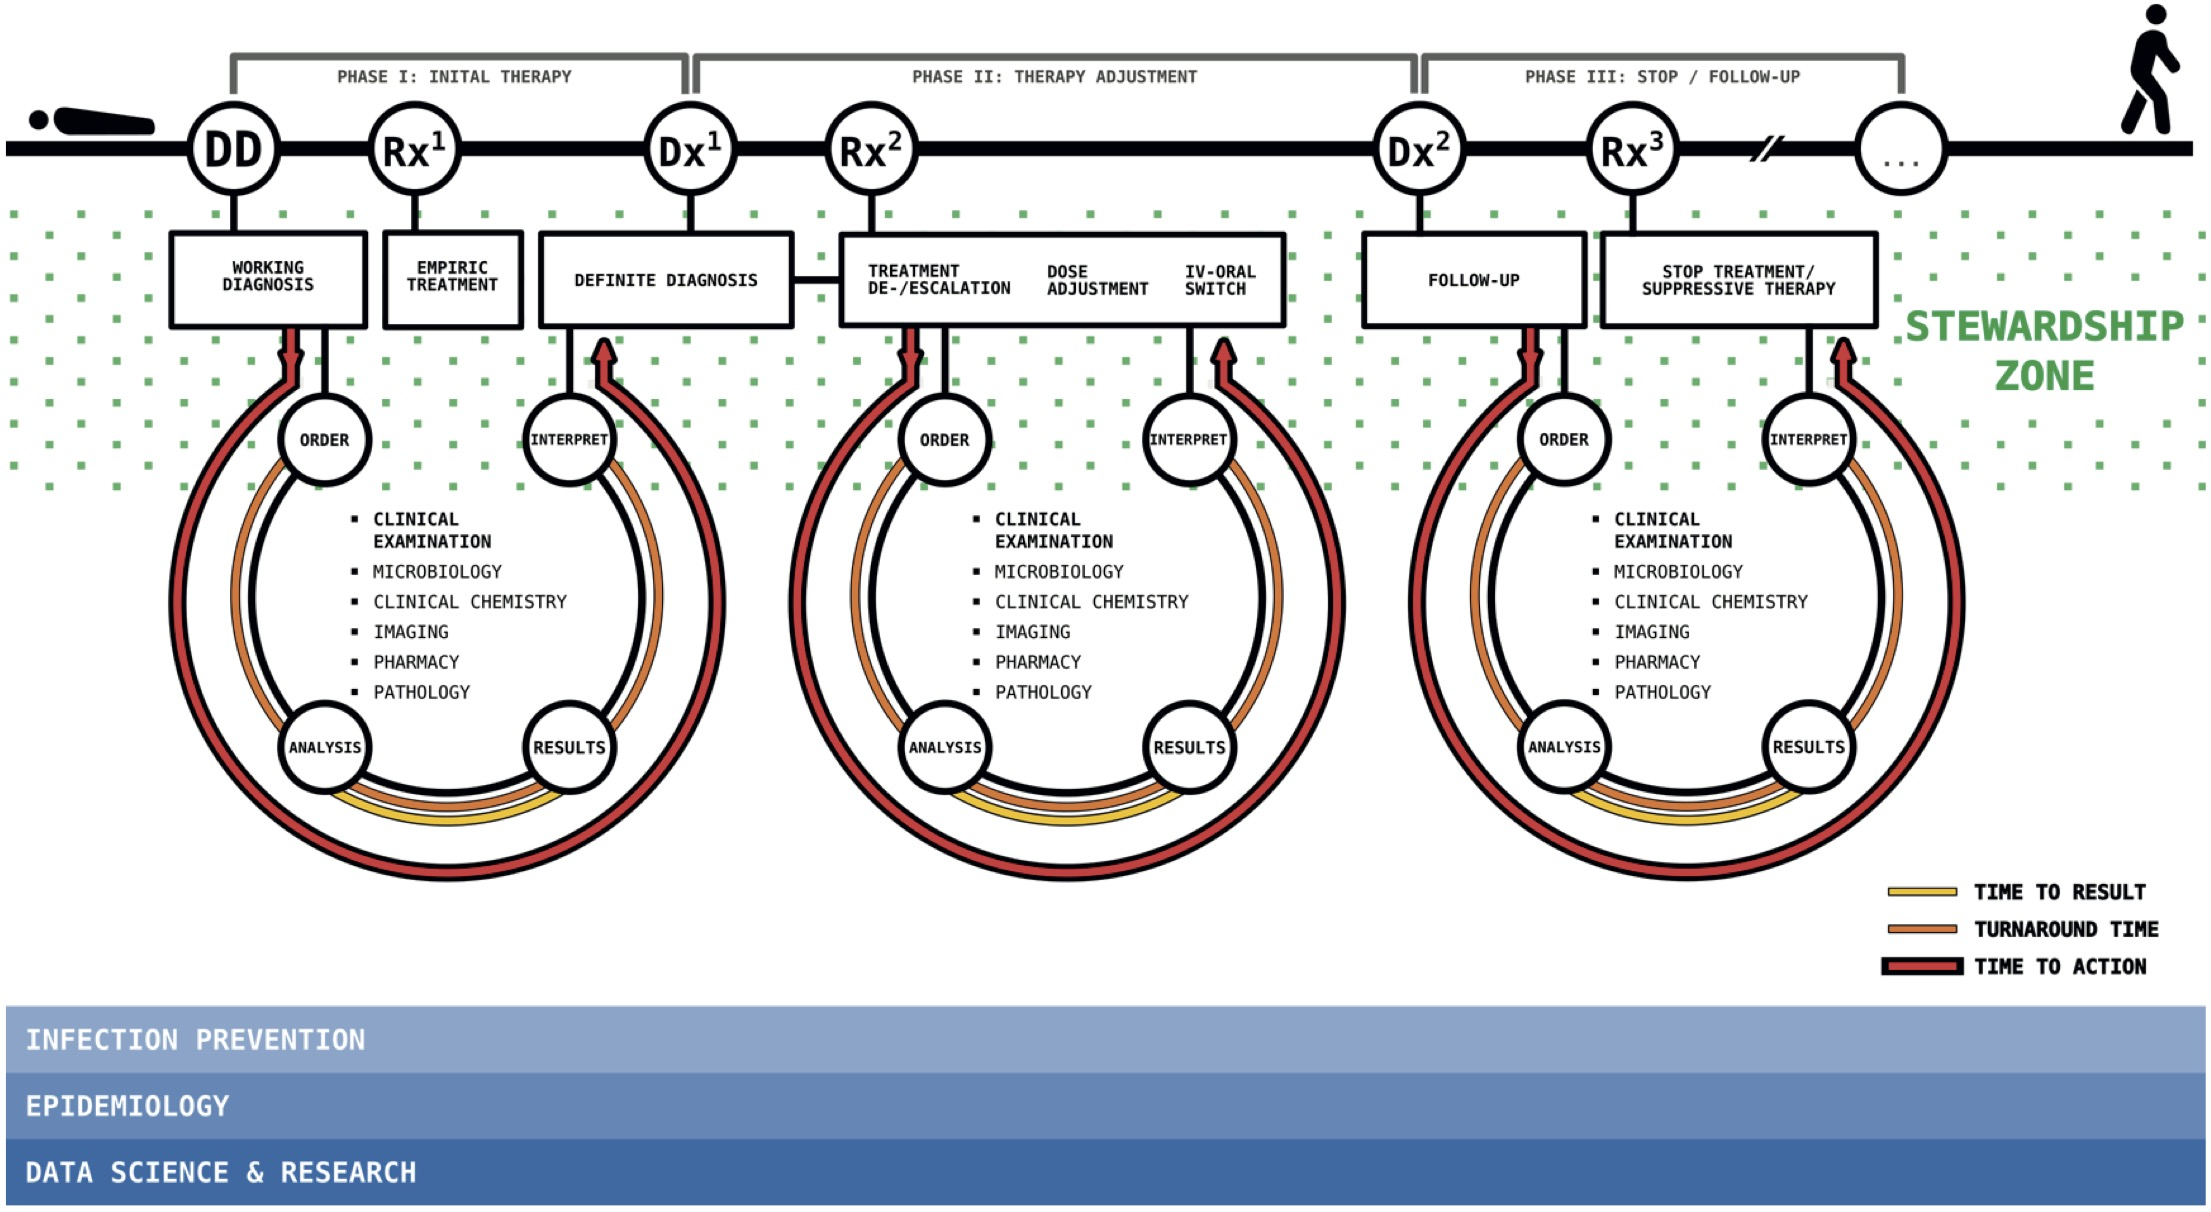
\includegraphics[width=1\linewidth]{images/02-05} 

}

\caption{Stewardship in infection management.}\label{fig:fig2-5}
\end{figure}

\hypertarget{conclusion}{%
\section{Conclusion}\label{conclusion}}

The answer to the question from the title (Diagnostic stewardship - sentence or nonsense?!) is: both. It is nonsense to debate terminology and the discussion about differences between diagnostic stewardship and infection management is only of semantic nature. Diagnostic stewardship makes sense in the concept discussed above. It can guide specialists (physician-microbiologist/medical-molecular microbiologists and experts from other fields, such as hospital pharmacists, radiologists, nuclear medicine, etc.) to the area of the stewardship zone of interaction and communication (Fig. 5), where they can bring in their expertise to complex clinical decision-making. Clinical information, including a patient's clinical development, is extremely important for correctly interpreting diagnostic results and steering the process. It can also help leading clinicians and other clinicians to understand the full potential (and limitations) of diagnostics and how important they are for evidence-based decision-making. We follow an integrated stewardship model that adds different perspectives (antimicrobial, infection prevention, and diagnostic stewardship - AID) to the ultimate goal of all stewardship intentions - the best quality care for the individual patient \textsuperscript{{[}1{]}}.

Stewardship consists largely of translation and communication during the decision-making process. Diagnostics are essential in this. But there is no need for a new name. Diagnostic stewardship as a name may be without added value and more and more use of stewardship-like terms could lead to confusion. The aim of all efforts and experts in infection management is the same: to improve quality of care and patient outcomes. We see with our own eyes how DSP guidelines are adhered to and realise how important it is that we continue to emphasise the often-underexposed diagnostic aspects of infection management. Multidisciplinary management based on diagnostics builds the basis for optimal outcomes for patients with infections.

\hypertarget{financing}{%
\section*{Financing}\label{financing}}
\addcontentsline{toc}{section}{Financing}

This study was partly supported by the INTERREG V A (202085) funded project EurHealth-1Health (\url{http://www.eurhealth1health.eu}), part of a Dutch-German cross-border network supported by the European Commission, the Dutch Ministry of Health, Welfare and Sport, the Ministry of Economy, Innovation, Digitalisation and Energy of the German Federal State of North Rhine-Westphalia and the Ministry for National and European Affairs and Regional Development of Lower Saxony.

In addition, this study was part of a project funded by the European Union's Horizon 2020 research and innovation programme under the Marie Sklodowska-Curie grant agreement 713660 (MSCA-COFUND-2015-DP ``Pronkjewail'').

\hypertarget{references-1}{%
\section*{References}\label{references-1}}
\addcontentsline{toc}{section}{References}

\begin{enumerate}
\def\labelenumi{\arabic{enumi}.}
\tightlist
\item
  Dik J-WH, Poelman R, Friedrich AW, Panday PN, Lo-Ten-Foe JR, van Assen S, \emph{et al.} An integrated stewardship model: antimicrobial, infection prevention and diagnostic (AID). Future Microbiol. 2016;11(1):93--102.
\item
  Kahneman D. Thinking, fast and slow. Macmillan; 2011.
\item
  Dyar OJ, Huttner B, Schouten J, Pulcini C, ESGAP (ESCMID Study Group for Antimicrobial stewardshiP). What is antimicrobial stewardship? Clin Microbiol Infect. 2017 Nov;23(11):793--8.
\item
  Mendelson M, Balasegaram M, Jinks T, Pulcini C, Sharland M. Antibiotic resistance has a language problem. Nature. 2017 May 3;545(7652):23--5.
\item
  Greub G, Moran-Gilad J, Rossen J, Egli A, ESCMID Study Group for Genomic and Molecular Diagnostics (ESGMD). ESCMID postgraduate education course: applications of MALDI-TOF mass spectrometry in clinical microbiology. Microbes Infect. 2017 Sep;19(9-10):433--42.
\item
  Didelot X, Bowden R, Wilson DJ, Peto TEA, Crook DW. Transforming clinical microbiology with bacterial genome sequencing. Nat Rev Genet. 2012 Sep;13(9):601--12.
\item
  Greninger AL. The challenge of diagnostic metagenomics. Expert Rev Mol Diagn. 2018 Jun 18;1--11.
\item
  Kozel TR, Burnham-Marusich AR. Point-of-Care Testing for Infectious Diseases: Past, Present, and Future. J Clin Microbiol. 2017 Aug;55(8):2313--20.
\item
  Pliakos EE, Andreatos N, Shehadeh F, Ziakas PD, Mylonakis E. The Cost-Effectiveness of Rapid Diagnostic Testing for the Diagnosis of Bloodstream Infections with or without Antimicrobial Stewardship. Clin Microbiol Rev.~2018 Jul;31(3).
\item
  Timbrook TT, Morton JB, McConeghy KW, Caffrey AR, Mylonakis E, LaPlante KL. The Effect of Molecular Rapid Diagnostic Testing on Clinical Outcomes in Bloodstream Infections: A Systematic Review and Meta-analysis. Clin Infect Dis. 2017 Jan 1;64(1):15--23.
\item
  Rhodes A, Evans LE, Alhazzani W, Levy MM, Antonelli M, Ferrer R, \emph{et al.} Surviving Sepsis Campaign: International Guidelines for Management of Sepsis and Septic Shock: 2016. Crit Care Med. 2017 Mar;45(3):486--552.
\item
  Reissig A, Mempel C, Schumacher U, Copetti R, Gross F, Aliberti S. Microbiological diagnosis and antibiotic therapy in patients with community-acquired pneumonia and acute COPD exacerbation in daily clinical practice: comparison to current guidelines. Lung. 2013 Jun;191(3):239--46.
\item
  Shallcross LJ, Freemantle N, Nisar S, Ray D. A cross-sectional study of blood cultures and antibiotic use in patients admitted from the Emergency Department: missed opportunities for antimicrobial stewardship. BMC Infect Dis. 2016 Apr 18;16:166.
\item
  Breil B, Fritz F, Thiemann V, Dugas M. Mapping turnaround times (TAT) to a generic timeline: a systematic review of TAT definitions in clinical domains. BMC Med Inform Decis Mak. 2011 May 24;11:34.
\item
  Wickens HJ, Jacklin A. Impact of the Hospital Pharmacy Initiative for promoting prudent use of antibiotics in hospitals in England. J Antimicrob Chemother. 2006 Dec;58(6):1230--7.
\item
  van Wanrooy MJP, Rodgers MGG, Span LFR, Zijlstra JG, Uges DRA, Kosterink JGW, \emph{et al.} Voriconazole Therapeutic Drug Monitoring Practices in Intensive Care. Ther Drug Monit. 2016 Jun;38(3):313--8.
\item
  Pulcini C, Binda F, Lamkang AS, Trett A, Charani E, Goff DA, \emph{et al.} Developing core elements and checklist items for global hospital antimicrobial stewardship programmes: a consensus approach. Clin Microbiol Infect \textsuperscript{{[}Internet{]}}. 2018 Apr 3; Available from: \url{http://dx.doi.org/10.1016/j.cmi.2018.03.033}
\item
  British Society for Antimicrobial Chemotherapy. Antimicrobial Stewardship: From Principal to Practice \textsuperscript{{[}Internet{]}}. Birmingham, United Kingdom: British Society for Antimicrobial Chemotherapy; 2018. Available from: \url{http://bsac.org.uk/antimicrobial-stewardship-from-principles-to-practice-e-book/}
\end{enumerate}

\hypertarget{ch03-introducing-new-method}{%
\chapter{Introducing a New, Free, and Independent Method for Standardised, Reproducible and Reliable Analyses of Antimicrobial Resistance Data}\label{ch03-introducing-new-method}}

In preparation

(as of date of PhD defence: 25 August 2021)

Berends MS \textsuperscript{1,2}, Luz CF \textsuperscript{2}, Sinha BNM \textsuperscript{2}, Glasner C \textsuperscript{2‡}, Friedrich AW \textsuperscript{2‡}

\begin{enumerate}
\def\labelenumi{\arabic{enumi}.}
\tightlist
\item
  Certe Medical Diagnostics \& Advice Foundation, Groningen, the Netherlands
\item
  University of Groningen, University Medical Center Groningen, Department of Medical Microbiology \& Infection Control, Groningen, the Netherlands
\end{enumerate}

\textsuperscript{‡} These authors contributed equally

\hypertarget{abstract-1}{%
\section*{Abstract}\label{abstract-1}}
\addcontentsline{toc}{section}{Abstract}

As the burden of antimicrobial resistance (AMR) is continuously increasing, reliable and reproducible data and data analysis are of utmost importance. Conducting AMR data analysis is challenging since it requires (1) a thorough understanding of (clinical) epidemiology; (2) expertise in (clinical) microbiology and infectious diseases; (3) experience in microbiological data analysis; (4) availability of reference data, such as the biological taxonomy of microorganisms and defined daily doses (DDD) for antimicrobials; and (5) availability of (inter-)national guidelines and software methods to apply them. Furthermore, data stored in laboratory information systems lack the right structure, (inter-) national guidelines for interpreting raw laboratory test results cannot be easily applied, and scientifically reliable reference data about microorganisms and antimicrobial agents are not readily available. To fill this gap, we developed a free, independent, and open-source software solution to cover all those aspects of working with AMR data. The AMR package for R enables AMR data analysis for research and clinical workflows alike. Through an online survey package users reported more reproducibility of analysis results (83\%), more reliable outcomes of AMR analyses (72\%), and new or improved insight into AMR patterns (61\%). The AMR package was also used to support clinical decision-making (44\%) and for clinical research (28\%). Our first insights into the usage and the usability of the AMR package confirm that this package is fulfilling its intended aim, as regional, national, and international organisations already use the package to support clinical decision-making in infection management. The flexible open-source design also enables rapid integration of updated guidelines (e.g., new EUCAST breakpoints) and setting-specific adaptations are encouraged. Together, the AMR package for R can thus empower any specialist in the field working with AMR data by providing a comprehensive toolbox of solutions for AMR data analyses.

\hypertarget{background}{%
\section{Background}\label{background}}

As the burden of antimicrobial resistance (AMR) is continuously increasing, surveillance programs with reliable and reproducible data and data analysis methods are of utmost importance for controlling and streamlining efforts to curb AMR \textsuperscript{{[}1,2{]}}. To guide these efforts and to support clinical decision-making and infection-control interventions, AMR data analysis has to be conducted in a clinically and epidemiologically sensible way \textsuperscript{{[}3{]}}. Conducting AMR data analysis is challenging since it requires (1) a thorough understanding of (clinical) epidemiology; (2) expertise in (clinical) microbiology and infectious diseases; (3) experience in microbiological data analysis; (4) availability of reference data, such as the biological taxonomy of microorganisms and defined daily doses (DDD) for antimicrobials; and (5) availability of (inter-)national guidelines and software methods to apply them.

Moreover, AMR data analysis is often also hindered by three key aspects. Firstly, data stored in microbiological laboratory information systems (LIS) are typically not readily suitable for (epidemiological) data analyses. LIS were initially designed to fit result registration and billing purposes rather than AMR data analysis. Consequently, fundamental requirements for (epidemiological) data analyses are often lacking, such as isolate selection criteria, phenotypic determination of (multi-)drug resistance, and the ability to extract data for analysis in an automated, structured, fast, and reliable way. Moreover, data analyses that require data from multiple LIS sources (e.g., in multi-centre studies) face major barriers in data aggregation which, to the best of our knowledge, cannot be solved by currently available commercial software solutions. Besides, as applications of artificial intelligence are expected of being increasingly developed in the coming years, also in clinical microbiology, microbiological data technologies and structures need to become compatible for these future applications.

Secondly, AMR data analysis depends on (inter-)national standards and guidelines for the interpretation of raw laboratory measurements and the reporting of AMR results. In Europe, guidelines from the European Committee on Antimicrobial Susceptibility Testing (EUCAST) are the predominantly implemented set of rules in clinical microbiological laboratories \textsuperscript{{[}4,5{]}}. LIS need to be well-maintained to be able to integrate continuous guideline updates. In our experience, this maintenance can often not be guaranteed and depends on the availability of local or external software support services. This is further hindered by the current distribution of manually formatted guidelines in Microsoft Excel and Portable Document Format (PDF) formats that are not often readily machine-readable. LIS maintainers, in collaboration with clinical staff, are therefore forced to manually implement updated guidelines which can be time-consuming and error-prone

Thirdly, reliable AMR data analysis depends on taxonomic reference data to interpret raw LIS data using AMR interpretation guidelines, such as EUCAST Expert Rules and EUCAST Clinical Breakpoints \textsuperscript{{[}5,6{]}}. Unfortunately, typical LIS contain local, static taxonomic data. We found that these data are often poorly maintained. We collected the taxonomic names of bacteria used in clinical reports from seven different public health institutions in the Netherlands which cover microbiological diagnostics in hospitals and primary care for 15\% of the total Dutch population. The taxonomic names were compared to publicly available and authoritative reference databases; the Catalogue of Life and the List of Prokaryotic names with Standing in Nomenclature (LPSN, previously known as the Deutsche Sammlung von Mikroorganismen und Zellkulturen, DSMZ) \textsuperscript{{[}7,8{]}}. We found that all participating institutions reported taxonomic names in clinical reports that did not match current taxonomic standards according to reference databases. For example, \emph{Enterobacter aerogenes} and \emph{Enterobacter massiliensis} were renamed \emph{Klebsiella aerogenes} and \emph{Metakosakonia massiliensis} respectively in 2017 \textsuperscript{{[}9,10{]}}. LIS that are not kept up to date are consequently not entirely compatible with recent interpretation guidelines. Given that AMR guidelines are strongly based on the microbial taxonomy (some rules only apply to a specific genus, other rules apply to a specific family) it is crucial that this information is correct and kept up to date. In the studied institutions, the lag between the reported taxonomic names and the taxonomic standard was up to 41 years as of March 2021.

\hypertarget{standardising-amr-data-analysis}{%
\section{Standardising AMR data analysis}\label{standardising-amr-data-analysis}}

Previously, no dedicated software solution was available to address all aforementioned aspects. To fill this gap, we developed a free, independent, and open-source software solution to cover all those aspects of working with AMR data. The AMR package for R \textsuperscript{{[}11{]}} provides functionalities that enable standardised and reproducible workflows from any raw LIS data to results ready to publish, for research and clinical workflows alike. The AMR package for R was developed with a team of contributors from 12 public health organisations in seven countries aiming to be used in any research or clinical setting where (epidemiological) data analysis of microorganisms, AMR, or antimicrobial agents is required. It is independent of any other software solution and was designed to work in any setting, including those with limited computational and financial resources.

With this AMR package, we aimed at providing: (1) tools to simplify AMR data cleaning, transformation, and analysis; (2) methods to easily incorporate (inter)national guidelines; and (3) scientifically reliable reference data, including the aforementioned aspects. The AMR package enables standardised and reproducible AMR data analysis with the application of evidence-based rules (e.g., EUCAST expert rules for intrinsic resistance), the selection of first isolates, the translation of various codes for microorganisms and antimicrobial agents, determination of (multi-)drug-resistant microorganisms, and the calculation of antimicrobial resistance rates, prevalence, and future trends. The AMR package supports all EUCAST MIC/disk diffusion interpretation guidelines from 2011 until 2021 and EUCAST Expert rules versions 3.1 (2016) and 3.2 (2020) \textsuperscript{{[}12,13{]}} In addition, the AMR package supports all CLSI MIC/disk diffusion interpretation guidelines from 2011 until 2019 (non-veterinary only). For all mentioned guidelines, files readable for LIS are provided for easy implementation.

As of 30 April 2021, the AMR package for R has been downloaded from 162 countries since its first release in early 2018 (Figure \ref{fig:fig3-1}), according to data from a popular public repository where users can download R packages. After 19 releases, the median number of downloads per release is 2,548 (range: 269-5,050).

\begin{figure}

{\centering 
\includegraphics[width=1\linewidth]{images/03-01} 

}

\caption{Countries (grey, n = 162) with registered downloads of the AMR package for R between March 2018 and April 2021. Sources: cran.rstudio.org and cloud.r-project.org.}\label{fig:fig3-1}
\end{figure}

A technical validation of the AMR package has been accepted for publication \textsuperscript{{[}11{]}}. Additionally, it has been clinically and epidemiologically validated in a tertiary care hospital and across seven clinical microbiology laboratories in the Netherlands {[}Berends \emph{et al.}, unpublished, see chapter 6 and 7 of this thesis{]}. Moreover, the AMR package has already been used in several scientific publications that focused on different aspects in the field of AMR \textsuperscript{{[}14--17{]}}.

\hypertarget{comparison-with-existing-software-methods}{%
\section{Comparison with existing software methods}\label{comparison-with-existing-software-methods}}

Popular statistical software such as SPSS, Stata and SAS, focus on a broad implementation of statistical functions but are proprietary software, disallowing users to freely use, modify, or share the software. This also prohibits extending the software by unaffiliated developers. Since R is free, open software and extendible, users and developers can contribute to the software, to which end the AMR package is a practical example.

Other free software alternatives for AMR data analysis exist, for example WHONET, a free microbiology laboratory database software supported by the WHO \textsuperscript{{[}18{]}}. WHONET allows manual data entry from LIS reports and provides AMR interpretation using recent CLSI and EUCAST guidelines with a particular focus on AMR surveillance. Results from WHONET can also be shared to surveillance programs such as the European Antimicrobial Resistance Surveillance Network (EARS-Net) and the WHO Global Antimicrobial Resistance Surveillance System (GLASS). Yet, the latest release, WHONET 2020, does not provide tools for cleaning and transforming data and relies on outdated EUCAST guidelines. Furthermore, we found a lag between the included taxonomic database and the current taxonomic standard of up to 59 years (median 7 years). Another alternative of a free software program is Epi Info which is provided by the United States Centers for Disease Control and Prevention (CDC) and aims at public health practitioners and researchers \textsuperscript{{[}19{]}}. While Epi Info provides statistical and epidemiological methods for analysing data, it does not offer tools nor reference data for working with AMR test results or antimicrobial drugs, thus, ruling out the option for dedicated AMR data analysis. With the AMR package for R, an open and dedicated software solution is available that covers all aspects of working with AMR data.

\hypertarget{user-feedback}{%
\section{User feedback}\label{user-feedback}}

In July 2020, we published a survey on the website created for this package (\url{https://msberends.github.io/AMR}) to seek voluntary feedback from package users about user backgrounds and usage of the AMR package. Until December 2020, 18 participants completed the survey. Participants have used the AMR package in Australia, Colombia, Egypt, France, Germany, Haiti, India, Mali, Mexico, the Netherlands, Nigeria, Philippines, Spain, Sweden, and the United Kingdom.

Participants were asked to rate their experience in the statistical programming language R and in using the AMR package on a scale from 1 (not experienced/useful) to 10 (very experienced/useful). The overall experience in R was reported with a median of 7 (range: 4-9)., whereas Ssuit ability for AMR analyses using the AMR package was rated with a median of 9 (range: 6-9). The participants rated the usefulness of the AMR package for their work with a median of 9 (range: 5-9). The convenience of the included software functions was rated with a median of 8 (range: 6-9) and the documentation of the AMR package was rated with a median of 8.5 (range: 7-10). Of all participants, 83\% reported more reproducibility of analysis results and, 72\% reported more reliable outcomes of AMR analyses (Figure \ref{fig:fig3-2}). Notably, 61\% reported new or improved insight into AMR for their institution or region. The AMR package was also used to support clinical decision-making (44\%) and for clinical research (28\%). Furthermore, 66\% reported a faster and streamlined analysis workflow and 39\% reported improved communicating analysis results. In 33\%, participants started using R more often because of the capabilities that the AMR package provides.

\begin{figure}

{\centering 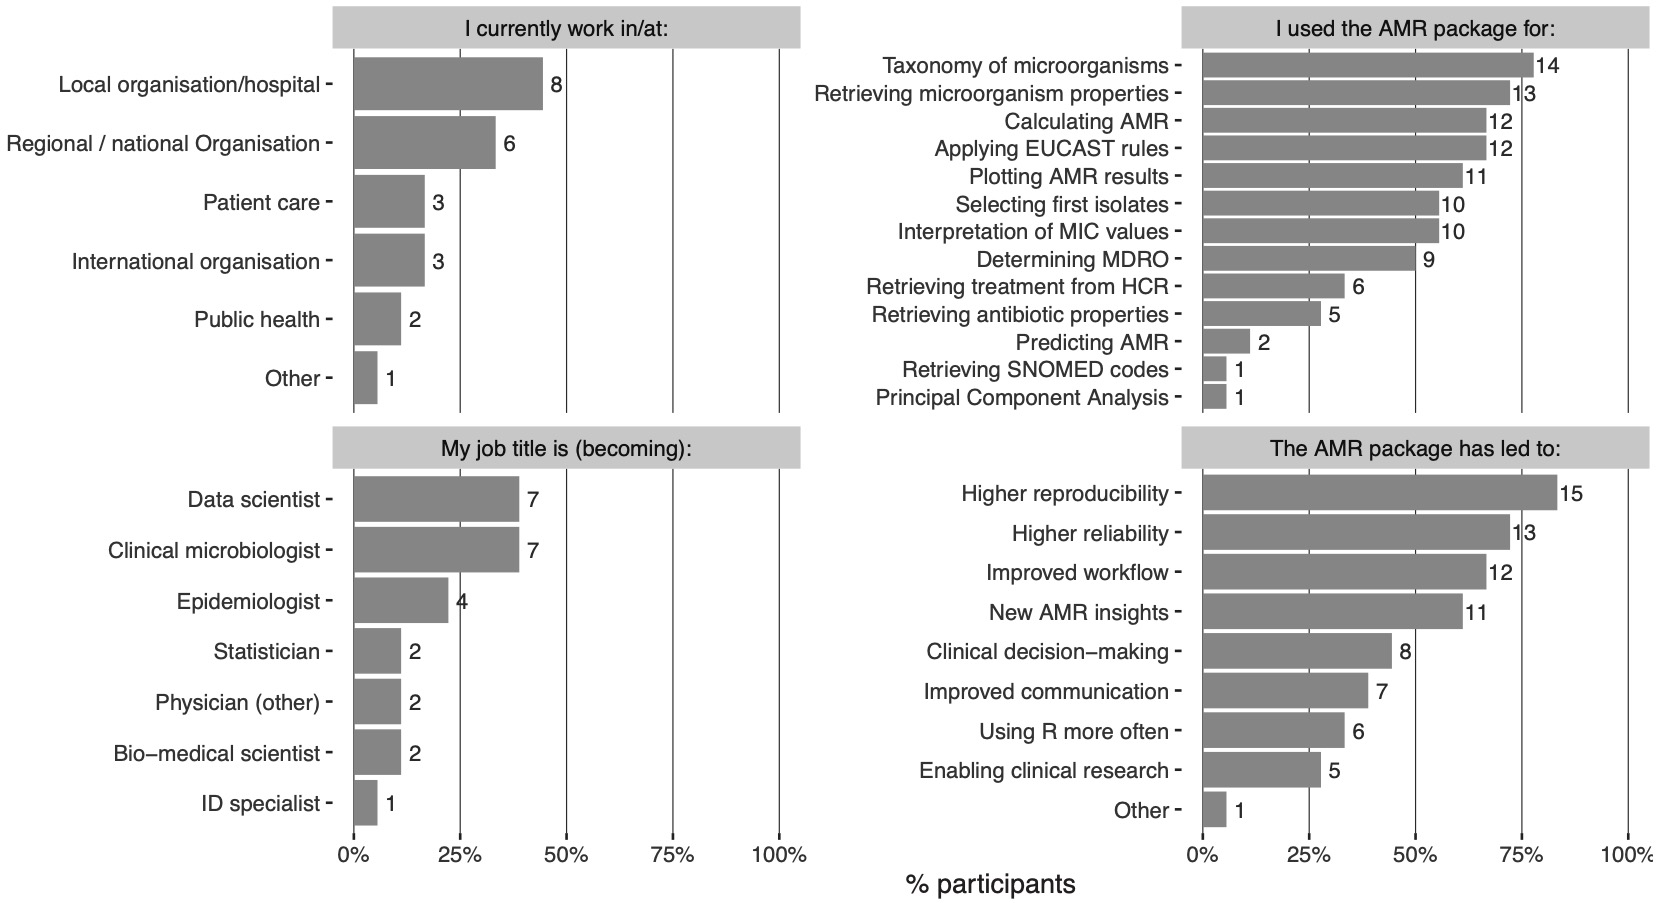
\includegraphics[width=1\linewidth]{images/03-02} 

}

\caption{The outcome of the survey amongst 18 participants. MIC: minimal inhibitory concentration, MDRO: multidrug-resistant organism, SNOMED: Systematised Nomenclature of Medicine.}\label{fig:fig3-2}
\end{figure}

Aside from AMR data analysis, most participants (78\%) used the AMR package as a reference for the taxonomy of microorganisms. It was also regularly used for interpreting raw MIC and disk diffusion values (56\%) and applying EUCAST expert rules (67\%). This is in line with the original aims of the AMR package development.

\hypertarget{conclusion-1}{%
\section{Conclusion}\label{conclusion-1}}

AMR data analysis is dependent on (inter-)national guidelines and reliable (reference) data on the one hand but constrained by diverse and often inadequate data analysis tools and poor data quality on the other. We aimed to address these dependencies and constraints by introducing the AMR package for R for standardised and reproducible AMR data analyses. Our first insights into the usage and the usability of the AMR package confirm that this package is fulfilling its intended aim. Regional, national, and international organisations already use the AMR package to support clinical decision-making in infection management by gaining new or improved insights into resistance levels. We invite others to make use of our open-source approach and adapt it to their needs. The advantages of sharing open-source software such as the AMR package allow for a collaborative, transparent use and further development that can lead to more standardised analysis processes for AMR data. The flexible open-source design also enables rapid integration of updated guidelines (e.g., new EUCAST breakpoints), and setting-specific adaptations are encouraged. Together, the AMR package for R can thus empower any specialist in the field working with AMR data by providing a comprehensive toolbox of solutions for AMR data analysis.

\hypertarget{references-2}{%
\section*{References}\label{references-2}}
\addcontentsline{toc}{section}{References}

\begin{enumerate}
\def\labelenumi{\arabic{enumi}.}
\tightlist
\item
  Limmathurotsakul D, Dunachie S, Fukuda K, Feasey NA, Okeke IN, Holmes AH, \emph{et al.} Improving the estimation of the global burden of antimicrobial resistant infections. Lancet Infect Dis 2019;3099:1--7. \url{doi:10.1016/S1473-3099(19)30276-2}.
\item
  OECD. Stemming the Superbug Tide. Paris: OECD; 2018. \url{doi:10.1787/9789264307599-en}.
\item
  Hindler JF, Stelling J. Analysis and Presentation of Cumulative Antibiograms: A New Consensus Guideline from the Clinical and Laboratory Standards Institute. Clin Infect Dis 2007;44:867--73. \url{doi:10.1086/511864}.
\item
  Brown D, Canton R, Dubreuil L, Gatermann S, Giske C, MacGowan A, \emph{et al.} Widespread implementation of EUCAST breakpoints for antibacterial susceptibility testing in Europe. Euro Surveill 2015;20. \url{doi:10.2807/1560-7917.es2015.20.2.21008}.
\item
  EUCAST. The European Committee on Antimicrobial Susceptibility Testing. Breakpoint tables for interpretation of MICs and zone diameters. Version 10.0. 2020.
\item
  Kassim A, Omuse G, Premji Z, Revathi G. Comparison of Clinical Laboratory Standards Institute and European Committee on Antimicrobial Susceptibility Testing guidelines for the interpretation of antibiotic susceptibility at a University teaching hospital in Nairobi, Kenya: a cross-sectional stud. Ann Clin Microbiol Antimicrob 2016;15:21. \url{doi:10.1186/s12941-016-0135-3}.
\item
  Kassim A, Pflüger V, Premji Z, Daubenberger C, Revathi G. Comparison of biomarker based Matrix Assisted Laser Desorption Ionization-Time of Flight Mass Spectrometry (MALDI-TOF MS) and conventional methods in the identification of clinically relevant bacteria and yeast. BMC Microbiol 2017;17:128. \url{doi:10.1186/s12866-017-1037-z}.
\item
  Parte AC, Sardà Carbasse J, Meier-Kolthoff JP, Reimer LC, Göker M. List of Prokaryotic names with Standing in Nomenclature (LPSN) moves to the DSMZ. Int J Syst Evol Microbiol 2020;70:5607--12. \url{doi:10.1099/ijsem.0.004332}.
\item
  Tindall BJ, Sutton G, Garrity GM. \emph{Enterobacter aerogenes} Hormaeche and Edwards 1960 (Approved Lists 1980) and \emph{Klebsiella mobilis} Bascomb \emph{et al.} 1971 (Approved Lists 1980) share the same nomenclatural type (ATCC 13048) on the Approved Lists and are homotypic synonyms, with consequences for. Int J Syst Evol Microbiol 2017;67:502--4. \url{doi:10.1099/ijsem.0.001572}.
\item
  Alnajar S, Gupta RS. Phylogenomics and comparative genomic studies delineate six main clades within the family \emph{Enterobacteriaceae} and support the reclassification of several polyphyletic members of the family. Infect Genet Evol 2017;54:108--27. \url{doi:10.1016/j.meegid.2017.06.024}.
\item
  Berends MS, Luz CF, Friedrich AW, Sinha BNM, Albers CJ, Glasner C. AMR - An R Package for Working with Antimicrobial Resistance Data. J Stat Softw 2021;(in press). \url{doi:https://doi.org/10.1101/810622}.
\item
  EUCAST. The European Committee on Antimicrobial Susceptibility Testing. Intrinsic Resistance and Exceptional Phenotypes. Version 3.1. 2016.
\item
  EUCAST. The European Committee on Antimicrobial Susceptibility Testing. Intrinsic Resistance and Exceptional Phenotypes. Version 3.2. 2020.
\item
  Le Guern R, Titécat M, Loïez C, Duployez C, Wallet F, Dessein R. Comparison of time-to-positivity between two blood culture systems: a detailed analysis down to the genus-level. Eur J Clin Microbiol Infect Dis 2021. \url{doi:10.1007/s10096-021-04175-9}.
\item
  Dutey-Magni PF, Gill MJ, McNulty D, Sohal G, Hayward A, Shallcross L, \emph{et al.} Feasibility study of hospital antimicrobial stewardship analytics using electronic health records. JAC-Antimicrobial Resist 2021;3. \url{doi:10.1093/jacamr/dlab018}.
\item
  N. Tenea G, Jarrin-V P, Yepez L. Microbiota of Wild Fruits from the Amazon Region of Ecuador: Linking Diversity and Functional Potential of Lactic Acid Bacteria with Their Origin. Ecosyst. Biodivers. Amaz., IntechOpen; 2021. \url{doi:10.5772/intechopen.94179}.
\item
  Kim S, Yoo SJ, Chang J. Importance of Susceptibility Rate of `the First' Isolate: Evidence of Real-World Data. Medicina (B Aires) 2020;56:507. \url{doi:10.3390/medicina56100507}.
\item
  World Health Organization. WHONET 2020. \url{https://whonet.org} (accessed May 20, 2021).
\item
  Centers for Disease Control and Prevention (CDC). Epi Info (TM) 2020. \url{https://www.cdc.gov/epiinfo/index.html} (accessed May 20, 2021).
\end{enumerate}

\hypertarget{ch04-amr-r-package}{%
\chapter{\texorpdfstring{\texttt{AMR} - An \texttt{R} Package for Working with Antimicrobial Resistance Data}{AMR - An R Package for Working with Antimicrobial Resistance Data}}\label{ch04-amr-r-package}}

Accepted in Journal of Statistical Software (ahead of print)

(as of date of PhD defence: 25 August 2021)

Berends MS \textsuperscript{1,2}*, Luz CF \textsuperscript{2}*, Friedrich AW \textsuperscript{2}, Sinha BNM \textsuperscript{2}, Albers CJ \textsuperscript{3}, Glasner C \textsuperscript{2}

\begin{enumerate}
\def\labelenumi{\arabic{enumi}.}
\tightlist
\item
  Certe Medical Diagnostics and Advice Foundation, Groningen, the Netherlands
\item
  University of Groningen, University Medical Center Groningen, Department of Medical Microbiology and Infection Prevention, Groningen, the Netherlands
\item
  University of Groningen, Heymans Institute for Psychological Research, Groningen, the Netherlands
\end{enumerate}

* These authors contributed equally

\hypertarget{abstract-2}{%
\section*{Abstract}\label{abstract-2}}
\addcontentsline{toc}{section}{Abstract}

Antimicrobial resistance is an increasing threat to global health. Evidence for this trend is generated in microbiological laboratories through testing microorganisms for resistance against antimicrobial agents. International standards and guidelines are in place for this process as well as for reporting data on (inter-)national levels. However, there is a gap in the availability of standardised and reproducible tools for working with laboratory data to produce the required reports. It is known that extensive efforts in data cleaning and validation are required when working with data from laboratory information systems. Furthermore, the global spread and relevance of antimicrobial resistance demands to incorporate international reference data in the analysis process. In this paper, we introduce the \texttt{AMR} package for\texttt{R} that aims at closing this gap by providing tools to simplify antimicrobial resistance data cleaning and analysis, while incorporating international guidelines and scientifically reliable reference data. The \texttt{AMR} package enables standardised and reproducible antimicrobial resistance analyses, including the application of evidence-based rules, determination of first isolates, translation of various codes for microorganisms and antimicrobial agents, determination of (multi-drug) resistant microorganisms, and calculation of antimicrobial resistance, prevalence and future trends. The \texttt{AMR} package works independently of any laboratory information system and provides several functions to integrate into international workflows (e.g., WHONET software provided by the World Health Organization).

\hypertarget{introduction-1}{%
\section{Introduction}\label{introduction-1}}

Antimicrobial resistance is a global health problem and of great concern for human medicine, veterinary medicine, and the environment alike. It is associated with significant burdens to both patients and health care systems. Current estimates show the immense dimensions we are already facing, such as claiming at least 50,000 lives due to antimicrobial resistance each year across Europe and the US alone \textsuperscript{{[}1{]}}. Although estimates for the burden through antimicrobial resistance and their predictions are disputed \textsuperscript{{[}2{]}} the rising trend is undeniable \textsuperscript{{[}3{]}}, thus calling for worldwide efforts on tackling this problem.

Surveillance programs and reliable data are key for controlling and streamlining these efforts. Surveillance data of antimicrobial resistance at higher levels (national or international) usually comprise aggregated numbers. The basis of this information is generated and stored at local microbiological laboratories where isolated microorganisms are tested for their susceptibility to a whole range of antimicrobial agents. The efficacy of these agents against microorganisms is nowadays interpreted as follows \textsuperscript{{[}4{]}}:

\begin{itemize}
\tightlist
\item
  R (``resistant'') - there is a high likelihood of therapeutic failure;
\item
  S (``susceptible, standard dosing regimen'') - there is a high likelihood of therapeutic success using a standard dosing regimen of an antimicrobial agent;
\item
  I (``susceptible, increased exposure'') - there is a high likelihood of therapeutic success, but only when exposure to an antimicrobial agent is increased by adjusting the dosing regimen or its concentration at the site of infection.
\end{itemize}

Generally, antimicrobial resistance is defined as the proportion of resistant microorganisms (R) among all tested microorganisms of the same species (R + S + I). Today, the two major guideline institutes to define the international standards on antimicrobial resistance are the European Committee on Antimicrobial Susceptibility Testing (EUCAST) \textsuperscript{{[}5{]}} and the Clinical and Laboratory Standards Institute (CLSI) \textsuperscript{{[}6{]}}. The guidelines from these two institutes are adopted by 94\% of all countries reporting antimicrobial resistance to the WHO \textsuperscript{{[}7{]}}.

Although these standardised guidelines are in place on the laboratory level for the data generation process, stored data in laboratory information systems are often not yet suitable for data analysis. Laboratory information systems are often designed to fit billing purposes rather than epidemiological data analysis. Furthermore, (inter-)national surveillance is hindered by inadequate standardisation of epidemiological definitions, different types of samples and data collection, settings included, microbiological testing methods (including susceptibility testing), and data sharing policies \textsuperscript{{[}8{]}}. The necessity of accurate data analysis in the field of antimicrobial resistance has just recently been further underlined \textsuperscript{{[}9{]}}. Antimicrobial resistance analyses require a thorough understanding of microbiological tests and their results, the biological taxonomy of microorganisms, the clinical and epidemiological relevance of the results, their pharmaceutical implications, and (inter-)national standards and guidelines for working with and reporting antimicrobial resistance.

Here, we describe the \texttt{AMR} package for\texttt{R} \textsuperscript{{[}10{]}}, which has been developed to standardise clean and reproducible antimicrobial resistance data analyses using international standardised recommendations \textsuperscript{{[}5,6{]}} while incorporating scientifically reliable reference data about valid laboratory outcome, antimicrobial agents, and the complete biological taxonomy of microorganisms. The \texttt{AMR} package provides solutions and support for these aspects while being independent of underlying laboratory information systems, thereby democratising the analysis process. Developed in\texttt{R} and available on the Comprehensive\texttt{R} Archive Network (CRAN) since February 22nd 2018 \textsuperscript{{[}11{]}}, the \texttt{AMR} package enables reproducible workflows as described in other fields, such as environmental science \textsuperscript{{[}12{]}}. The \texttt{AMR} package provides a new technical instrument to aid in curbing the global threat of antimicrobial resistance. Furthermore, local, and regional data in the laboratories can now become relevant in any setting for public health.

While no other packages\texttt{R} package with the purpose of dealing with antimicrobial resistance data are available on CRAN or Bioconductor, the \texttt{AMR} package may be integrated in workflows of related packages. For example, the\texttt{R} Epidemics Consortium (RECON) provides high-quality packages for data analysis in infectious disease outbreaks or epidemics (for example incidence and epicontacts) \textsuperscript{{[}13,14{]}}. In addition, on the laboratory side the antibioticR package provides approaches to work with disc diffusion zone diameter and minimum inhibitory concentration data from environment samples \textsuperscript{{[}15{]}}. We aim at providing a comprehensive and standardised toolbox for antimicrobial resistance data processing and analysis, with a focus on microbiological, clinical, and epidemiological purposes that was yet missing.

The following sections describe the functionality of the \texttt{AMR} package according to its core functionalities for transforming, enhancing, and analysing antimicrobial resistance data using scientifically reliable reference data.

\hypertarget{antimicrobial-resistance-data}{%
\section{Antimicrobial resistance data}\label{antimicrobial-resistance-data}}

Microbiological tests can be performed on different specimens, such as blood or urine samples or nasal swabs. After arrival at the microbiological laboratory, the specimens are traditionally cultured on specific media, such as blood agar. If a microorganism can be isolated from these media, it is tested against several antimicrobial agents. Based on the minimal inhibitory concentration (MIC) of the respective agent and interpretation guidelines, such as guidelines by EUCAST \textsuperscript{{[}5{]}} and CLSI \textsuperscript{{[}6{]}}, test results are reported as ``resistant'' (R), ``susceptible'' (S) or ``susceptible, increased exposure'' (I). A typical data structure is illustrated in Table 1 \textsuperscript{{[}5{]}}.

Table 1. Example of an antimicrobial resistance report.

\begin{figure}

{\centering 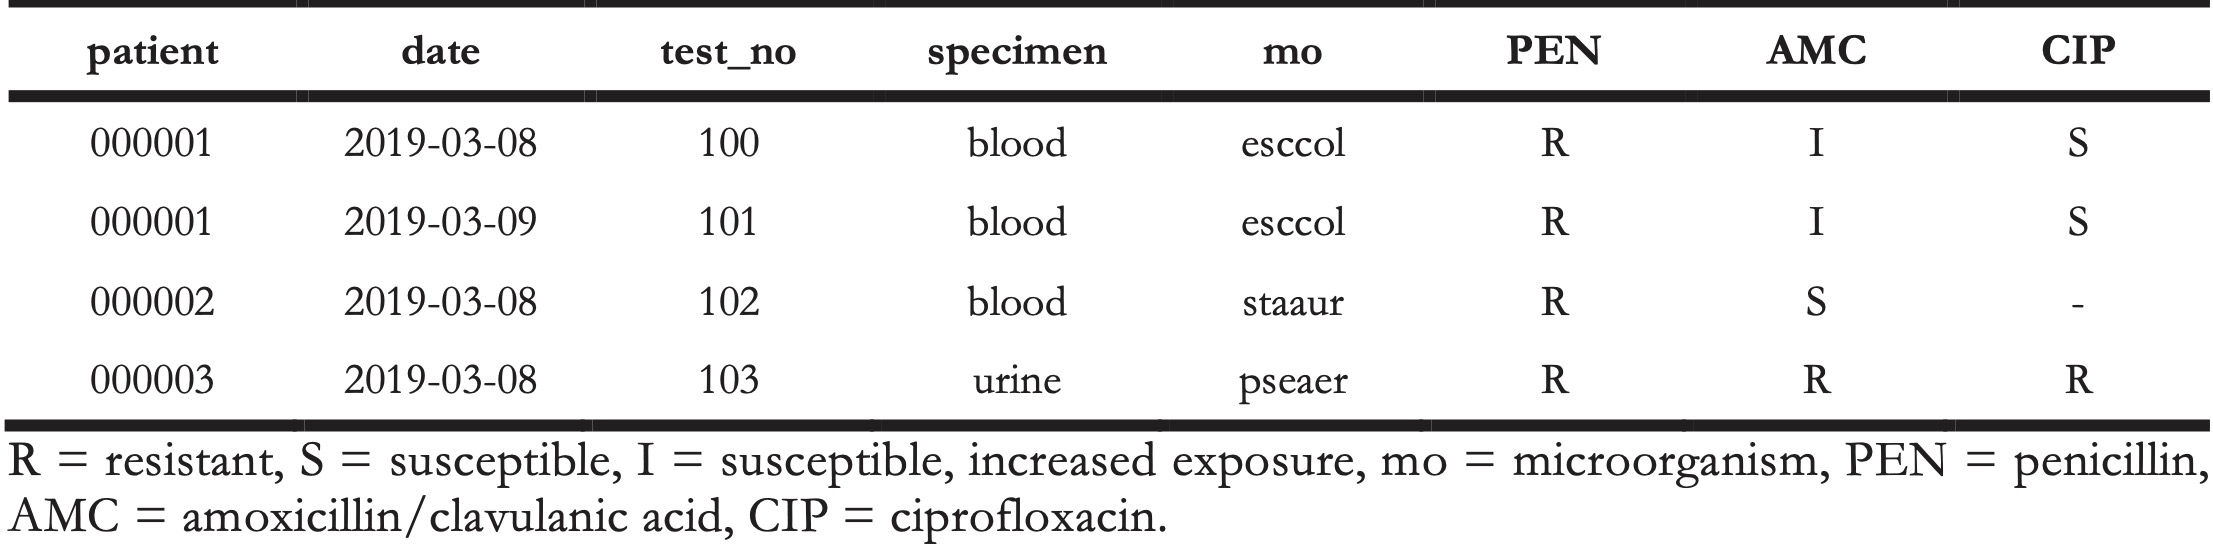
\includegraphics[width=1\linewidth]{images/04-t01} 

}

\end{figure}

Table 2. Example of an antimicrobial resistance report.

\begin{figure}

{\centering 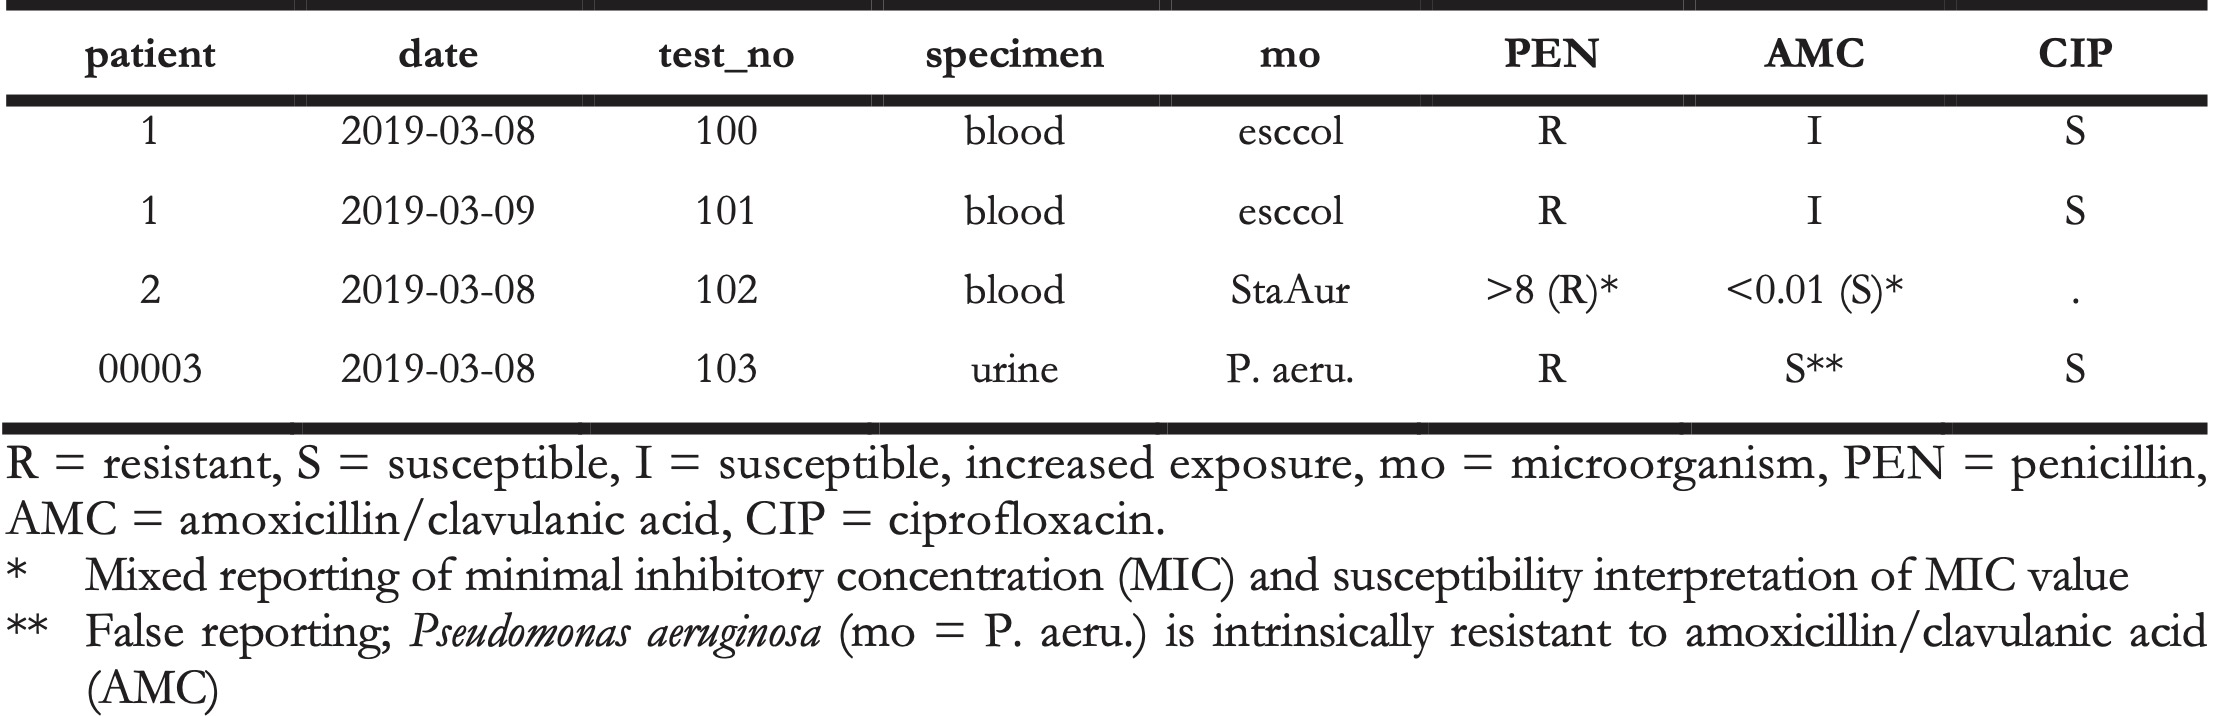
\includegraphics[width=1\linewidth]{images/04-t02} 

}

\end{figure}

The \texttt{AMR} package aims at providing a standardised and automated way of cleaning, transforming, and enhancing these typical data structures (Table 1 and 2), independent of the underlying data source. Processed data would be similar to Table 3 that highlights several package functionalities in the sections below.

Table 3. Enhanced antimicrobial resistance report example.

\begin{figure}

{\centering 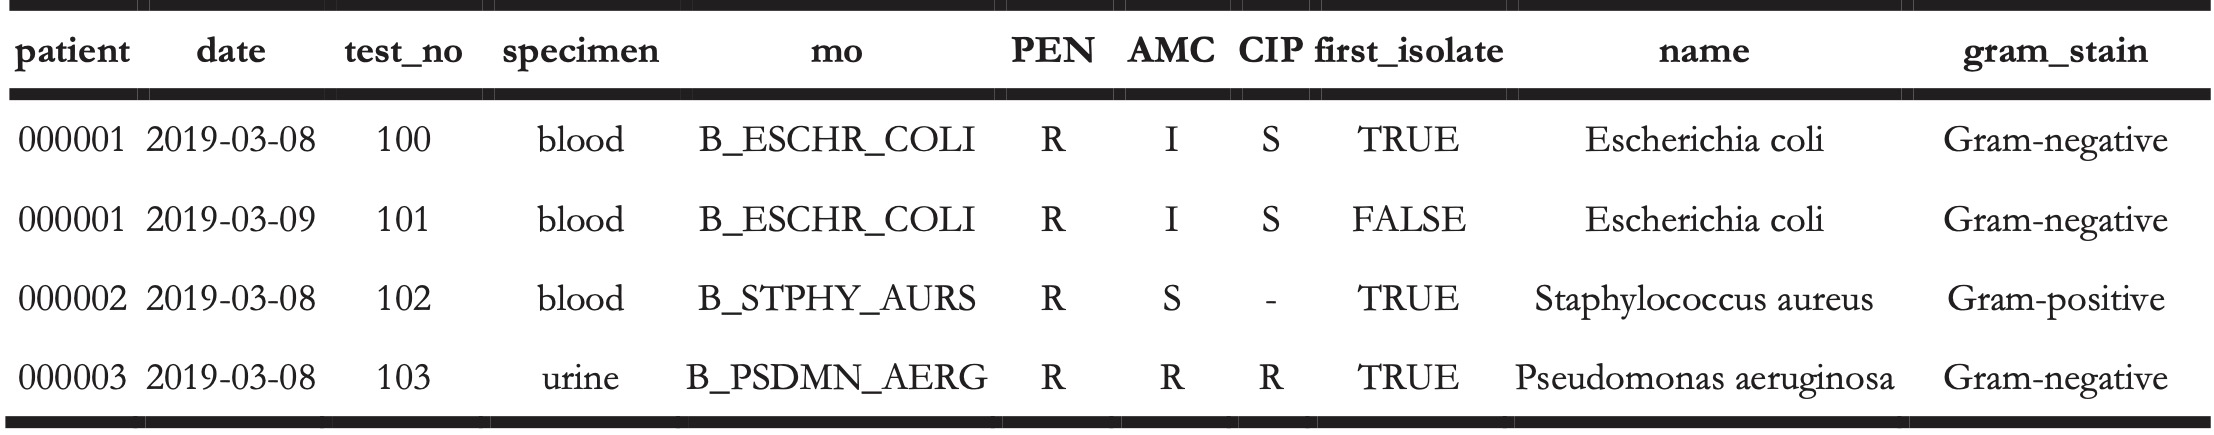
\includegraphics[width=1\linewidth]{images/04-t03} 

}

\end{figure}

\hypertarget{antimicrobial-resistance-data-transformation}{%
\section{Antimicrobial resistance data transformation}\label{antimicrobial-resistance-data-transformation}}

\hypertarget{working-with-taxonomically-valid-microorganism-names}{%
\subsection{Working with taxonomically valid microorganism names}\label{working-with-taxonomically-valid-microorganism-names}}

Coercing is a computational process of forcing output based on an input. For microorganism names, coercing user input to taxonomically valid microorganism names is crucial to ensure correct interpretation and to enable grouping based on taxonomic properties. To this end, the \texttt{AMR} package includes all microbial entries from The Catalogue of Life (\url{http://www.catalogueoflife.org}), the most comprehensive and authoritative global index of species currently available \textsuperscript{{[}16{]}}. It holds essential information on the names, relationships, and distributions of more than 1.9 million species. The integration of it into the \texttt{AMR} package is described in Appendix A.

The \texttt{as.mo()} function makes use of this underlying data to transform a vector of characters to a new class `\texttt{‘mo’} of taxonomically valid microorganism name. The resulting values are microbial IDs, which are human-readable for the trained eye and contain information about the taxonomic kingdom, genus, species, and subspecies (Figure 1).

\begin{figure}

{\centering 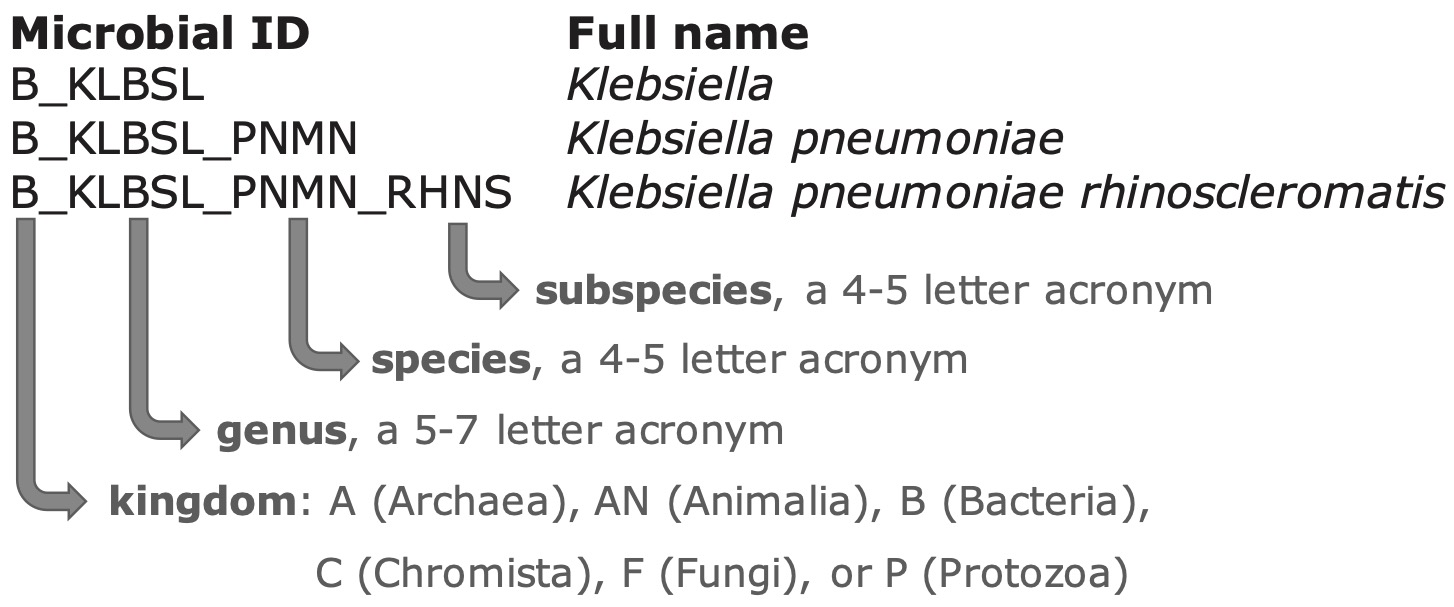
\includegraphics[width=0.66\linewidth]{images/04-01} 

}

\caption{The structure of a typical microbial ID as used in the `AMR` package. An ID consists of two to four elements, separated by an underscore. The first element is the abbreviation of the taxonomic kingdom. The remaining elements consist of abbreviations of the lowest taxonomic levels of every microorganism: genus, species (if available) and subspecies (if available). Abbreviations used for the microbial IDs of microorganism names were created using the base` R` function `abbreviate()`.}\label{fig:fig4-1}
\end{figure}

The \texttt{as.mo()} function compares the user input with taxonomically valid microorganism names, rates the matching with a score and returns results based on the highest score. This matching score (\(m\)), ranging from \(0\) to \(1\), is calculated using the following equation:

\[m_{(x,n)} = \frac{l_{n} - 0.5 \cdot \min\{ l_n, \operatorname{lev}(x,n) \} }{l_{n} \cdot p_{n} \cdot k_{n}}\]

where:

\begin{itemize}
\tightlist
\item
  \(x\) is the user input;
\item
  \(n\) is a taxonomic name (genus, species, and subspecies);
\item
  \(l_n\) is the length of \(n\);
\item
  lev is the Levenshtein distance function \textsuperscript{{[}17{]}}, which counts any insertion, deletion and substitution as \(1\) that is needed to change \(x\) into \(n\);
\item
  \(p_n\) is the human pathogenic prevalence group of \(n\), as described below;
\item
  \(k_n\) is the taxonomic kingdom of \(n\), set as Bacteria = 1, Fungi = 2, Protozoa = 3, Archaea = 4, others = 5.
\end{itemize}

The grouping into human pathogenic prevalence (\(p\)) is based on experience from several microbiological laboratories in the Netherlands in conjunction with international reports on pathogen prevalence \textsuperscript{{[}7,18,19{]}}. \textbf{Group 1} (most prevalent microorganisms) consists of all microorganisms where the taxonomic class is Gammaproteobacteria or where the taxonomic genus is \emph{Enterococcus}, \emph{Staphylococcus} or \emph{Streptococcus}. This group consequently contains all common Gram-negative bacteria, such as \emph{Pseudomonas} and \emph{Legionella} and all species within the order Enterobacterales. \textbf{Group 2} consists of all microorganisms where the taxonomic phylum is Proteobacteria, Firmicutes, Actinobacteria or Sarcomastigophora, or where the taxonomic genus is \emph{Absidia}, \emph{Acremonium}, \emph{Actinotignum}, \emph{Alternaria}, \emph{Anaerosalibacter}, \emph{Apophysomyces}, \emph{Arachnia}, \emph{Aspergillus}, \emph{Aureobacterium}, \emph{Aureobasidium}, \emph{Bacteroides}, \emph{Basidiobolus}, \emph{Beauveria}, \emph{Blastocystis}, \emph{Branhamella}, \emph{Calymmatobacterium}, \emph{Candida}, \emph{Capnocytophaga}, \emph{Catabacter}, \emph{Chaetomium}, \emph{Chryseobacterium}, \emph{Chryseomonas}, \emph{Chrysonilia}, \emph{Cladophialophora}, \emph{Cladosporium}, \emph{Conidiobolus}, \emph{Cryptococcus}, \emph{Curvularia}, \emph{Exophiala}, \emph{Exserohilum}, \emph{Flavobacterium}, \emph{Fonsecaea}, \emph{Fusarium}, \emph{Fusobacterium}, \emph{Hendersonula}, \emph{Hypomyces}, \emph{Koserella}, \emph{Lelliottia}, \emph{Leptosphaeria}, \emph{Leptotrichia}, \emph{Malassezia}, \emph{Malbranchea}, \emph{Mortierella}, \emph{Mucor}, \emph{Mycocentrospora}, \emph{Mycoplasma}, \emph{Nectria}, \emph{Ochroconis}, \emph{Oidiodendron}, \emph{Phoma}, \emph{Piedraia}, \emph{Pithomyces}, \emph{Pityrosporum}, \emph{Prevotella}, \emph{Pseudallescheria}, \emph{Rhizomucor}, \emph{Rhizopus}, \emph{Rhodotorula}, \emph{Scolecobasidium}, \emph{Scopulariopsis}, \emph{Scytalidium}, \emph{Sporobolomyces}, \emph{Stachybotrys}, \emph{Stomatococcus}, \emph{Treponema}, \emph{Trichoderma}, \emph{Trichophyton}, \emph{Trichosporon}, \emph{Tritirachium} or \emph{Ureaplasma}. \textbf{Group 3} consists of all other microorganisms.

This will lead to the effect that e.g., \texttt{"E.\ coli"} will return the microbial ID of \emph{Escherichia coli} (\(m = 0.688\), a highly prevalent microorganism found in humans) and not \emph{Entamoeba coli} (\(m = 0.079\), a less prevalent microorganism in humans), although the latter would alphabetically come first. The matching score function is for users available as \texttt{mo\_matching\_score()}.

If any coercion rules are applied, a warning is printed to the console and scores can be reviewed by calling \texttt{mo\_uncertainties()}, that prints all other matches with their matching scores. Users can furthermore control the coercion rules by setting the allow\_uncertain argument in the \texttt{as.mo()} function. The following values or levels can be used:

\begin{itemize}
\tightlist
\item
  \texttt{0}: no additional rules are applied;
\item
  \texttt{1}: allow previously accepted (but now invalid) taxonomic names and minor spelling errors;
\item
  \texttt{2}: allow all of 1, strip values between brackets, inverse the words of the input, strip off text elements from the end keeping at least two elements;
\item
  \texttt{3}: allow all of level 1 and 2, strip off text elements from the end, allow any part of a taxonomic name;
\item
  \texttt{TRUE} (default): equivalent to \texttt{2};
\item
  \texttt{FALSE}: equivalent to \texttt{0}.
\end{itemize}

To support organisation specific microbial IDs, users can specify a custom reference \texttt{‘data.frame’}, by using \texttt{as.mo(...,\ reference\_df\ =\ ...)}. This process can also be automated by users with the \texttt{set\_mo\_source()} function.

\hypertarget{properties-of-microorganisms}{%
\subsubsection{Properties of microorganisms}\label{properties-of-microorganisms}}

The package contains functions to return a specific (taxonomic) property of a microorganism from the \texttt{microorganisms} data set (see Appendix A). Functions that start with \texttt{mo\_*} can be used to retrieve the most recently defined taxonomic properties of any microorganism quickly and conveniently. These functions rely on the \texttt{as.mo()} function internally: \texttt{mo\_name()}, \texttt{mo\_fullname()}, \texttt{mo\_shortname()}, \texttt{mo\_subspecies()}, \texttt{mo\_species()}, \texttt{mo\_genus()}, \texttt{mo\_family()}, \texttt{mo\_order()}, \texttt{mo\_class()}, \texttt{mo\_phylum()}, \texttt{mo\_kingdom()}, \texttt{mo\_type()}, \texttt{mo\_gramstain()}, \texttt{mo\_ref()}, \texttt{mo\_authors()}, \texttt{mo\_year()}, \texttt{mo\_rank()}, \texttt{mo\_taxonomy()}, \texttt{mo\_synonyms()}, \texttt{mo\_info()} and \texttt{mo\_url()}. Determination of the Gram stain, by using \texttt{mo\_gramstain()}, is based on the taxonomic subkingdom and phylum. According to Cavalier-Smith \textsuperscript{{[}20{]}}, who defined the subkingdoms Negibacteria and Posibacteria, only the following phyla are Posibacteria: Actinobacteria, Chloroflexi, Firmicutes and Tenericutes. Bacteria from these phyla are considered Gram-positive - all other bacteria are considered Gram-negative. Gram stains are only relevant for species within the kingdom of Bacteria. For species outside this kingdom, \texttt{mo\_gramstain()} will return \texttt{NA}.

\hypertarget{working-with-antimicrobial-names-or-codes}{%
\subsection{Working with antimicrobial names or codes}\label{working-with-antimicrobial-names-or-codes}}

The \texttt{AMR} package includes the \texttt{antibiotics} data set, which comprises common laboratory information system codes, official names, ATC (Anatomical Therapeutic Chemical) codes, defined daily doses (DDD) and more than 5,000 trade names of 456 antimicrobial agents (see Appendix A). The ATC code system and the reference list for DDDs have been developed and made available by the World Health Organization Collaborating Centre for Drug Statistics Methodology (WHOCC) to standardise pharmaceutical classifications \textsuperscript{{[}21{]}}. All agents in the \texttt{antibiotics} data set have a unique antimicrobial ID, which is based on abbreviations used by the European Antimicrobial Resistance Surveillance Network (EARS-Net), the largest publicly funded system for antimicrobial resistance surveillance in Europe \textsuperscript{{[}22{]}}. Furthermore, the \texttt{AMR} package includes the antivirals data seta containing antiviral agents, which is also described in Appendix A.

\hypertarget{properties-of-antimicrobial-agents}{%
\subsubsection{Properties of antimicrobial agents}\label{properties-of-antimicrobial-agents}}

It is a common task in microbiological data analyses (and other clinical or epidemiological fields) to work with different antimicrobial agents. The \texttt{AMR} package provides several functions to translate inputs such as ATC codes, abbreviations, or names in any direction. Using \texttt{as.ab()}, any input will be transformed to an antimicrobial ID of class \texttt{‘ab’}. Helper functions are available to get specific properties of antimicrobial IDs, such as \texttt{ab\_name()} for getting the official name, \texttt{ab\_atc()} for the ATC code, or \texttt{ab\_cid()} for the CID (Compound ID) used by PubChem \textsuperscript{{[}23{]}}. Trade names can be also used as input. For example, the input values ``Amoxil'', ``dispermox'', ``amox'' and ``J01CA04'' all return the ID of amoxicillin (AMX):

\begin{Shaded}
\begin{Highlighting}[]
\FunctionTok{as.ab}\NormalTok{(}\StringTok{"Amoxicillin"}\NormalTok{)}
\CommentTok{\#\textgreater{} Class \textless{}ab\textgreater{}}
\CommentTok{\#\textgreater{} [1] AMX}

\FunctionTok{as.ab}\NormalTok{(}\FunctionTok{c}\NormalTok{(}\StringTok{"Amoxil"}\NormalTok{, }\StringTok{"dispermox"}\NormalTok{, }\StringTok{"amox"}\NormalTok{, }\StringTok{"J01CA04"}\NormalTok{))}
\CommentTok{\#\textgreater{} Class \textless{}ab\textgreater{}}
\CommentTok{\#\textgreater{} [1] AMX AMX AMX AMX}

\FunctionTok{ab\_name}\NormalTok{(}\StringTok{"Amoxil"}\NormalTok{)}
\CommentTok{\#\textgreater{} [1] "Amoxicillin" }

\FunctionTok{ab\_atc}\NormalTok{(}\StringTok{"amox"}\NormalTok{)}
\CommentTok{\#\textgreater{} [1] "J01CA04"}

\FunctionTok{ab\_name}\NormalTok{(}\StringTok{"J01CA04"}\NormalTok{)}
\CommentTok{\#\textgreater{} [1] "Amoxicillin"}
\end{Highlighting}
\end{Shaded}

If more than one antimicrobial agent is found in the input string, a warning with the additional findings is printed to the console.

\hypertarget{filtering-data-based-on-classes-of-antimicrobial-agents}{%
\subsubsection{Filtering data based on classes of antimicrobial agents}\label{filtering-data-based-on-classes-of-antimicrobial-agents}}

The application of the ATC classification system also enables grouping of antimicrobial agents for data analyses. Data sets with microbial isolates can be filtered on isolates with specific results for tested antimicrobial agents in a specific antimicrobial class. For example, using \texttt{filter\_carbapenems(result\ =\ "R")} returns data of all isolates with tested resistance to any of the 14 available antimicrobial agents in in the group of carbapenems according to the \texttt{antibiotics} data set.

\hypertarget{working-with-antimicrobial-susceptibility-test-results}{%
\subsection{Working with antimicrobial susceptibility test results}\label{working-with-antimicrobial-susceptibility-test-results}}

Minimal inhibitory concentrations (MIC) are susceptibility test results measured by microbiological laboratory equipment to determine at which minimum antimicrobial drug concentration 99.9\% of a microorganism is inhibited in growth. These concentrations are often capped at a minimum and maximum, for example ≤0.02 µg/ml and ≥32 µg/ml, respectively. The \texttt{‘mic’} class, an ordered \texttt{‘factor’} containing valid MIC values, keeps these operators while still ordering all possible outcomes correctly so that e.g., ``\textless=0.02'' will be considered lower than ``0.04''.

Another susceptibility testing method is the use of drug diffusion disks, which are small tablets containing a specified concentration of an antimicrobial agent. These disks are applied onto a solid growth medium or a specific agar plate. After 24 hours of incubation, the diameter of the growth inhibition around a disk can be measured in millimetres with a ruler. The \texttt{‘disk’} class can be used to clean these kinds of measurements, since they should always be valid numeric values between 6 and 50. The supported minima and maxima of valid values for both classes, \texttt{‘mic’} and \texttt{‘disk’}, are displayed in Table 4.

Table 4. Antimicrobial susceptibility test classes.

\begin{figure}

{\centering 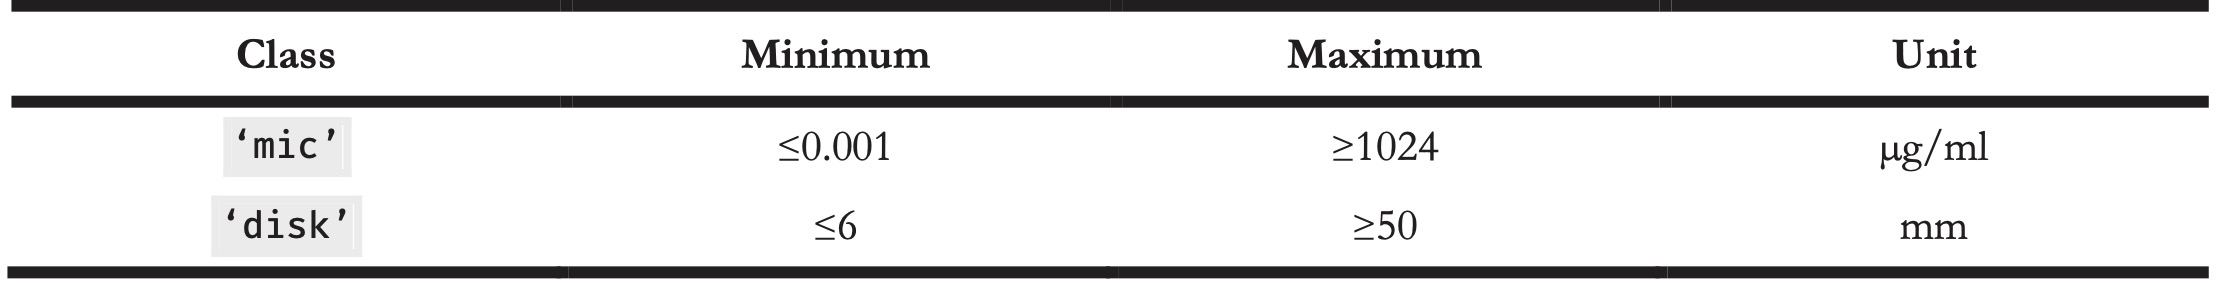
\includegraphics[width=1\linewidth]{images/04-t04} 

}

\end{figure}

The higher the MIC or the smaller the growth inhibition diameter, the more active substance of an antimicrobial agent is needed to inhibit cell growth, i.e.~the higher the antimicrobial resistance against the tested antimicrobial agent. At high MICs and small diameters, guidelines interpret the microorganism as ``resistant'' (R) to the tested antimicrobial agent. At low MICs and wide diameters, guidelines interpret the microorganism as ``susceptible'' (S) to the tested antimicrobial agent. In between, the microorganism is classified as ``susceptible, increased exposure'' (I). For these three interpretations the \texttt{‘rsi’} class has been developed. When using \texttt{as.rsi()} on MIC values (of class \texttt{‘mic’}) or disk diffusion diameters (of class \texttt{‘disk’}), the values will be interpreted according to the guidelines from the CLSI or EUCAST (all guidelines between 2011 and 2020 are included in the \texttt{AMR} package) \textsuperscript{{[}24,25{]}}. Guidelines can be changed by setting the guidelines argument.

\begin{Shaded}
\begin{Highlighting}[]
\CommentTok{\# Low MIC value}
\FunctionTok{as.rsi}\NormalTok{(}\FunctionTok{as.mic}\NormalTok{(}\DecValTok{2}\NormalTok{), }\StringTok{"E. coli"}\NormalTok{, }\StringTok{"ampicillin"}\NormalTok{, }\AttributeTok{guideline =} \StringTok{"EUCAST 2020"}\NormalTok{)}
\CommentTok{\#\textgreater{} Class \textless{}rsi\textgreater{}}
\CommentTok{\#\textgreater{} [1] S}

\CommentTok{\# High MIC value}
\FunctionTok{as.rsi}\NormalTok{(}\FunctionTok{as.mic}\NormalTok{(}\DecValTok{32}\NormalTok{), }\StringTok{"E. coli"}\NormalTok{, }\StringTok{"ampicillin"}\NormalTok{, }\AttributeTok{guideline =} \StringTok{"EUCAST 2020"}\NormalTok{)}
\CommentTok{\#\textgreater{} Class \textless{}rsi\textgreater{}}
\CommentTok{\#\textgreater{} [1] R}
\end{Highlighting}
\end{Shaded}

When using the \texttt{as.rsi()} function on existing antimicrobial interpretations, it tries to coerce the input to the values ``R'', ``S'' or ``I''. These values can in turn be used to calculate the proportion of antimicrobial resistance.

\hypertarget{interpretative-rules-by-eucast}{%
\subsection{Interpretative rules by EUCAST}\label{interpretative-rules-by-eucast}}

Next to supplying guidelines to interpret raw MIC values, EUCAST has developed a set of expert rules to assist clinical microbiologists in the interpretation and reporting of antimicrobial susceptibility tests \textsuperscript{{[}5{]}}. The rules comprise assistance on intrinsic resistance, exceptional phenotypes, and interpretive rules. The \texttt{AMR} package covers intrinsic resistant and interpretive rules for data transformation and standardisation purposes. The first prevents false susceptibility reporting by providing a list of organisms with known intrinsic resistance to specific antimicrobial agents (e.g., cephalosporin resistance of all enterococci). Interpretative rules apply inference from established resistance mechanisms \textsuperscript{{[}26-29{]}}. Both groups of rules are based on classic IF THEN statements (e.g., IF Enterococcus spp. resistant to ampicillin THEN also report as resistant to imipenem). Some rules provide assistance for further actions when certain resistance has been detected, i.e., performing additional testing of the isolated microorganism. The \texttt{AMR} package function \texttt{eucast\_rules()} can apply all EUCAST rules that do not rely on additional clinical information, such as additional information on patients' diagnoses. Table 2 and 3 highlight the transformation for the reporting of AMX = S in patient\_id = 000003 to the correct report according to EUCAST rules of AMX = R. Of note, however, EUCAST rules overwrite original data to correct for the difference in how antimicrobial agents affect the tested microorganism in vitro (in the laboratory) and in vivo (in the human body). This requires users to closely collaborate with the data source provider to ensure correct versioning, backward compatibility, reproducibility, and taking into account specific local regulation for resistance reporting. Typical scenarios where changes to the original data points apply include in vitro test results indicating susceptibility when resistance in vivo is known. The changes are based on scientific consensus to ensure reliable high-quality reporting of antimicrobial susceptibility results. All changes to the data are printed to the console and can also be reviewed in detail by setting the argument \texttt{eucast\_rules(...,\ verbose\ =\ TRUE)}.

EUCAST rules are subject to regular updates which are implemented into the \texttt{AMR} package by the \texttt{AMR} maintenance team shortly after publication. The \texttt{eucast\_rules()} function supports versioning of the rules. The arguments version\_breakpoints and version\_expertrules can be set to current or previous versions. By default, the \texttt{eucast\_rules()} function uses the latest implemented version.

\hypertarget{working-with-defined-daily-doses-ddd}{%
\subsection{Working with defined daily doses (DDD)}\label{working-with-defined-daily-doses-ddd}}

DDDs are essential for standardising antimicrobial consumption analysis, for inter-institutional or international comparison. The official DDDs are published by the WHOCC \textsuperscript{{[}36{]}}. Updates to the official publication are monitored by the \texttt{AMR} maintenance team and implemented in the \texttt{antibiotics} data set included in the \texttt{AMR} package. Other metrics exist such as the recommended daily dose (RDD) or the prescribed daily dose (PDD). However, DDDs are the only metric that is independent of a patient's disease and therapeutic choices and thus suitable for the \texttt{AMR} package.

Functions from the \texttt{atc\_online\_*()} family take any text as input that can be coerced with \texttt{as.ab()} (i.e., to class \texttt{‘ab’}). Next, the functions access the WHOCC online registry \textsuperscript{{[}30{]}} (internet connection required) and download the property defined in the arguments (e.g., administration = ``O'' or administration = ``P'' for oral or parenteral administration and property = ``ddd'' or property = ``groups'' to get DDD or the group of the selected antimicrobial defined by its ATC code).

\begin{Shaded}
\begin{Highlighting}[]
\FunctionTok{atc\_online\_ddd}\NormalTok{(}\StringTok{"amoxicillin"}\NormalTok{, }\AttributeTok{administration =} \StringTok{"O"}\NormalTok{)}
\CommentTok{\#\textgreater{} [1] 1.5}

\FunctionTok{atc\_online\_groups}\NormalTok{(}\StringTok{"amoxicillin"}\NormalTok{)}
\CommentTok{\#\textgreater{} [1] "ANTIINFECTIVES FOR SYSTEMIC USE"}
\CommentTok{\#\textgreater{} [2] "ANTIBACTERIALS FOR SYSTEMIC USE"}
\CommentTok{\#\textgreater{} [3] "BETA{-}LACTAM ANTIBACTERIALS, PENICILLINS"}
\CommentTok{\#\textgreater{} [4] "Penicillins with extended spectrum"}
\end{Highlighting}
\end{Shaded}

\hypertarget{enhancing-antimicrobial-resistance-data}{%
\section{Enhancing antimicrobial resistance data}\label{enhancing-antimicrobial-resistance-data}}

\hypertarget{determining-first-isolates}{%
\subsection{Determining first isolates}\label{determining-first-isolates}}

Determining antimicrobial resistance or susceptibility can be done for a single agent (mono- therapy) or multiple agents (combination therapy). The calculation of antimicrobial resistance statistics is dependent on two prerequisites: the data should only comprise the first isolates and a minimum required number of 30 isolates should be met for every stratum in further analysis \textsuperscript{{[}6{]}}.

An isolate is a microorganism strain cultivated on specified growth media in a laboratory, so its phenotype can be determined. First isolates are isolates of any species found first in a patient per episode, regardless of the body site or the type of specimen (such as blood or urine) \textsuperscript{{[}6{]}}. The selection on first isolates (using function \texttt{first\_isolate()}) is important to prevent selection bias, as it would lead to overestimated or underestimated resistance to an antimicrobial agent. For example, if a patient is admitted with a multi-drug resistant microorganism and that microorganism is found in five different blood cultures the following week, it would overestimate resistance if all isolates were to be included in the analysis.

The episode in days can be set with the argument episode\_days, which defaults to 365 as suggested by the CLSI guideline \textsuperscript{{[}6{]}}.

\hypertarget{determining-multi-drug-resistant-organisms-mdro}{%
\subsection{Determining multi-drug resistant organisms (MDRO)}\label{determining-multi-drug-resistant-organisms-mdro}}

Definitions of multi-drug resistant organisms (MDRO) are regulated by national and international expert groups and differ between nations. The \texttt{AMR} package provides the functionality to quickly identify MDROs in a data set using the \texttt{mdro()} function. Guidelines can be set with the argument guideline. At default, it applies the guideline as proposed by Magiorakos \emph{et al.} \textsuperscript{{[}31{]}}. Their work describes the definitions for bacteria being \texttt{‘MDR’} (multi-drug-resistant), \texttt{‘XDR’} (extensively drug-resistant) or \texttt{‘PDR’} (pan-drug-resistant). These definitions are widely adopted \textsuperscript{{[}32{]}} and known in the field of medical microbiology.

Other guidelines currently supported are the international EUCAST guideline (guideline = ``EUCAST'' \textsuperscript{{[}33{]}}), the international WHO guideline on the management of drug-resistant tuberculosis (guideline = ``TB'' \textsuperscript{{[}34{]}}), and the national guidelines of The Netherlands (guideline = ``NL'' \textsuperscript{{[}35{]}}), and Germany (guideline = ``DE'' \textsuperscript{{[}36{]}}).

Some guidelines require a minimum availability of tested antimicrobial agents per isolate. This is needed to prevent false-negatives, since no reliable determination can be performed on only a few test results. This required minimum defaults to 50\%, but can be set by the user with the pct\_minimum\_classes. Isolates that do not meet this requirement will be skipped for determination and will return \texttt{NA} (not applicable), with an informative warning printed to the console.

The rules are applied per row of the data. The \texttt{mdro()} function automatically identifies the variables containing the microorganism codes and antimicrobial agents based on the \texttt{guess\_ab\_col()} function. Following the guideline set by the user, it analyses the specific antimicrobial resistance of a microorganism and flags that microorganism accordingly. The outcome is demonstrated in Table 5, where the first row is an MDRO according to the Dutch guidelines \textsuperscript{{[}35{]}}.

Table 5. Example of a multi-drug resistant organism (MDRO) in a data set identified by applying Dutch guidelines.

\begin{figure}

{\centering 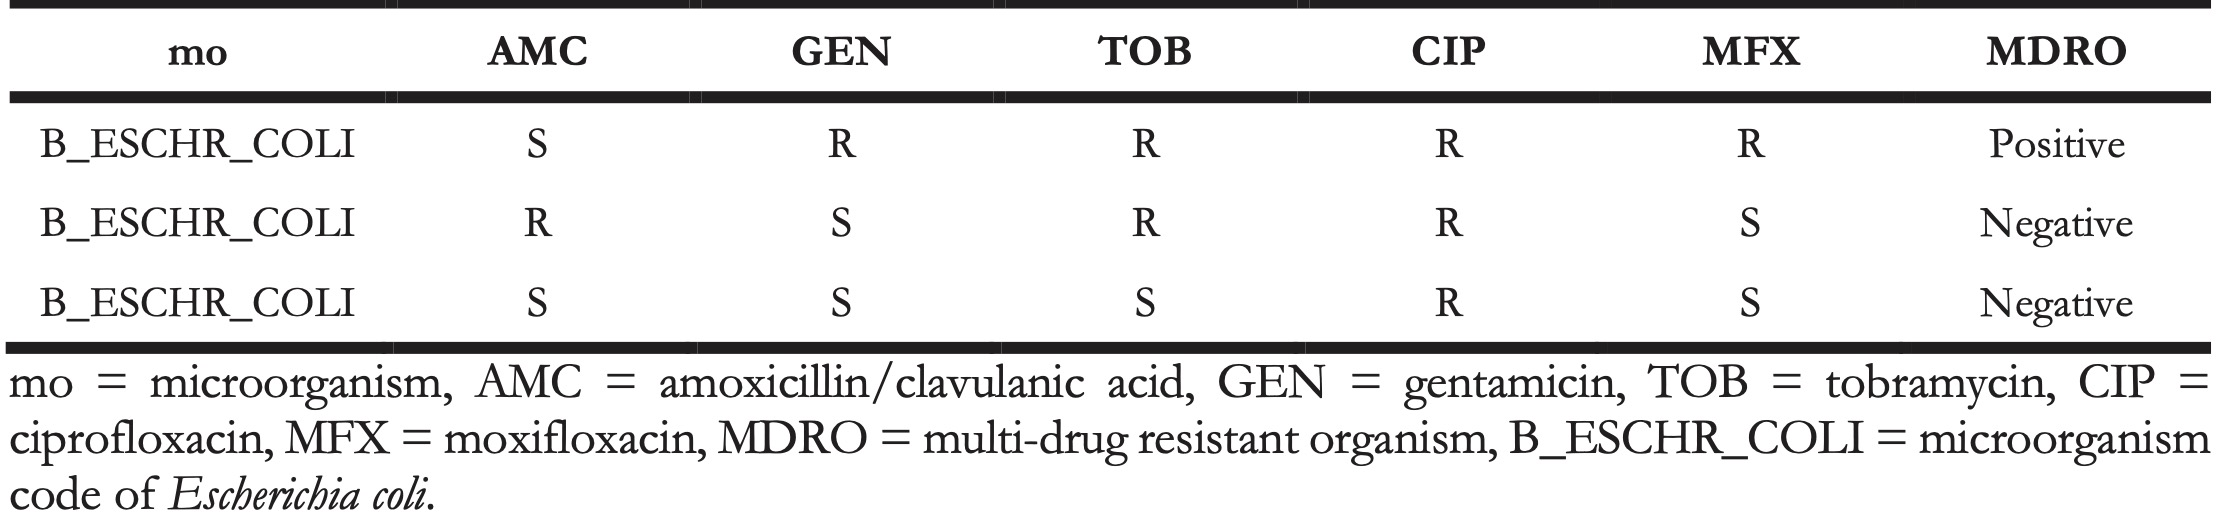
\includegraphics[width=1\linewidth]{images/04-t05} 

}

\end{figure}

\hypertarget{multi-drug-resistant-tuberculosis}{%
\subsubsection{Multi-drug resistant tuberculosis}\label{multi-drug-resistant-tuberculosis}}

Tuberculosis is a major threat to global health caused by Mycobacterium tuberculosis (MTB) and is one of the top ten causes of death worldwide \textsuperscript{{[}37{]}}. Exceptional antimicrobial resistance in MTB is therefore of special interest. To this end, the international WHO guideline for the classification of drug resistance in MTB \textsuperscript{{[}34{]}} is included in the \texttt{AMR} package. The \texttt{mdr\_tb()} function is a convenient wrapper around \texttt{mdro(...,\ guideline\ =\ "TB")}, which returns an other ordered \texttt{‘factor’} than other \texttt{mdro()} functions. The output will contain the \texttt{‘factor’} levels \texttt{‘Negative’} \textless{} \texttt{‘Mono-resistant’} \textless{} \texttt{‘Poly-resistant’} \textless{} \texttt{‘Multi-drug-resistant’} \textless{} \texttt{‘Extensively\ drug-resistant’}, following the WHO guideline.

\hypertarget{analysing-antimicrobial-resistance-data}{%
\section{Analysing antimicrobial resistance data}\label{analysing-antimicrobial-resistance-data}}

\hypertarget{calculation-of-antimicrobial-resistance}{%
\subsection{Calculation of antimicrobial resistance}\label{calculation-of-antimicrobial-resistance}}

The \texttt{AMR} package contains several functions for fast and simple resistance calculations of bacterial or fungal isolates. A minimum number of available isolates is needed for the reliability of the outcome. The CLSI guideline suggests a minimum of 30 available first isolates irrespective of the type of statistical analysis \textsuperscript{{[}6{]}}. Therefore, this number is used as the default setting for any function in the package that calculates antimicrobial resistance or susceptibility, which can be changed with the minimum argument in all applicable functions.

\hypertarget{counts}{%
\subsubsection{Counts}\label{counts}}

The \texttt{AMR} package relies on the concept of tidy data \textsuperscript{{[}38{]}}, although not strictly following its rules (one row per test rather than one row per observation). Function names to calculate the number of available isolates follow these general resistance interpretation standards with \texttt{count\_S()}, \texttt{count\_I()}, and \texttt{count\_R()} respectively. Combinations of antimicrobial resistance interpretations can be counted with \texttt{count\_SI()} and \texttt{count\_IR()}. All these functions take a vector of interpretations of the class \texttt{‘rsi’} (as discussed above) or are internally transformed with \texttt{as.rsi()}. The returned value is the sum of the respective interpretation in the selected test column. All \texttt{count\_*()} functions support quasi-quotation with pipes, grouped variables, and can be used with \texttt{dplyr::summarise()} \textsuperscript{{[}39{]}}.

\hypertarget{proportions}{%
\subsubsection{Proportions}\label{proportions}}

Calculation of antimicrobial resistance is carried out by counting the number of first resistant isolates (interpretation of ``R'') and dividing it by the number of all first isolates, see Equation 2. This is implemented in the \texttt{proportion\_R()} function. To calculate antimicrobial susceptibility, the number of susceptible first isolates (interpretation of ``S'' and ``I'') has to be counted and divided by the number of all first isolates, which is implemented in the \texttt{proportion\_SI()} function. For convenience, the \texttt{resistance()} function is an alias of the \texttt{proportion\_R()} function, and the \texttt{susceptibility()} function is an alias of the \texttt{proportion\_SI()} function.

The functions \texttt{proportion\_R()}, \texttt{proportion\_IR()}, \texttt{proportion\_I()}, \texttt{proportion\_SI()}, and \texttt{proportion\_S()} follow the same logic as the \texttt{count\_*()} functions and all return a vector of class \texttt{‘double’} with a value between 0 and 1. The argument \texttt{minimum} defines the minimal allowed number of available (tested) isolates (default: \texttt{minimum} = 30). Any number below the set minimum will return \texttt{NA} with a warning.

For calculating the proportion (\(P\)) of antimicrobial resistance or susceptibility to one antimicrobial agent, the following equation is used:

\[P_{(x, o)} = \frac{\sum_{i=1}^k [x_i \in o]}{\sum_{i=1}^k [x_i \in \{R,S,I\}]}\]

where \(P\) is the proportion of outcome \(o\) (that is either ``R'', ``S'', ``I'', or a combination of two of them), where \(x\) is a character vector of length \(k\) only consisting of values ``R'', ``S'', or ``I'' and \([x_i \in o]\) is the indicator function, returning \(1\) if the indicator function is true and \(0\) otherwise. The denominator must include the collection \(\{R,S,I\}\) so that '\texttt{wrong’} elements in \(x\) (i.e., elements not being ``R'', ``S'', or ``I'') will not be counted. Thus, the theoretical antimicrobial susceptibility of the vector \(x = \{S,S,I,R,R\}\) is:

\[P_{(x, o = \{S, I\})} = \frac{3}{5} = 0.6\]

For the proportion of empiric susceptibility (\(s\)) for more than one antimicrobial agent, the calculation can be carried out in two ways (Table 6).

Table 6. Example calculation for determining empiric susceptibility (\%SI) for more than one antimicrobial agent.

\begin{figure}

{\centering 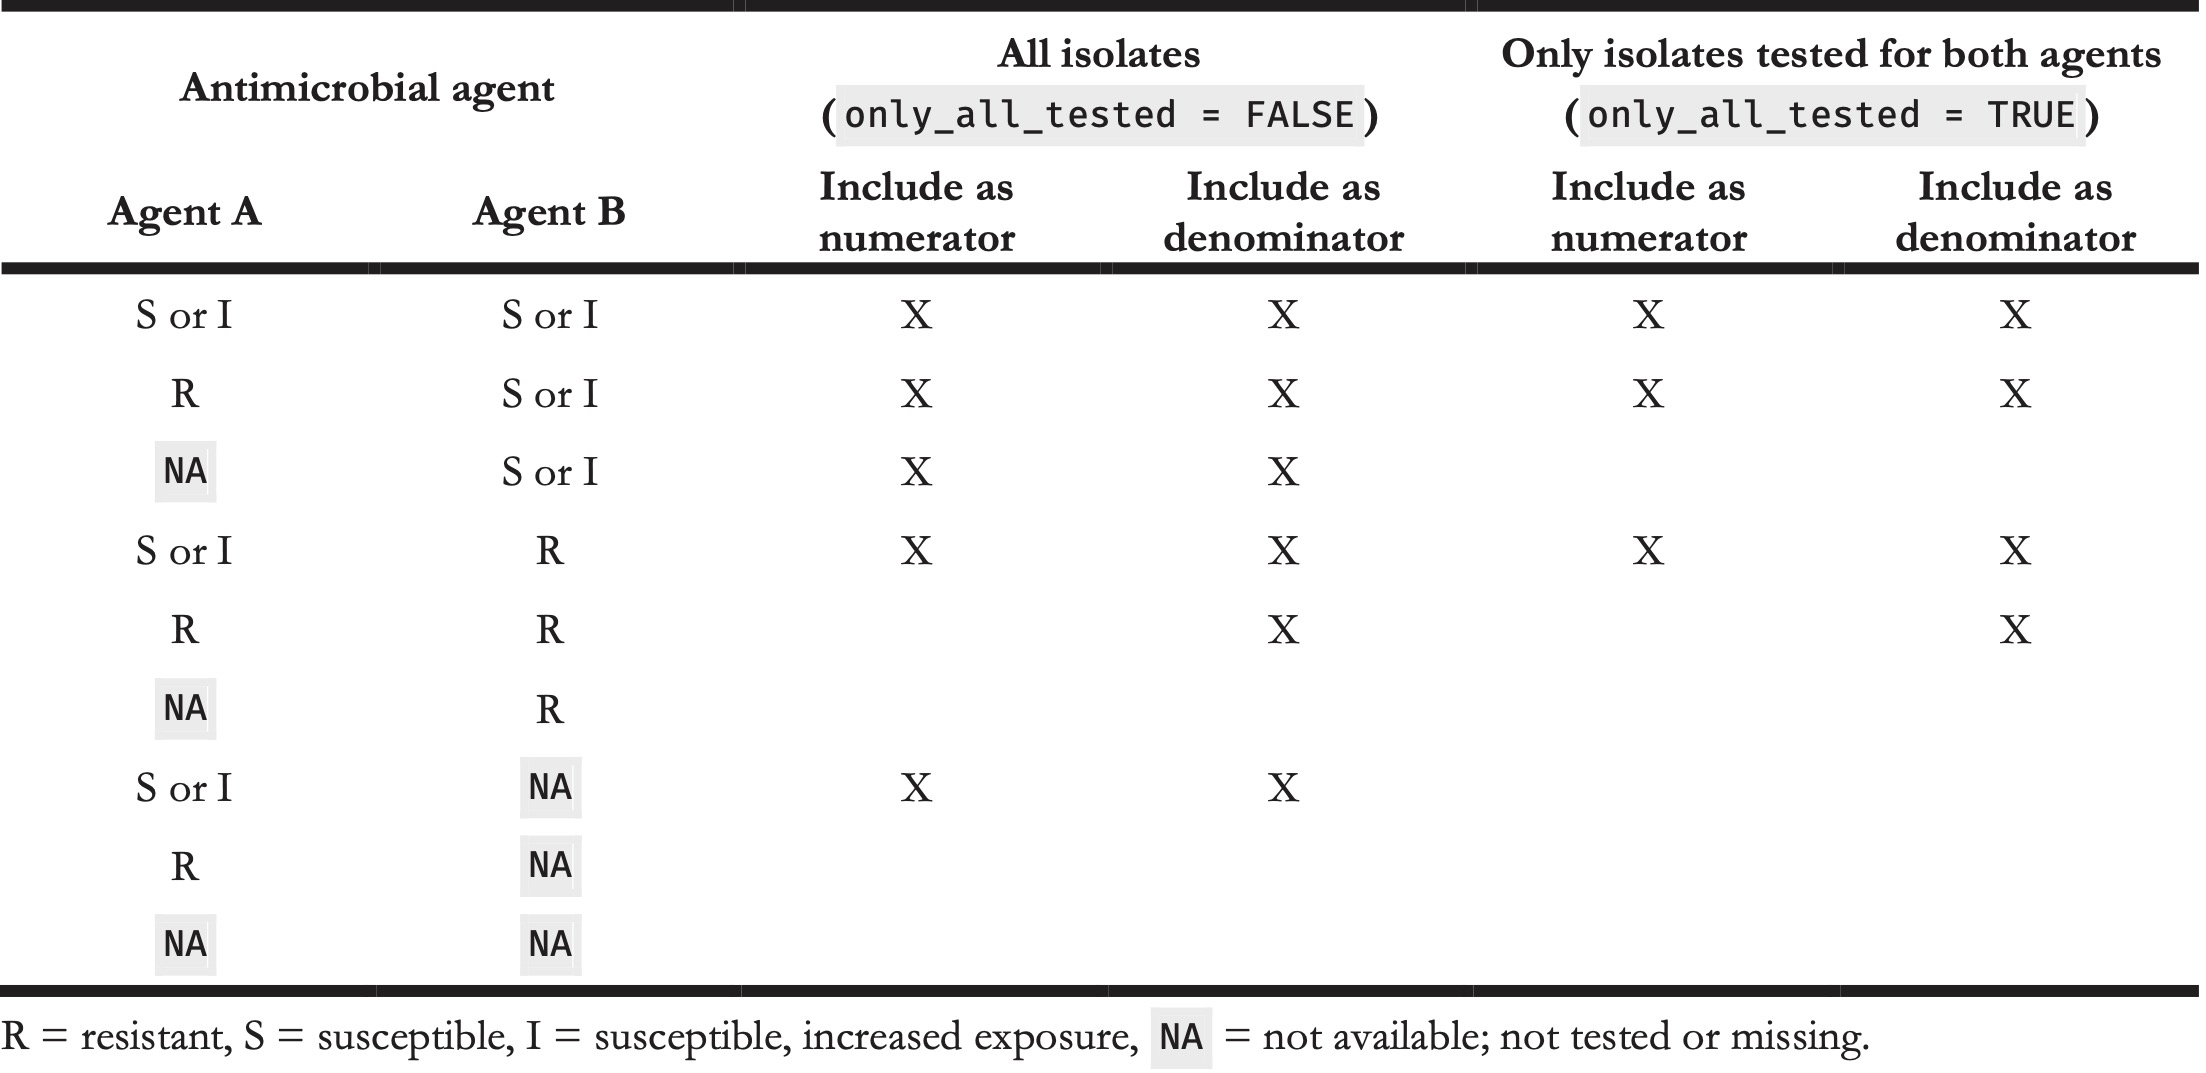
\includegraphics[width=1\linewidth]{images/04-t06} 

}

\end{figure}

The first method is to count the total number of first isolates where at least one agent was tested as ``S'' or ``I'' and divide it by the number of first isolates tested where any of the agents was tested (Equation 4). This method will be used when setting \texttt{only\_all\_tested\ =\ FALSE} in the \texttt{susceptibility()} function:

\[s_{(x, y)} = \frac{\sum_{i=1}^k [x_i \in \{S,I\} \lor y_i \in \{S,I\}]}{\sum_{i=1}^k [x_i \in \{R,S,I\} \lor y_i \in \{R,S,I\}]}\]

where \(x\) is a character vector only consisting of values ``R'', ``S'', or ``I'' (i.e., '\texttt{agent\ A’}) and \(y\) is another character vector only consisting of values ``R'', ``S'', or ``I'' (i.e., '\texttt{agent\ B’}).

The second method is to count the total number of first isolates where at least one agent was tested as ``S'' or ``I'' and where all agents were tested divided by the number of first isolates tested where all of the agents were tested (Equation 5). This method will be used when setting \texttt{only\_all\_tested\ =\ TRUE} in the \texttt{susceptibility()} function:

\[s'_{(x, y)} = \frac{\sum_{i=1}^k [(x_i \in \{S,I\} \lor y_i \in \{S,I\}) \, \land x_i \in \{R,S,I\} \land y_i \in \{R,S,I\}]}{\sum_{i=1}^k [x_i \in \{R,S,I\} \land y_i \in \{R,S,I\}]}\]

Based on Equation 2, the overall resistance and susceptibility of antimicrobial agents like gentamicin (GEN) and amoxicillin (AMX) can be calculated using the following syntax. The \texttt{example\_isolates} data set is an example data set included in the \texttt{AMR} package, see Appendix A. The \texttt{n\_rsi()} function is analogous to the \texttt{n()} function of the \texttt{dplyr} package. It counts the number of available isolates, but only includes observations with valid antimicrobial results (i.e., ``R'', ``S'', or ``I''):

\begin{Shaded}
\begin{Highlighting}[]
\FunctionTok{library}\NormalTok{(}\StringTok{"dplyr"}\NormalTok{)}
\NormalTok{example\_isolates }\SpecialCharTok{\%\textgreater{}\%}
   \FunctionTok{summarise}\NormalTok{(}\AttributeTok{r\_gen =} \FunctionTok{proportion\_R}\NormalTok{(GEN),}
             \AttributeTok{r\_amx =} \FunctionTok{proportion\_R}\NormalTok{(AMX),}
             \AttributeTok{n\_gen =} \FunctionTok{n\_rsi}\NormalTok{(GEN),}
             \AttributeTok{n\_amx =} \FunctionTok{n\_rsi}\NormalTok{(AMX),}
             \AttributeTok{n\_total =} \FunctionTok{n}\NormalTok{())}
\CommentTok{\#\textgreater{}         r\_gen     r\_amx n\_gen n\_amx n\_total}
\CommentTok{\#\textgreater{} [1] 0.2458221 0.5955556  1855  1350    2000}
\end{Highlighting}
\end{Shaded}

This output reads: the resistance to gentamicin of all isolates in the \texttt{example\_isolates} data set is \(P{(x = GEN, o = \{R\})} = 24.6\%\), based on \(1855\) out of \(2000\) available isolates. This means that the susceptibility is \(P{(x = GEN, o = \{S,I\})} = 75.4\%\). The susceptibility to amoxicillin is \(P{(x = AMX, o = \{S,I\})} = 40.4\%\) based on \(1350\) isolates.

To calculate the effect of combination therapy, i.e., treating patients with multiple agents at the same time, all \texttt{proportion\_*()} functions can handle multiple variables as arguments as defined in Equation 4 and 5. For example, to calculate the empiric susceptibility of a combination therapy comprising gentamicin (GEN) and amoxicillin (AMX):

\begin{Shaded}
\begin{Highlighting}[]
\NormalTok{example\_isolates }\SpecialCharTok{\%\textgreater{}\%}
  \FunctionTok{summarise}\NormalTok{(}\AttributeTok{si\_gen\_amx =} \FunctionTok{proportion\_SI}\NormalTok{(GEN, AMX),}
            \AttributeTok{n\_gen\_amx =} \FunctionTok{n\_rsi}\NormalTok{(GEN, AMX),}
            \AttributeTok{n\_total =} \FunctionTok{n}\NormalTok{())}
\CommentTok{\#\textgreater{}     si\_gen\_amx n\_gen\_amx n\_total}
\CommentTok{\#\textgreater{} [1]   0.931843      1921    2000}
\end{Highlighting}
\end{Shaded}

This leads to the conclusion that combining gentamicin with amoxicillin would cover \(s{(x = GEN, y = AMX)} = 93.2\%\) based on \(1921\) out of \(2000\) available isolates, which is \(17.8\%\) more than when treating with gentamicin alone (\(P{(x = GEN, o = \{S,I\})} = 75.4\%\)). With these functions, exact calculations can be done to evaluate the empiric success of treating infections with one or more antimicrobial agents.

\hypertarget{design-decisions}{%
\section{Design decisions}\label{design-decisions}}

The \texttt{AMR} package follows the rationale of tidyverse packages as authored by Wickham \emph{et al.} \textsuperscript{{[}40{]}}. Most functions take a \texttt{‘data.frame’} or \texttt{‘tibble’} as input, support piping (\%\textgreater\%) operations, can work with quasi-quotations, and can be integrated into \texttt{dplyr} workflows, such as \texttt{mutate()} to create new variables and \texttt{group\_by()} to group by variables. Although the \texttt{AMR} package integrates well into tidyverse workflows, it can also be used with base \texttt{R}only. To this extent, the \texttt{AMR} package was developed to be independent of any other \texttt{R}package to ensure and maintain sustainability.

The \texttt{AMR} package supports multiple languages. Currently supported languages are English, Dutch, French, German, Italian, Portuguese, and Spanish. The system language will be used if the language is supported but can be overwritten with \texttt{options(AMR\_locale\ =\ ...)}. Multi-language support affects language-dependent output of functions such as \texttt{mo\_name()}, \texttt{mo\_gramstain()}, \texttt{mo\_type()}, and \texttt{ab\_name()}.

The \texttt{AMR} package uses S3 classes, object oriented (OO) systems available in R. They allow different types of output based on the user input. The \texttt{AMR} package introduces 5 S3 classes (\texttt{‘mo’}, \texttt{‘ab’}, \texttt{‘rsi’}, \texttt{‘mic’}, and \texttt{‘disk’}) to increase the convenience when working with antimicrobial susceptibility data.

\hypertarget{reproducible-example}{%
\section{Reproducible example}\label{reproducible-example}}

We consider the problem of working with antimicrobial resistance data from three different hospitals between 2011-01-01 and 2020-01-01. After loading the \texttt{AMR} package and additional tidyverse packages to allow transformation and plotting, we load the \texttt{example\_isolates}\_unclean example data from the \texttt{AMR} package into the global environment and assign it a new name.

\begin{Shaded}
\begin{Highlighting}[]
\FunctionTok{library}\NormalTok{(}\StringTok{"dplyr"}\NormalTok{)}
\FunctionTok{library}\NormalTok{(}\StringTok{"tidyr"}\NormalTok{)}
\FunctionTok{library}\NormalTok{(}\StringTok{"AMR"}\NormalTok{)}

\FunctionTok{options}\NormalTok{(}\AttributeTok{AMR\_locale =} \StringTok{"en"}\NormalTok{)}

\NormalTok{data }\OtherTok{\textless{}{-}}\NormalTok{ example\_isolates\_unclean}

\FunctionTok{glimpse}\NormalTok{(data)}
\CommentTok{\#\textgreater{} Rows: 3,000}
\CommentTok{\#\textgreater{} Columns: 8}
\CommentTok{\#\textgreater{} $ patient\_id \textless{}chr\textgreater{} "J3", "R7", "P3", "P10", "B7", "W3", "J8", "M3",…}
\CommentTok{\#\textgreater{} $ hospital   \textless{}chr\textgreater{} "A", "A", "A", "A", "A", "A", "A", "A", "A", "A"…}
\CommentTok{\#\textgreater{} $ date       \textless{}date\textgreater{} 2012{-}11{-}21, 2018{-}04{-}03, 2014{-}09{-}19, 2015{-}12{-}10,…}
\CommentTok{\#\textgreater{} $ bacteria   \textless{}chr\textgreater{} "E. coli", "K. pneumoniae", "E. coli", "E. coli"…}
\CommentTok{\#\textgreater{} $ AMX        \textless{}chr\textgreater{} "R", "R", "R", "S", "S", "R", "R", "R", "S", "S"…}
\CommentTok{\#\textgreater{} $ AMC        \textless{}chr\textgreater{} "I", "I", "S", "I", "S", "S", "S", "S", "S", "S"…}
\CommentTok{\#\textgreater{} $ CIP        \textless{}chr\textgreater{} "S", "S", "S", "S", "S", "R", "S", "S", "S", "S"…}
\CommentTok{\#\textgreater{} $ GEN        \textless{}chr\textgreater{} "S", "S", "S", "S", "S", "S", "S", "S", "S", "S"…}

\FunctionTok{unique}\NormalTok{(data}\SpecialCharTok{$}\NormalTok{hospital)}
\CommentTok{\#\textgreater{} [1] "A" "B" "C"}

\FunctionTok{unique}\NormalTok{(data}\SpecialCharTok{$}\NormalTok{bacteria)}
\CommentTok{\#\textgreater{}  [1] "E. coli"                  "K. pneumoniae"           }
\CommentTok{\#\textgreater{}  [3] "S. aureus"                "S. pneumoniae"           }
\CommentTok{\#\textgreater{}  [5] "klepne"                   "strpne"                  }
\CommentTok{\#\textgreater{}  [7] "esccol"                   "staaur"                  }
\CommentTok{\#\textgreater{}  [9] "Escherichia coli"         "Staphylococcus aureus"   }
\CommentTok{\#\textgreater{} [11] "Streptococcus pneumoniae" "Klebsiella pneumoniae"    }

\NormalTok{data }\SpecialCharTok{\%\textgreater{}\%}
  \FunctionTok{count}\NormalTok{(bacteria)}
\CommentTok{\#\textgreater{}                    bacteria   n}
\CommentTok{\#\textgreater{} 1                   E. coli 494}
\CommentTok{\#\textgreater{} 2                    esccol 508}
\CommentTok{\#\textgreater{} 3          Escherichia coli 516}
\CommentTok{\#\textgreater{} 4             K. pneumoniae 108}
\CommentTok{\#\textgreater{} 5     Klebsiella pneumoniae 102}
\CommentTok{\#\textgreater{} 6                    klepne 116}
\CommentTok{\#\textgreater{} 7                 S. aureus 247}
\CommentTok{\#\textgreater{} 8             S. pneumoniae 151}
\CommentTok{\#\textgreater{} 9                    staaur 240}
\CommentTok{\#\textgreater{} 10    Staphylococcus aureus 243}
\CommentTok{\#\textgreater{} 11 Streptococcus pneumoniae 139}
\CommentTok{\#\textgreater{} 12                   strpne 136}
\end{Highlighting}
\end{Shaded}

The data contains 3,000 observations of 8 variables from 3 hospitals. The ``bacteria'' variable comprises 12 unique elements. However, they appear to encode the same information in different formats ('\texttt{E.\ coli’}, '\texttt{K.\ pneumoniae’}, '\texttt{S.\ aureus’}, '\texttt{S.\ pneumoniae’}, '\texttt{klepne’}, '\texttt{strpne’}, '\texttt{esccol’}, '\texttt{staaur’}, '\texttt{Escherichia\ coli’}, '\texttt{Staphylococcus\ aureus’}, '\texttt{Streptococcus\ pneumoniae’}, '\texttt{Klebsiella\ pneumoniae’}). We can use the \texttt{as.mo()} function to standardise the bacterial codes and add a variable with the official scientific name. The correct transformation of the bacterial codes can be reviewed by calling the \texttt{mo\_uncertainties()} function.

\begin{Shaded}
\begin{Highlighting}[]
\NormalTok{data }\OtherTok{\textless{}{-}}\NormalTok{ data }\SpecialCharTok{\%\textgreater{}\%}
  \FunctionTok{mutate}\NormalTok{(}\AttributeTok{bacteria =} \FunctionTok{as.mo}\NormalTok{(bacteria),}
         \AttributeTok{bacteria\_name =} \FunctionTok{mo\_name}\NormalTok{(bacteria))}

\FunctionTok{mo\_uncertainties}\NormalTok{()}
\CommentTok{\#\textgreater{} "E. coli" {-}\textgreater{} Escherichia coli (B\_ESCHR\_COLI, matching score =}
\CommentTok{\#\textgreater{}              0.688)}
\CommentTok{\#\textgreater{}              Also matched: Entamoeba coli (0.079)}
\CommentTok{\#\textgreater{} "K. pneumoniae" {-}\textgreater{} Klebsiella pneumoniae (B\_KLBSL\_PNMN, matching}
\CommentTok{\#\textgreater{}                    score = 0.786)}
\CommentTok{\#\textgreater{}                    Also matched: Klebsiella pneumoniae ozaenae}
\CommentTok{\#\textgreater{}                    (0.707), Klebsiella pneumoniae rhinoscleromatis}
\CommentTok{\#\textgreater{}                    (0.658)}
\CommentTok{\#\textgreater{} }
\CommentTok{\#\textgreater{} "S. aureus" {-}\textgreater{} Staphylococcus aureus (B\_STPHY\_AURS, matching score}
\CommentTok{\#\textgreater{}                = 0.690)}
\CommentTok{\#\textgreater{}                Also matched: Staphylococcus aureus anaerobius}
\CommentTok{\#\textgreater{}                (0.625), Streptomyces aureus (0.355), Stentor aureus}
\CommentTok{\#\textgreater{}                (0.052)}

\NormalTok{data }\SpecialCharTok{\%\textgreater{}\%}
  \FunctionTok{count}\NormalTok{(bacteria, bacteria\_name)}
\CommentTok{\#\textgreater{}       bacteria            bacteria\_name    n}
\CommentTok{\#\textgreater{} 1 B\_ESCHR\_COLI         Escherichia coli 1518}
\CommentTok{\#\textgreater{} 2 B\_KLBSL\_PNMN    Klebsiella pneumoniae  326}
\CommentTok{\#\textgreater{} 3 B\_STPHY\_AURS    Staphylococcus aureus  730}
\CommentTok{\#\textgreater{} 4 B\_STRPT\_PNMN Streptococcus pneumoniae  426}
\end{Highlighting}
\end{Shaded}

In a next step, we can further enrich the data with additional microbial taxonomic data based on the ``bacteria'' variable, such as Gram-stain and microorganism family.

\begin{Shaded}
\begin{Highlighting}[]
\NormalTok{data }\OtherTok{\textless{}{-}}\NormalTok{ data }\SpecialCharTok{\%\textgreater{}\%}
  \FunctionTok{mutate}\NormalTok{(}\AttributeTok{gram\_stain =} \FunctionTok{mo\_gramstain}\NormalTok{(bacteria),}
         \AttributeTok{family =} \FunctionTok{mo\_family}\NormalTok{(bacteria))}

\NormalTok{data }\SpecialCharTok{\%\textgreater{}\%}
  \FunctionTok{count}\NormalTok{(gram\_stain)}
\CommentTok{\#\textgreater{}      gram\_stain    n}
\CommentTok{\#\textgreater{} 1 Gram{-}negative 1844}
\CommentTok{\#\textgreater{} 2 Gram{-}positive 1156}

\NormalTok{data }\SpecialCharTok{\%\textgreater{}\%}
  \FunctionTok{count}\NormalTok{(family)}
\CommentTok{\#\textgreater{}               family    n}
\CommentTok{\#\textgreater{} 1 Enterobacteriaceae 1844}
\CommentTok{\#\textgreater{} 2 Staphylococcaceae   730}
\CommentTok{\#\textgreater{} 3 Streptococcaceae    426}
\end{Highlighting}
\end{Shaded}

The variables ``AMX'', ``AMC'', ``CIP'', and ``GEN'' contain antimicrobial susceptibility test results. The abbreviations stand for the tested antimicrobial agent. The official names and additional information about the antimicrobial agents can be checked with the \texttt{ab\_info()} function from the \texttt{AMR} package.

\begin{Shaded}
\begin{Highlighting}[]
\FunctionTok{ab\_info}\NormalTok{(}\StringTok{"AMX"}\NormalTok{)}
\CommentTok{\#\textgreater{} $ab}
\CommentTok{\#\textgreater{} [1] "AMX"}
\CommentTok{\#\textgreater{} }
\CommentTok{\#\textgreater{} $atc}
\CommentTok{\#\textgreater{} [1] "J01CA04"}
\CommentTok{\#\textgreater{} }
\CommentTok{\#\textgreater{} $cid}
\CommentTok{\#\textgreater{} [1] 33613}
\CommentTok{\#\textgreater{} }
\CommentTok{\#\textgreater{} $name}
\CommentTok{\#\textgreater{} [1] "Amoxicillin"}
\CommentTok{\#\textgreater{} }
\CommentTok{\#\textgreater{} $group}
\CommentTok{\#\textgreater{} [1] "Beta{-}lactams/penicillins"}
\CommentTok{\#\textgreater{} }
\CommentTok{\#\textgreater{} $atc\_group1}
\CommentTok{\#\textgreater{} [1] "Beta{-}lactam antibacterials, penicillins"}
\CommentTok{\#\textgreater{} }
\CommentTok{\#\textgreater{} $atc\_group2}
\CommentTok{\#\textgreater{} [1] "Penicillins with extended spectrum"}
\CommentTok{\#\textgreater{} }
\CommentTok{\#\textgreater{} $tradenames}
\CommentTok{\#\textgreater{} [1] "actimoxi" "amoclen" "amolin" }
\CommentTok{\#\textgreater{} [4] "amopen" "amopenixin" "amoxibiotic" }
\CommentTok{\#\textgreater{} [7] "amoxicaps" "amoxicilina" "amoxicillin" }
\CommentTok{\#\textgreater{} [10] "amoxicilline" "amoxicillinum" "amoxiden" }
\CommentTok{\#\textgreater{} [13] "amoxil" "amoxivet" "amoxy" }
\CommentTok{\#\textgreater{} [16] "amoxycillin" "anemolin" "aspenil" }
\CommentTok{\#\textgreater{} [19] "biomox" "bristamox" "cemoxin" }
\CommentTok{\#\textgreater{} [22] "clamoxyl" "delacillin" "dispermox" }
\CommentTok{\#\textgreater{} [25] "efpenix" "flemoxin" "hiconcil" }
\CommentTok{\#\textgreater{} [28] "histocillin" "hydroxyampicillin" "ibiamox" }
\CommentTok{\#\textgreater{} [31] "imacillin" "lamoxy" "metafarma capsules"}
\CommentTok{\#\textgreater{} [34] "metifarma capsules" "moxacin" "moxatag" }
\CommentTok{\#\textgreater{} [37] "ospamox" "pamoxicillin" "piramox" }
\CommentTok{\#\textgreater{} [40] "robamox" "sawamox pm" "tolodina" }
\CommentTok{\#\textgreater{} [43] "unicillin" "utimox" "vetramox" }
\CommentTok{\#\textgreater{} }
\CommentTok{\#\textgreater{} $ddd}
\CommentTok{\#\textgreater{} $ddd$oral}
\CommentTok{\#\textgreater{} $ddd$oral$amount}
\CommentTok{\#\textgreater{} [1] 1.5}
\CommentTok{\#\textgreater{} }
\CommentTok{\#\textgreater{} $ddd$oral$units}
\CommentTok{\#\textgreater{} [1] "g"}
\CommentTok{\#\textgreater{} }
\CommentTok{\#\textgreater{} }
\CommentTok{\#\textgreater{} $ddd$iv}
\CommentTok{\#\textgreater{} $ddd$iv$amount}
\CommentTok{\#\textgreater{} [1] 3}
\CommentTok{\#\textgreater{} }
\CommentTok{\#\textgreater{} $ddd$iv$units}
\CommentTok{\#\textgreater{} [1] "g"}
\end{Highlighting}
\end{Shaded}

In a data set containing antimicrobial names or codes (e.g., antimicrobial prescription data), the \texttt{as.ab()} function can be used to transform all values to valid antimicrobial codes. Extra columns with the official name and the defined daily dose (DDD) for intravenous administration could be added using \texttt{ab\_name()} and \texttt{ab\_ddd()}.

\begin{Shaded}
\begin{Highlighting}[]
\NormalTok{antimicrobial\_example }\OtherTok{\textless{}{-}} \FunctionTok{data.frame}\NormalTok{(}\AttributeTok{agents =} \FunctionTok{c}\NormalTok{(}\StringTok{"AMX"}\NormalTok{,}
                                               \StringTok{"Ceftriaxon"}\NormalTok{,}
                                               \StringTok{"Cipro"}\NormalTok{))}

\NormalTok{antimicrobial\_example }\SpecialCharTok{\%\textgreater{}\%} 
  \FunctionTok{mutate}\NormalTok{(}\AttributeTok{agents =} \FunctionTok{as.ab}\NormalTok{(agents), }
         \AttributeTok{agent\_names =} \FunctionTok{ab\_name}\NormalTok{(agents),}
         \AttributeTok{ddd\_iv =} \FunctionTok{ab\_ddd}\NormalTok{(agents, }\AttributeTok{administration =} \StringTok{"iv"}\NormalTok{))}
\CommentTok{\#\textgreater{} agents agent\_names ddd\_iv}
\CommentTok{\#\textgreater{} 1 AMX Amoxicillin 3.0}
\CommentTok{\#\textgreater{} 2 CRO Ceftriaxone 2.0}
\CommentTok{\#\textgreater{} 3 CIP Ciprofloxacin 0.8}
\end{Highlighting}
\end{Shaded}

Coming back to the cleaning of the data, the columns for the antimicrobial susceptibility test results (``AMX'', ``AMC'', ``CIP'', ``GEN'') need to be checked to contain only standard values (``R'', ``S'', ``I'').

\begin{Shaded}
\begin{Highlighting}[]
\NormalTok{data }\SpecialCharTok{\%\textgreater{}\%}
  \FunctionTok{select}\NormalTok{(AMX}\SpecialCharTok{:}\NormalTok{GEN) }\SpecialCharTok{\%\textgreater{}\%}
  \FunctionTok{pivot\_longer}\NormalTok{(}\FunctionTok{everything}\NormalTok{(),}
               \AttributeTok{names\_to =} \StringTok{"antimicrobials"}\NormalTok{,}
               \AttributeTok{values\_to =} \StringTok{"interpretation"}\NormalTok{) }\SpecialCharTok{\%\textgreater{}\%}
  \FunctionTok{count}\NormalTok{(interpretation)}
\CommentTok{\#\textgreater{} \# A tibble: 4 x 2}
\CommentTok{\#\textgreater{}   interpretation     n}
\CommentTok{\#\textgreater{}   \textless{}chr\textgreater{}          \textless{}int\textgreater{}}
\CommentTok{\#\textgreater{} 1 \textless{} 0.5 S          143}
\CommentTok{\#\textgreater{} 2 I               1105}
\CommentTok{\#\textgreater{} 3 R               4607}
\CommentTok{\#\textgreater{} 4 S               6145}
\end{Highlighting}
\end{Shaded}

The values contain some mixed values. The \texttt{as.rsi()} function can be used to clean these values and to assign a new class (\texttt{‘rsi’}) for further use of AMR functions.

\begin{Shaded}
\begin{Highlighting}[]
\NormalTok{data }\OtherTok{\textless{}{-}}\NormalTok{ data }\SpecialCharTok{\%\textgreater{}\%}
  \FunctionTok{mutate\_at}\NormalTok{(}\FunctionTok{vars}\NormalTok{(AMX}\SpecialCharTok{:}\NormalTok{GEN), as.rsi)}

\NormalTok{data }\SpecialCharTok{\%\textgreater{}\%}
  \FunctionTok{select}\NormalTok{(AMX}\SpecialCharTok{:}\NormalTok{GEN) }\SpecialCharTok{\%\textgreater{}\%}
  \FunctionTok{pivot\_longer}\NormalTok{(}\FunctionTok{everything}\NormalTok{(),}
               \AttributeTok{names\_to =} \StringTok{"antimicrobials"}\NormalTok{,}
               \AttributeTok{values\_to =} \StringTok{"interpretation"}\NormalTok{) }\SpecialCharTok{\%\textgreater{}\%}
  \FunctionTok{count}\NormalTok{(interpretation)}
\CommentTok{\#\textgreater{} \# A tibble: 3 x 2}
\CommentTok{\#\textgreater{}   interpretation     n}
\CommentTok{\#\textgreater{}   \textless{}rsi\textgreater{}          \textless{}int\textgreater{}}
\CommentTok{\#\textgreater{} 1   S             6288}
\CommentTok{\#\textgreater{} 2   I             1105}
\CommentTok{\#\textgreater{} 3   R             4607}
\end{Highlighting}
\end{Shaded}

After this transformation, the \texttt{eucast\_rules()} function can be applied to apply the latest resistance reporting guidelines.

\begin{Shaded}
\begin{Highlighting}[]
\NormalTok{data }\OtherTok{\textless{}{-}}\NormalTok{ data }\SpecialCharTok{\%\textgreater{}\%}
  \FunctionTok{eucast\_rules}\NormalTok{()}
\end{Highlighting}
\end{Shaded}

The output to the console lists the changes made to data:

\begin{Shaded}
\begin{Highlighting}[]
\CommentTok{\#\textgreater{} The rules affected 508 out of 3,000 rows, making a total of 657 edits}
\CommentTok{\#\textgreater{} =\textgreater{} added 0 test results}
\CommentTok{\#\textgreater{} }
\CommentTok{\#\textgreater{} =\textgreater{} changed 657 test results}
\CommentTok{\#\textgreater{} {-} 11 test results changed from "S" to "I"}
\CommentTok{\#\textgreater{} {-} 473 test results changed from "S" to "R"}
\CommentTok{\#\textgreater{} {-} 85 test results changed from "I" to "R"}
\CommentTok{\#\textgreater{} {-} 19 test results changed from "I" to "S"}
\CommentTok{\#\textgreater{} {-} 33 test results changed from "R" to "I"}
\CommentTok{\#\textgreater{} {-} 36 test results changed from "R" to "S"}
\end{Highlighting}
\end{Shaded}

The data is now clean and ready for further analysis, for example, the identification of multi-drug resistant microorganisms. In this example, we use the Dutch guideline to determine multi-drug resistance \textsuperscript{{[}35{]}}.

\begin{Shaded}
\begin{Highlighting}[]
\NormalTok{data }\OtherTok{\textless{}{-}}\NormalTok{ data }\SpecialCharTok{\%\textgreater{}\%}
  \FunctionTok{mutate}\NormalTok{(}\AttributeTok{mdro =} \FunctionTok{mdro}\NormalTok{(., }\AttributeTok{guideline =} \StringTok{"nl"}\NormalTok{))}

\NormalTok{data }\SpecialCharTok{\%\textgreater{}\%}
  \FunctionTok{count}\NormalTok{(bacteria\_name, mdro)}
\CommentTok{\#\textgreater{}              bacteria\_name     mdro    n}
\CommentTok{\#\textgreater{} 1         Escherichia coli Negative 1123}
\CommentTok{\#\textgreater{} 2         Escherichia coli Positive  395}
\CommentTok{\#\textgreater{} 3    Klebsiella pneumoniae Negative  237}
\CommentTok{\#\textgreater{} 4    Klebsiella pneumoniae Positive   89}
\CommentTok{\#\textgreater{} 5    Staphylococcus aureus Negative  730}
\CommentTok{\#\textgreater{} 6 Streptococcus pneumoniae Negative  426}
\end{Highlighting}
\end{Shaded}

According to the Dutch guideline, 484 (395 + 89) multi-drug resistant microorganisms were found in 3,000 tested isolates. No multi-drug resistance was found in Staphylococcus aureus and Streptococcus pneumoniae.

As described in Section 4.4.1, the identification of first isolates is essential for the reporting of resistance patterns. Using the \texttt{filter\_first\_isolate()} function and \texttt{proportion\_df()} in combination with \texttt{group\_by()}, we get a complete resistance analysis per hospital, bacteria, first isolate, and tested antimicrobial agent in one call:

\begin{Shaded}
\begin{Highlighting}[]
\NormalTok{resistance\_proportion }\OtherTok{\textless{}{-}}\NormalTok{ data }\SpecialCharTok{\%\textgreater{}\%}
  \FunctionTok{filter\_first\_isolate}\NormalTok{() }\SpecialCharTok{\%\textgreater{}\%}
  \FunctionTok{group\_by}\NormalTok{(hospital) }\SpecialCharTok{\%\textgreater{}\%}
  \FunctionTok{proportion\_df}\NormalTok{()}

\FunctionTok{head}\NormalTok{(resistance\_proportion)}
\CommentTok{\#\textgreater{}   hospital                  antibiotic interpretation     value}
\CommentTok{\#\textgreater{} 1        A                 Amoxicillin             SI 0.5773050}
\CommentTok{\#\textgreater{} 2        A                 Amoxicillin              R 0.4226950}
\CommentTok{\#\textgreater{} 3        A Amoxicillin/clavulanic acid             SI 0.8085106}
\CommentTok{\#\textgreater{} 4        A Amoxicillin/clavulanic acid              R 0.1914894}
\CommentTok{\#\textgreater{} 5        A               Ciprofloxacin             SI 0.8042553}
\CommentTok{\#\textgreater{} 6        A               Ciprofloxacin              R 0.1957447}
\end{Highlighting}
\end{Shaded}

From the console we get the information how many first isolates were identified and used in the filter.

From here on, the data is ready for further analysis with functions for plotting (e.g., the \texttt{ggplot2} package \textsuperscript{{[}41{]}}), AMR extension functions for base \texttt{R}(e.g., \texttt{summary()}, \texttt{plot()}), or \texttt{AMR} helper functions for plotting and basic modelling (e.g., \texttt{ggplot\_rsi()}, \texttt{geom\_rsi()}, \texttt{resistance\_predict()}).

\hypertarget{discussion}{%
\section{Discussion}\label{discussion}}

For the first time, a free and open-source software solution is available to cover all aspects of working with antimicrobial resistance data. The \texttt{AMR} package provides functionalities that enable standardised and reproducible workflows from raw laboratory data to publishable results, for research and clinical workflows alike. In the field of clinical microbiology and infectious diseases, research and clinical workflows are closely linked. For example, a performed research study on the prevalence of antimicrobial-resistant bacteria can have direct implications on the choice of antimicrobial agents for the treatment of patients. The \texttt{AMR} package was developed to be used in any research or clinical setting where the data analysis on microorganisms, antimicrobial resistance, antimicrobial agents is required.

Both, researchers and clinicians rely on the data from electronic laboratory information systems (LIS) where laboratory test results are processed, stored, and archived. Although some commercial solutions exist to conduct medical microbiological data analysis, these solutions are not comprehensive enough to apply antimicrobial resistance analysis for any clinical or research setting. Costs of these tools are a further constraint in resource-limited settings. Moreover, researchers and clinicians that require data from multiple LIS sources to be used in multi-center studies experience major barriers which cannot be solved by available commercial solutions.

Firstly, simple codes for microorganisms show substantial differences between different LIS and presumably correct taxonomic names are often misspelled or outdated. We analysed the taxonomic names of bacteria used in reports from seven different public health institutions that perform microbiological diagnostics in the Netherlands and compared them with an official scientific up-to-date source for microbial taxonomy, the Catalogue of Life \textsuperscript{{[}16{]}}. These institutions cover microbiological diagnostics for hospitals and primary care for 15\% of the total Dutch population. All institutions reported outdated taxonomic names with a maximum lag ranging between 34 and 41 years. Given that antimicrobial resistance guidelines are strongly based on the microbial taxonomy (some rules only apply to a specific genus, other rules apply to a specific family), it is crucial that this information is correct and timely updated. All institutions admitted that there was no standard operating procedure to maintain their taxonomic reference data. Implementing and maintaining the taxonomic data for these and other institutions has been challenging, since no common machine-readable, reliable and up-to-date resource for the microbial taxonomy was publicly available. For reliable reference data about antimicrobial agents, this also holds true. The \texttt{AMR} package provides machine-readable reference data files for the complete microbial taxonomy and for more than 500 antimicrobial agents. Using functions starting with \texttt{mo\_*} and \texttt{ab\_*}, names of microorganisms and antimicrobial agents can be translated between different LIS codes or other forms of text codes for microorganisms and consequently allows to merge data sets from different sites with little effort.

Secondly, antimicrobial resistance interpretation guidelines \textsuperscript{{[}5,6{]}} and taxonomic definitions of microorganisms are under constant change and are continually published in dedicated peer-reviewed journals. This is further complicated by differences between local, regional, and national guidelines. Yet, comparability and reproducibility across setting and time are key in research and clinics. The \texttt{AMR} package functions \texttt{eucast\_rules()} (to apply guidelines to data), \texttt{mdro()} (to check for multi-drug resistance according to guidelines), or \texttt{first\_isolate()} (to determine first isolates according to guidelines) address the needs to standardise comparability, and empower data analysts beyond the capabilities of their local LIS. The \texttt{AMR} package can be used as an extra layer of data validation when retrieving raw data from a LIS. Overall, the functionality of the \texttt{AMR} package has the potential to improve data validity in clinical settings, to ease multi-center study workflows, and to foster research reporting practices. The inherent global nature of antimicrobial resistances requires researchers, clinicians, and policy makers to reach beyond the borders of their local laboratory. The \texttt{AMR} package can build the bridge to link these sources and further encourages open science principles through its open-source approach.

The \texttt{AMR} package also has limitations. It does not introduce novel statistical tests or models, nor does it add additional analytical approaches for AMR research. The calculation of the proportion of susceptibility for more than one antimicrobial agent simultaneously (see Section 4.5.1) seems simple but is subject to unclear reporting in clinical practice \textsuperscript{{[}42,43{]}}. The lack of clearly defined algorithms can lead to the effect that co-resistance rates for more than one antimicrobial agent are dropped altogether \textsuperscript{{[}44{]}}. The inclusion of isolates that are tested for some agents (only\_all\_tested = FALSE) or only isolates tested for all agents (only\_all\_tested = TRUE) can have an imminent clinical impact on patient care, if one combination of antimicrobial agents is preferred over another. Therefore, the \texttt{AMR} package provides different algorithms to standardise this crucial calculation. Unfortunately, unambiguous methodology for determining the right algorithm is lacking in scientific literature. An analysis on the algorithms used in the \texttt{AMR} package and their clinical impact is in preparation.

Reliable information about antimicrobial resistance is vital for clinical decision-making in infectious diseases, since the outcome of local antimicrobial resistance analyses support medical professionals/clinicians in the treatment choices for their patients. Moreover, when this information can be reliably stratified by, for example, year, hospital, and type of patients, new information can lead to new insights for choosing the best antimicrobial therapy for patients suffering from infections. The \texttt{AMR} package enables this by providing all required analysis tools and can therefore empower decision-making in infectious management. The \texttt{AMR} package is already being applied to this end in six hospitals in the Netherlands. The choice of empirical antimicrobial treatment (meaning; choosing the initial therapy at a time of not knowing the infection-causing pathogen) for septic non-post-surgical patients has been altered in at least one Dutch hospital, by analysing antimicrobial resistance data with the \texttt{AMR} package. The clinical effect of this adjustment is being studied at the moment. To improve the quality of such analyses, planned future developments comprise the implementations of an imputation algorithm specifically for antimicrobial agents, and method guidance for applying prediction modelling in a health care setting based on patient-specific properties.

Since the first package release, users from different public and private settings have been suggesting additional functionalities, in particular, the incorporation of country- or time- specific guidelines (e.g., Magiorakos \emph{et al.} \textsuperscript{{[}31{]}}). This community-centred development will be continued and maintained by researchers at the University Medical Center Groningen and data scientists at Certe Medical Diagnostics and Advice, both non-profit public health organisations located in Groningen, the Netherlands. Moreover, a group of contributors from five different Dutch health care institutions has been formed at the Dutch Association for Medical Microbiology (Nederlandse Vereniging voor Medische Microbiologie - NVMM) that also peer-review major changes to the package, including the implementation of guideline updates. This way, updates required for scientific developments as well as maintaining consistent reproducibility are ensured. Updates to databases and guidelines included in the \texttt{AMR} package are incorporated on a regular and automated basis, while preserving version control. Any function making use of guidelines (e.g., \texttt{eucast\_rules()}) refers to the latest implemented version of the guideline by default.

The aim of the \texttt{AMR} package is to provide a comprehensive toolbox of solutions for antimicrobial resistance data processing and analysis on an institution- and country-independent scale for clinical practice and research that are required according to international standards, but were not available to date.

\hypertarget{computational-details}{%
\section*{Computational Details}\label{computational-details}}
\addcontentsline{toc}{section}{Computational Details}

The results in this paper were obtained using \texttt{R}4.0.2 in RStudio 1.3.1093 \textsuperscript{{[}45{]}} with the \texttt{AMR} package 1.5.0, running under macOS Catalina 10.15.

\texttt{R}itself and all packages used are available from the Comprehensive \texttt{R}Archive Network (CRAN) at \url{https://CRAN.R-project.org/}. All development versions of the \texttt{AMR} package are available at \url{https://github.com/msberends/AMR/}.

\hypertarget{acknowledgements}{%
\section*{Acknowledgements}\label{acknowledgements}}
\addcontentsline{toc}{section}{Acknowledgements}

The authors Matthijs S. Berends and Christian F. Luz contributed equally to this publication.

For their contributions to the development of the \texttt{AMR} package, we would like to thank (in alphabetical order) Judith M. Fonville, Erwin E.A. Hassing, Eric H.L.C.M. Hazenberg, Gwen Knight, Annick Lenglet, Bart C. Meijer, Sofia Ny, Rogier P. Schade, Dennis Souverein, and Anthony Underwood.

The development of the \texttt{AMR} package was partly supported by the INTERREG V A (202085) funded project EurHealth-1Health (\url{http://www.eurhealth1health.eu}), part of a Dutch-German cross-border network supported by the European Commission, the Dutch Ministry of Health, Welfare and Sport, the Ministry of Economy, Innovation, Digitalisation and Energy of the German Federal State of North Rhine-Westphalia and the Ministry for National and European Affairs and Regional Development of Lower Saxony.

Furthermore, the \texttt{AMR} package was developed as part of a project funded by the European Commission Horizon 2020 Framework Marie Skłodowska-Curie Actions (grant agreement number: 713660-PRONKJEWAIL-H2020-MSCA-COFUND-2015).

The funders had no role in study design, data collection and analysis, decision to publish, or preparation of the manuscript.

\hypertarget{references-3}{%
\section*{References}\label{references-3}}
\addcontentsline{toc}{section}{References}

\begin{enumerate}
\def\labelenumi{\arabic{enumi}.}
\tightlist
\item
  O'Neill J. Review on antimicrobial resistance: tackling a crisis for the health and wealth of nations. London: Wellcome Trust; 2014.
\item
  De Kraker MEA, Stewardson AJ, Harbarth S. Will 10 million people die a year due to antimicrobial resistance by 2050? PLoS Med 2016;13:e1002184.
\item
  Centers for Disease Control and Prevention. AR threats report: antibiotic resistance threats in the United States, 2019. Atlanta: Centers for Disease Control and Prevention; 2019.
\item
  The European Committee on Antimicrobial Susceptibility Testing. New definitions of S, I and R from 2019; 2019. \url{https://www.eucast.org/newsiandr/}.
\item
  Leclercq R, Cantón R, Brown DFJ, Giske CG, Heisig P, MacGowan AP, \emph{et al.} EUCAST Expert Rules In Antimicrobial Susceptibility Testing. Clin Microbiol Infect 2013;19:141--160.
\item
  Clinical and Laboratory Standards Institute. M39-A4, analysis and presentation of cumulative antimicrobial susceptibility test data, 4th edition. Pittsburgh: Clinical and Laboratory Standards Institute; 2014.
\item
  World Health Organization. Global antimicrobial resistance surveillance system (GLASS) report: early implementation 2017-2018. Geneva: World Health Organization; 2018.
\item
  Tacconelli E, Sifakis F, Harbarth S, Schrijver R, van Mourik M, Voss A, \emph{et al.} Surveillance for control of antimicrobial resistance. Lancet Infect Dis 2018;18:e99--e106.
\item
  Limmathurotsakul D, Dunachie S, Fukuda K, Feasey NA, Okeke IN, Holmes AH, \emph{et al.} Improving the estimation of the global burden of antimicrobial resistant infections. Lancet Infect Dis 2019;19:e392--8.
\item
  R Core Team. R: A language and environment for statistical computing. Vienna: R Foundation for Statistical Computing; 2019.
\item
  Berends MS, Luz CF, Friedrich AW, Sinha BNM, Albers CJ, Glasner C. AMR: Antimicrobial resistance analysis. R package version 1.5.0; 2020. \url{https://CRAN}. R-project.org/package=AMR.
\item
  Lowndes JSS, Best BD, Scarborough C, Afflerbach JC, Frazier MR, O'Hara CC, \emph{et al.} Our path to better science in less time using open data science tools. Nat Ecol Evol 2017;1:160.
\item
  Jombart T, Kamvar ZN, FitzJohn R, Cai J, Bhatia S, Schumacher J, \emph{et al.} incidence: compute, handle, plot and model incidence of dated events. R package version 1.7.3; 2020. \url{https://doi.org/10.5281/zenodo.2584018}.
\item
  Nagraj V, Jombart T, Randhawa N, Sudre B, Campbell F, Crellen T. epicontacts: handling, visualisation and analysis of epidemiological contacts. R package version 1.1.0 2017. \url{https://CRAN.R-project.org/package=epicontacts}.
\item
  Petzoldt T. antbioticR: Analysis of Antibiotic Resistance Data. R package version 0.3.2; 2019. \url{https://github.com/tpetzoldt/antibioticR}.
\item
  Roskov Y, Ower G, Orrell T, Nicolson D, Bailly N, Kirk PM, \emph{et al.} Species 2000 \& ITIS catalogue of life; 2019. www.catalogueoflife.org/col.
\item
  Levenshtein VI.Binary codes capable of correcting deletions, insertions, and reversals. Soviet physics doklady 1966;10:707--710.
\item
  De Greeff SC, Mouton JW, Schoffelen AF, Verduin CM (2019). ``NethMap 2019: consumption of antimicrobial agents and antimicrobial resistance among medically important bacteria in the Netherlands in 2019/ MARAN 2019: monitoring of antimicrobial resistance and antibiotic usage in animals in the Netherlands in 2019. Bilthoven: Rijksinstituut voor Volksgezondheid en Milieu; 2020.
\item
  European Centre for Disease Prevention and Control. European antimicrobial resistance surveillance network (EARS-Net); 2010. \url{https://ecdc.europa.eu/en/about-us/partnerships-and-networks/disease-and-laboratory-networks/ears-net}.
\item
  Cavalier-Smith T. The neomuran origin of archaebacteria, the negibacterial root of the universal tree and bacterial megaclassification. Int J Syst Evol Microbiol 2002;52:7--76.
\item
  WHO Collaborating Centre for Drug Statistics Methodology. Guidelines for ATC classification and DDD assignment 2019. Oslo: WHO Collaborating Centre for Drug Statistics Methodology; 2019.
\item
  European Centre for Disease Prevention and Control. Antimicrobial resistance (AMR) reporting protocol 2018. European antimicrobial resistance surveillance network (EARS-Net) surveillance data for 2017. Stockholm: European Centre for Disease Prevention and Control; 2018.
\item
  Kim S, Chen J, Cheng T, Gindulyte A, He J, He S, \emph{et al.} PubChem 2019 update: improved access to chemical data. Nucleic Acids Res 2019;47:D1102--9.
\item
  Clinical and Laboratory Standards Institute. Susceptibility testing of infectious agents and evaluation of performance of antimicrobial susceptibility test devices -- part 1, 2nd edition. Pittsburgh: Clinical and Laboratory Standards Institute; 2019
\item
  The European Committee on Antimicrobial Susceptibility Testing. breakpoint tables for interpretation of mics and zone diameters, version 10.0, 2020; 2020. \url{http://www.eucast.org/clinical_breakpoints/}.
\item
  Winstanley T, Courvalin P. Expert systems in clinical microbiology. Clin Microbiol Rev 2011;24:515--556.
\item
  Courvalin P. Interpretive reading of antimicrobial susceptibility tests. Molecular analysis and therapeutic interpretation of in vitro tests to improve antibiotic therapy. ASM American Society for Microbiology News 1992;58:368--75.
\item
  Courvalin P. Interpretive reading of in vitro antibiotic susceptibility tests (the antibiogramme). Clin Microbiol Infect 1996;2 Suppl 1:S26--34.
\item
  Livermore DM, Winstanley TG, Shannon KP. Interpretative reading: recognizing the unusual and inferring resistance mechanisms from resistance phenotypes. J Antimicrob Chemother 2001;48 Suppl 1:87--102.
\item
  WHO Collaborating Center for Drug Statistics Methodology. ATC/DDD index; 2019 \url{https://www.whocc.no/atc_ddd_index/}
\item
  Magiorakos A-P, Srinivasan A, Carey RB, Carmeli Y, Falagas ME, Giske CG, \emph{et al.} Multidrug-resistant, extensively drug-resistant and pandrug-resistant bacteria: an international expert proposal for interim standard definitions for acquired resistance. Clin Microbiol Infect 2012;18:268--81.
\item
  Abat C, Fournier P-E, Jimeno M-T, Rolain J-M, \emph{et al.} Extremely and pandrug-resistant bacteria extra-deaths: myth or reality? Eur J Clin Microbiol Infect Dis 2018;37:1687--97.
\item
  European Committee on Antimicrobial Susceptibility Testing (2016). EUCAST expert rules, intrinsic resistance and exceptional phenotypes tables. Version 3.1, 2016; 2016. \url{http://www.eucast.org/fileadmin/src/media/PDFs/EUCAST_files/} Expert\_Rules/Expert\_rules\_intrinsic\_exceptional\_V3.1.pdf.
\item
  World Health Organization. Companion handbook to the WHO guidelines for the programmatic management of drug-resistant tuberculosis. Geneva: World Health Organization; 2014.
\item
  Werkgroep Infectiepreventie. Bijzonder resistente micro-organismen (BRMO). Leiden: Werkgroep Infectiepreventie; 2011.
\item
  Müller J, Voss A, Köck R, Sinha B, Rossen JW, Kaase M, \emph{et al.} Cross-border comparison of the Dutch and German guidelines on multidrug-resistant Gram-negative microorganisms. Antimicrob Resist Infect Control 2015;4:7.
\item
  World Health Organization. Global Tuberculosis Report 2018. Geneva: World Health Organization; 2018.
\item
  Wickham H. Tidy data. J Stat Softw 2014;59:1--23.
\item
  Wickham H, François R, Henry L, Müller K. dplyr: a grammar of data manipulation. R package version 1.0.2; 2020.
\item
  Wickham H, Averick M, Bryan J, Chang W, McGowan L, François R, \emph{et al.} Welcome to the tidyverse. J Open Source Softw 2019;4:1686.
\item
  Wickham H. ggplot2: elegant graphics for data analysis. New York: Springer; 2009.
\item
  Schechner V, Temkin E, Harbarth S, Carmeli Y, Schwaber MJ. Epidemiological interpretation of studies examining the effect of antibiotic usage on resistance. Clin Microbiol Rev 2013;26:289--307.
\item
  Ma J, Li N, Liu Y, Wang C, Liu X, Chen S, \emph{et al.} Antimicrobial resistance patterns, clinical features, and risk factors for septic shock and death of nosocomial E. coli bacteremia in adult patients with hematological disease. Medicine 2017;96:e6959.
\item
  Baur D, Gladstone BP, Burkert F, Carrara E, Foschi F, Döbele S, \emph{et al.} Effect of antibiotic stewardship on the incidence of infection and colonisation with antibiotic-resistant bacteria and Clostridium difficile infection: a systematic review and meta-analysis. Lancet Infect Dis 2017;17:990--1001.
\item
  RStudio Team. RStudio: integrated development environment for R; 2020. \url{http://www.rstudio.com/}.
\item
  WHO Collaborating Centre for Surveillance of Antimicrobial Resistance. WHONET; 2019. \url{http://www.whonet.org/}
\end{enumerate}

\hypertarget{appendix-a-included-data-sets}{%
\section*{Appendix A: Included Data Sets}\label{appendix-a-included-data-sets}}
\addcontentsline{toc}{section}{Appendix A: Included Data Sets}

\begin{itemize}
\item
  \texttt{microorganisms}

  A \texttt{‘data.frame’} containing 67,151 (sub)species with 16 columns comprising their complete microbial taxonomy according to the Catalogue of Life \textsuperscript{{[}16{]}}. Included microorganisms and their complete taxonomic tree of all included (sub)species from kingdom to subspecies with year of scientific publication and responsible author(s):

  \begin{itemize}
  \tightlist
  \item
    All 55,415 (sub)species from the kingdoms of Archaea, Bacteria, Chromista and Protozoa;
  \item
    All 9,582 (sub)species from these orders of the kingdom of Fungi: Eurotiales, Onygenales, Pneumocystales, Saccharomycetales, Schizosaccharomycetales and Tremellales;
  \item
    All 2,153 (sub)species from 47 other relevant genera from the kingdom of Animalia (like Strongyloides and Taenia);
  \item
    All 12,708 previously accepted names of included (sub)species that have been taxonomically renamed.
  \end{itemize}

  The kingdom of Fungi is a very large taxon with almost 300,000 different (sub)species, of which most are not microbial (but rather macroscopic, such as mushrooms). Therefore, not all fungi fit the scope of the \texttt{AMR} package. By only including the aforementioned taxonomic orders, the most relevant fungi are covered (such as all species of Aspergillus, Candida, Cryptococcus, Histoplasma, Pneumocystis, Saccharomyces and Trichophyton).
\item
  \texttt{antibiotics}

  A \texttt{‘data.frame’} containing 456 antibiotic agents with 14 columns. All entries in this data set have three different identifiers: a human readable EARS-Net code (as used by ECDC \textsuperscript{{[}19{]}} and WHONET \textsuperscript{{[}46{]}} and primarily used by this package), an ATC code (as used by the WHO \textsuperscript{{[}21{]}}), and a CID code (Compound ID, as used by PubChem \textsuperscript{{[}23{]}}). The data set contains more than 5,000 official brand names from many different countries, as found in PubChem. Other properties in this data set are derived from one or more of these codes, such as official names of pharmacological and chemical subgroups, and defined daily doses (DDD).
\item
  \texttt{antivirals}

  A \texttt{‘data.frame’} containing 102 antiviral agents with 9 columns. Like the \texttt{antibiotics} data set, it contains ATC codes (as used by the WHO \textsuperscript{{[}21{]}}), and a CID code (Compound ID, as used by PubChem \textsuperscript{{[}23{]}}), as well as the official name and defined daily dose (DDD) for each antiviral agent.
\item
  \texttt{example\_isolates}

  A \texttt{‘data.frame’} containing test results of 2,000 microbial isolates. The data set reflects real patient data and can be used to practice AMR analysis. It is structured in the typical format of laboratory information systems with one row per isolate and one column per tested antimicrobial agent (i.e., an antibiogram).
\item
  \texttt{example\_isolates\_unclean}

  A \texttt{‘data.frame’} containing test results of 3,000 microbial isolates that require cleaning up before they can be used for analysis. This data set can be used to practice AMR analysis and is featured in section 4.7.
\item
  \texttt{WHONET}

  A `\texttt{‘data.frame’} containing 500 observations and 53 columns, with the exact same structure as an export file from WHONET 2019 software \textsuperscript{{[}46{]}}. Such files can be used with the \texttt{AMR} package, as this example data set demonstrates. The antibiotic test results are from the \texttt{example\_isolates} data set. All patient names are created using online surname generators and are only in place for practice purposes.
\end{itemize}

\hypertarget{ch05-radar}{%
\chapter{Rapid Analysis of Diagnostic and Antimicrobial Patterns in R (RadaR): Interactive Open-Source Software App for Infection Management and Antimicrobial Stewardship}\label{ch05-radar}}

Published in Journal of Medical Internet Research, 2019 (21);6, e12843

Luz CF \textsuperscript{1}, Berends MS \textsuperscript{1,2}, Dik JWH \textsuperscript{1}, Lokate ML \textsuperscript{1}, Pulcini C \textsuperscript{3,4}, Glasner C \textsuperscript{1}, Sinha BNM \textsuperscript{1}

\begin{enumerate}
\def\labelenumi{\arabic{enumi}.}
\tightlist
\item
  University of Groningen, University Medical Center Groningen, Department of Medical Microbiology and Infection Prevention, Groningen, The Netherlands
\item
  Certe Medical Diagnostics and Advice Foundation, Groningen, The Netherlands
\item
  Université de Lorraine, APEMAC, Nancy, France
\item
  Université de Lorraine, CHRU-Nancy, Infectious Diseases Department, Nancy, France
\end{enumerate}

\hypertarget{abstract-3}{%
\section*{Abstract}\label{abstract-3}}
\addcontentsline{toc}{section}{Abstract}

Analysing process and outcome measures for all patients diagnosed with an infection in a hospital, including those suspected of having an infection, requires not only processing of large datasets but also accounting for numerous patient parameters and guidelines. Substantial technical expertise is required to conduct such rapid, reproducible, and adaptable analyses; however, such analyses can yield valuable insights for infection management and antimicrobial stewardship (AMS) teams. The aim of this study was to present the design, development, and testing of RadaR (Rapid analysis of diagnostic and antimicrobial patterns in R), a software app for infection management, and to ascertain whether RadaR can facilitate user-friendly, intuitive, and interactive analyses of large datasets in the absence of prior in-depth software or programming knowledge. RadaR was built in the open-source programming language R, using Shiny, an additional package to implement web-app frameworks in R. It was developed in the context of a 1339-bed academic tertiary referral hospital to handle data of more than 180,000 admissions. RadaR enabled visualisation of analytical graphs and statistical summaries in a rapid and interactive manner. It allowed users to filter patient groups by 17 different criteria and investigate antimicrobial use, microbiological diagnostic use and results including antimicrobial resistance, and outcome in length of stay. Furthermore, with RadaR, results can be stratified and grouped to compare defined patient groups on the basis of individual patient features. AMS teams can use RadaR to identify areas within their institutions that might benefit from increased support and targeted interventions. It can be used for the assessment of diagnostic and therapeutic procedures and for visualizing and communicating analyses. RadaR demonstrated the feasibility of developing software tools for use in infection management and for AMS teams in an open-source approach, thus making it free to use and adaptable to different settings.

\hypertarget{introduction-2}{%
\section{Introduction}\label{introduction-2}}

\hypertarget{background-1}{%
\subsection{Background}\label{background-1}}

With antimicrobial resistance (AMR) on the rise, efforts are being made worldwide to focus on the preservation of antimicrobials as a precious non-renewable resource. Infection management in the form of antimicrobial stewardship (AMS) programs has emerged as an effective solution to address this global health problem in hospitals. AMS programs are defined as ``a coherent set of actions which promote using antimicrobials responsibly'' \textsuperscript{{[}1{]}}. Stewardship interventions and activities focus on individual patients (personalised medicine and consulting) as well as patient groups or clinical syndromes (guidelines, protocols, information technology infrastructure, and clinical decision support systems) while prioritizing improvement in quality of care and patient safety for any intervention. The appropriate use of antimicrobials based on accurate and timely diagnostics is integral for the successful management of infections. In doing so, the diagnostics contribute to efforts in minimizing AMR by optimizing the use of antimicrobials.

AMS setups in hospitals are often heterogeneous, but audit and feedback to assess the goals are essential parts of most programs, and they are included in international guidelines and reviews \textsuperscript{{[}2-7{]}}. Important data for AMS programs include, for example, days of therapy (DOT), daily defined doses (DDD), admission dates, length of stay (LOS), and adherence to local or national diagnostic, therapeutic, or infection management guidelines \textsuperscript{{[}1{]}}. Clinical outcomes, quality of care, or consumption of hospital resources can be measured, for example, using mortality data or surrogate parameters such as LOS. The collection of these data is facilitated by electronic health records (EHRs) and administrative local databases. Notably, administrative data have also been shown to be a reliable source for assessing clinical outcomes \textsuperscript{{[}8{]}}.

EHRs usually offer quick insights into useful infection management data on the individual patient level. However, easy access to analyse patient groups (e.g., stratified by departments or wards, specific antimicrobials, or diagnostic procedures used) is difficult to implement in daily practice. It is even more challenging to rapidly analyse larger patient populations (e.g., spread over multiple specialties) even though this information might be available. Nevertheless, this is vital for meaningful analysis, including possible confounders and pattern recognition across different populations. Moreover, when aggregated data are available, it is often not possible to trace individual patients, and analyses lack the ability to be further adjusted or stratified.

AMS teams are multidisciplinary, and they act beyond the borders of single specialties \textsuperscript{{[}9{]}}. They are usually understaffed, with limited data analysis support \textsuperscript{{[}10,11{]}}. Therefore, they need user-friendly and time-saving data analysis resources, without the need for profound technical expertise once the system is set up. Aggregating and linking data of antimicrobial use, guideline adherence, and clinical outcomes at the institutional level can build the basis for important insights for these teams. These could be used to identify areas within hospitals that might benefit most from supportive AMS interventions (e.g., subspecialties with lower guideline adherence or unusual patterns of antimicrobial use). Moreover, feedback from these data could help physicians better understand their patient population as a whole; in addition, hospital administration could allocate resources in a more targeted fashion.

Furthermore, aggregated data and simultaneous analysis of multiple areas (e.g., use of diagnostics and antimicrobials) present an extensive insight into large patient populations. This also enables the development of comprehensive and multidisciplinary approaches of infection management, combining diagnostic and therapeutic perspectives \textsuperscript{{[}1,9,12{]}}. Unfortunately, these kinds of analyses still require substantial statistical knowledge and software skills, and it is time consuming when performed.

Technology, data science, and software app development can bring solutions to complex data handling problems such as those described above. Software app development for medical and epidemiological (research) questions has found many important answers during recent years. For example, software apps at hospital emergency departments (EDs) in the form of a dashboard have been shown to improve efficiency and quality of care for patients requiring emergency admission to hospital \textsuperscript{{[}13{]}}. These software apps are used to communicate clearly defined clinical problems, such as mortality ratio, number of cardiac arrests, or readmission rate to the EDs. This has led to a decreased LOS and mortality at the EDs. Others used similar approaches to rapidly and interactively display geographical locations of tuberculosis cases without the need of technical expertise improving the understanding of transmission and detection \textsuperscript{{[}14{]}}. Furthermore, data-driven fields such as genomics are front runners in developing new, innovative software apps to handle large datasets, in close collaboration with bioinformatics \textsuperscript{{[}15{]}}.

It is important to note that all of these abovementioned software apps have been created in an open-source approach. This means that the underlying source code can be easily shared, easily modified, and freely distributed through open repositories, such as GitHub \textsuperscript{{[}16{]}}, taking open-source software license obligations into account. This facilitates collaboration, quality control through code review, and easy adaptation to many different settings and information technology systems, and this supports the use of advanced data visualisation for users with minimal experience in programming and little or no budget for professional database engineers \textsuperscript{{[}15{]}}.

In the field of medical microbiology, different approaches have been described to interactively work with microbiological diagnostics data and EHRs: electronic antibiograms, centralised resistance analysis, EHR data mining, and clinical decision support systems for AMS are great examples for innovation in the field \textsuperscript{{[}17-19{]}}. However, a full open-source approach for software apps working with combined antimicrobials use and diagnostic data of individual patients on the hospital level in the field of infection management is still lacking.

\hypertarget{objectives}{%
\subsection{Objectives}\label{objectives}}

We followed principles of open knowledge \textsuperscript{{[}20{]}} to address the need for an interactive, easy-to-use software app that allows users to investigate antimicrobial use, microbiological diagnostic use, and patient outcomes at an institutional (hospital) level. We developed an open-source, web-based software app -- Rapid analysis of diagnostic and antimicrobial patterns in \texttt{R} (RadaR) that can be used for AMS and infection management. This free software app can be run on regular computers or implemented on local or web-based servers to be accessed through standard web browsers. The focus user group of this software app is health care professionals involved in AMS (e.g., infectious disease specialists, clinical microbiologists, and pharmacists). Although some technical expertise (basic \texttt{R} knowledge) is needed for installation and implementation, the use of RadaR follows usual web browser user experiences. RadaR enables rapid and reproducible data analysis without extensive previous analysis expertise in a graphically appealing way while being adaptable to different settings. RadaR's analyses are based on datasets of individual patients. Therefore, aggregated results can also be stripped down, and additional patient features can be investigated. With this software app, we aim at supporting data-driven hospital insights and decision making for actors in the field of AMS in a free, transparent, and reproducible way.

\hypertarget{methods}{%
\section{Methods}\label{methods}}

For the development of software in an open-source environment, we used the open-source programming language \texttt{R} in conjunction with RStudio version 1.1.463 (RStudio, Inc) \textsuperscript{{[}21{]}}, an open-source integrated desktop environment for \texttt{R} \textsuperscript{{[}22{]}}. Both \texttt{R} and RStudio are free of charge, and they need to be installed for the development and implementation of RadaR. To build RadaR as a web-based software app, we used the Shiny package for \texttt{R} \textsuperscript{{[}23{]}}. Shiny allows \texttt{R} users to build interactive web apps without extensive knowledge in web design and its programming languages. The web apps can be run and hosted on the web for free \textsuperscript{{[}24{]}}, as well as on local or cloud-based servers or on personal computers.

The functionality of \texttt{R} can be easily extended by installing additional packages. All packages used for the development of RadaR are listed in Table 1. RadaR is developed in an open-source environment and licensed under GNU General Public License v2.0 \textsuperscript{{[}25{]}}, giving options to change, modify, and adapt RadaR to both personal and commercial users' needs while requiring the need to document code changes \textsuperscript{{[}25{]}}.

RadaR's calculations and data aggregation are done reactively on the basis of the selection of the user. Single observations on the patient level build the basis for any calculation. RadaR uses common CSV files as input. A total of three different data sources are read in RadaR for admission, antimicrobial, and microbiological data, which are merged and transformed upon start. A patient number or study number is used as a unique identifier. All antimicrobial and microbiological data are checked to ascertain whether they fall in the interval of admission dates.

Table 1. Required \texttt{R} packages for RadaR.

\begin{figure}

{\centering 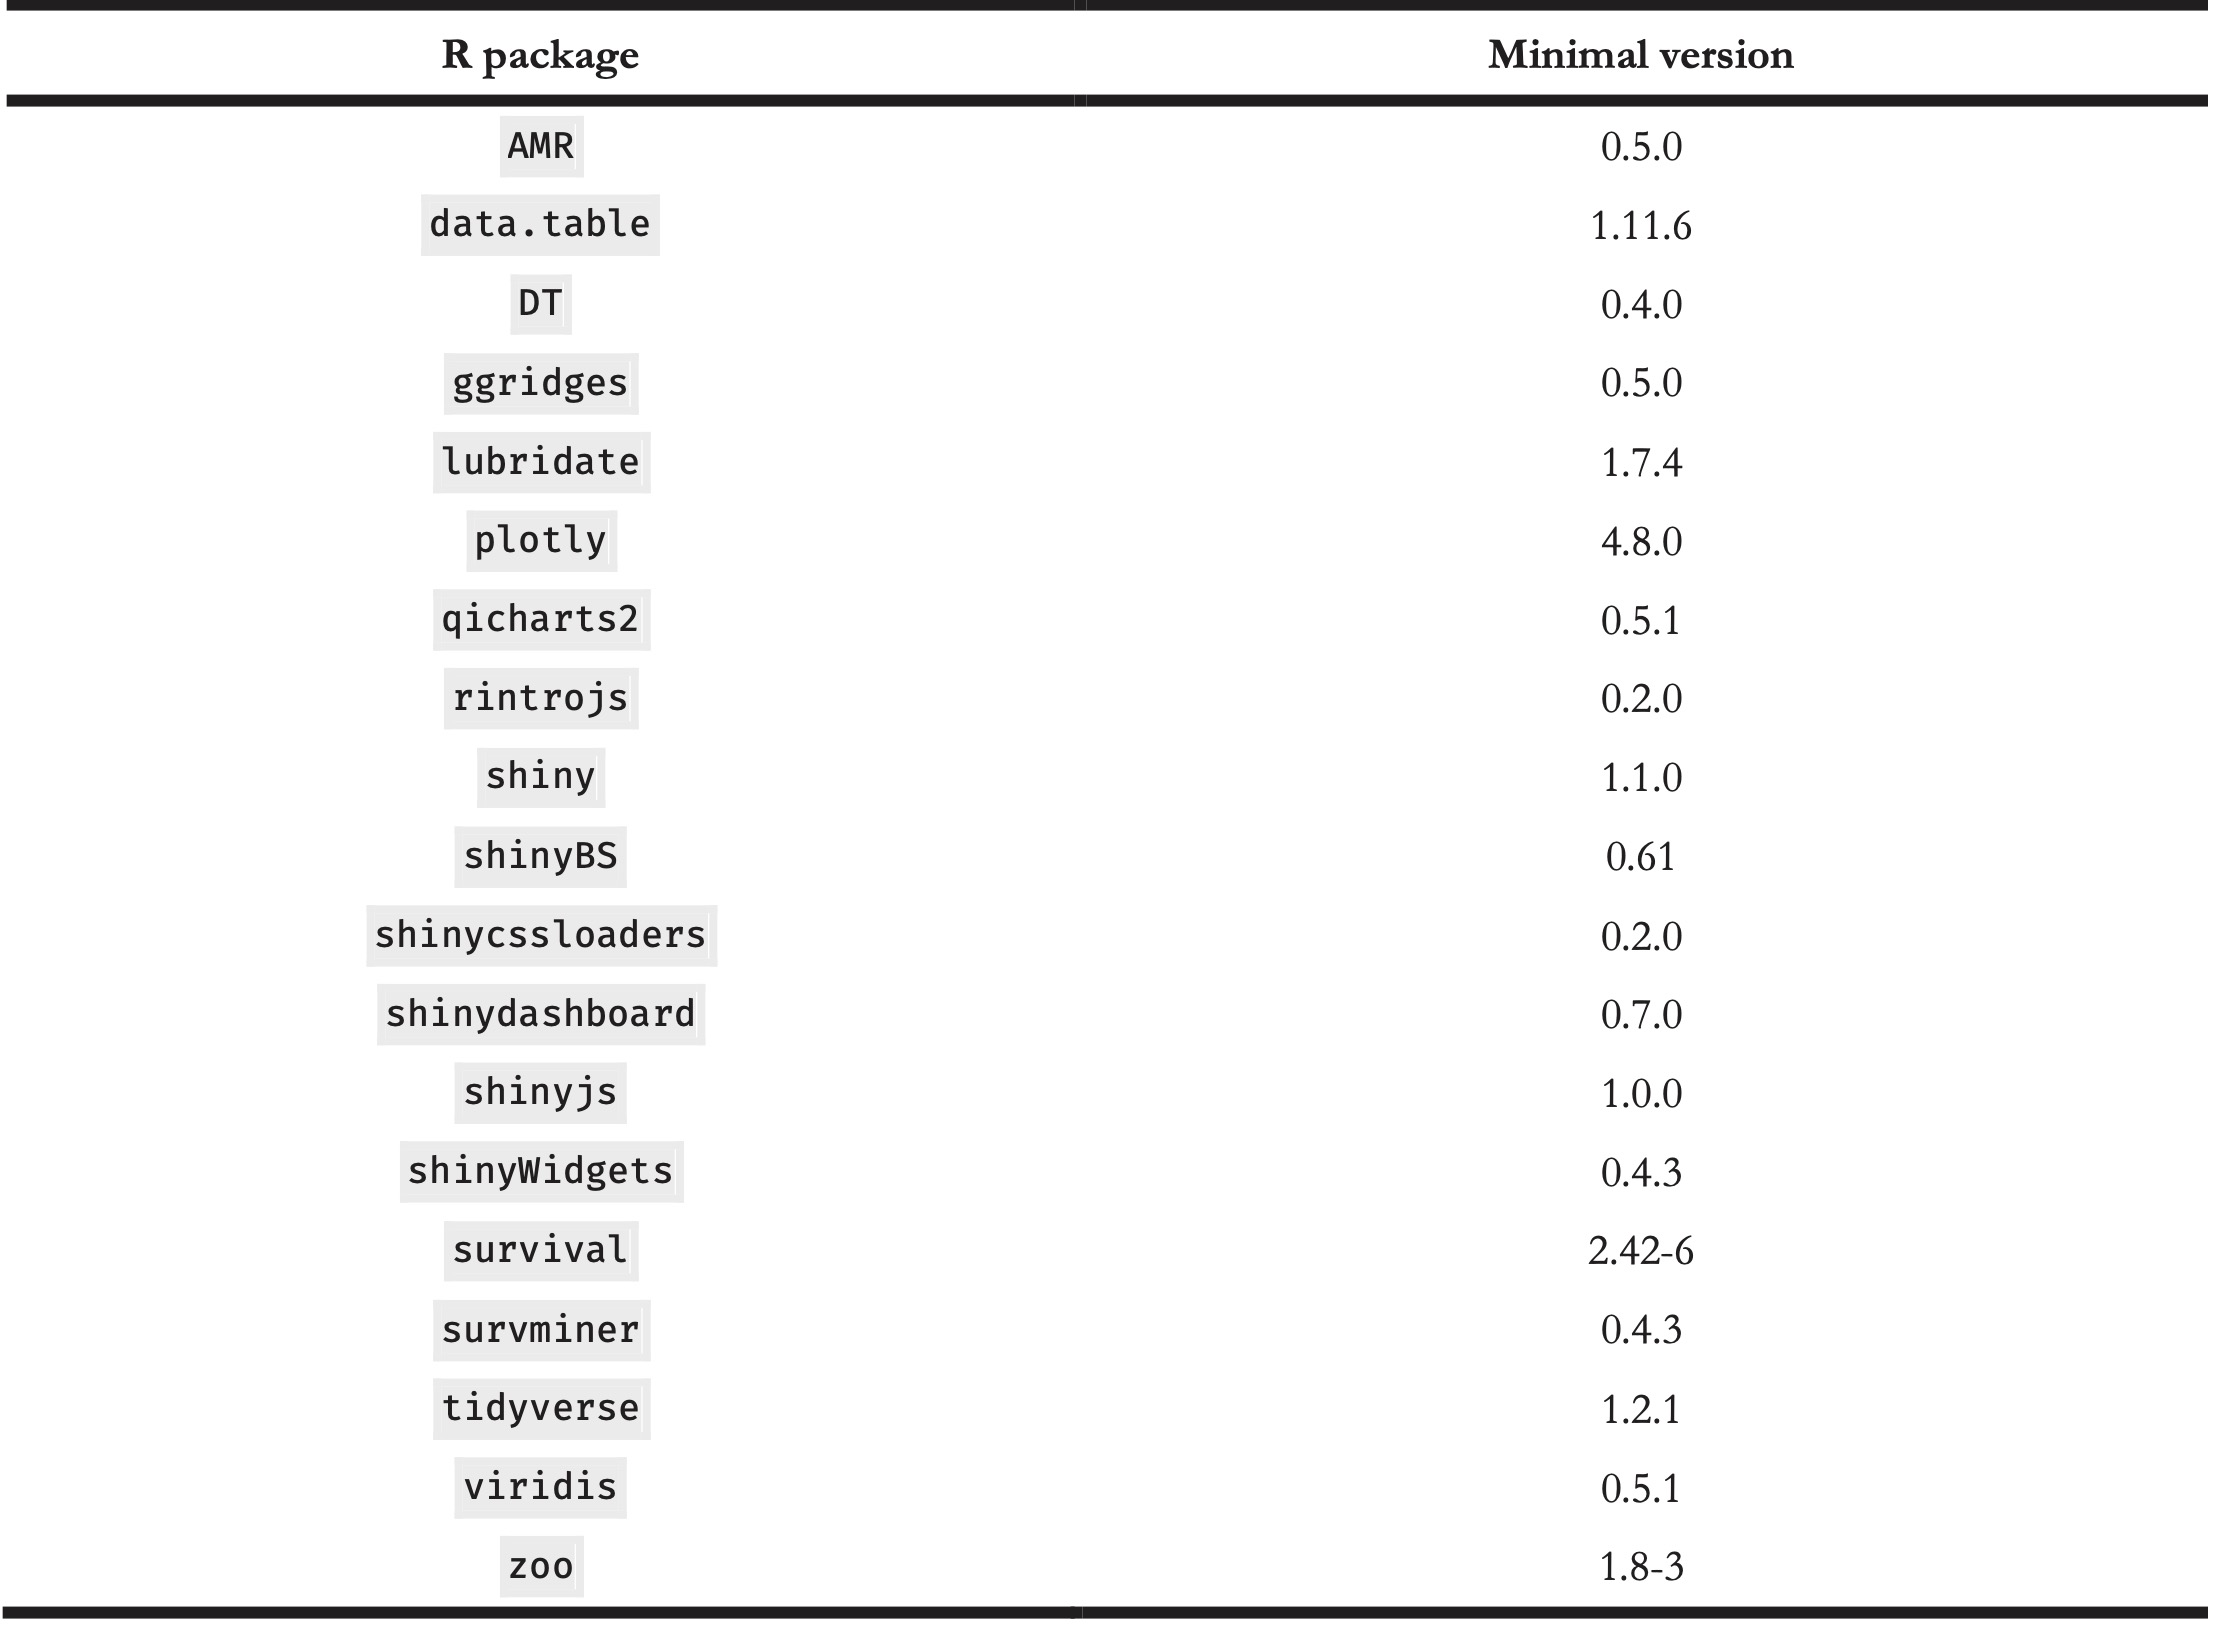
\includegraphics[width=1\linewidth]{images/05-t01} 

}

\end{figure}

The input data should be structured in a dataset format, where each variable is one column and each observation is one row. This follows the concept of ``tidy data,'' as defined by Hadley Wickham \textsuperscript{{[}26{]}}. Table 2 displays the set of variables underlying RadaR's functionality. In our setting for the development of RadaR, these variables originated from three different data sources: administrative data from the hospital data warehouse, microbiological data from the laboratory information system, and antimicrobial prescription data from the computerised prescriber order entry system. The data preparation and cleaning process are very specific for each data source, dependent on local data standards, and difficult to generalise. Therefore, Table 2 represents the final variables and formats for the analysis and use with RadaR, referring to the ``tidy data'' concept above and to the \texttt{R} package collection tidyverse for the preparation process \textsuperscript{{[}26,27{]}}. Additional variables are calculated and transformed using the packages lubridate and zoo for time points and intervals, and AMR for antimicrobial (group) names, microbial isolate names, first isolate identification, and resistance analysis \textsuperscript{{[}28-30{]}}. Microbiological resistance is calculated per antimicrobial substance or as co-resistance if more than one substance is selected.

Table 2. Input variables for RadaR.

\begin{figure}

{\centering 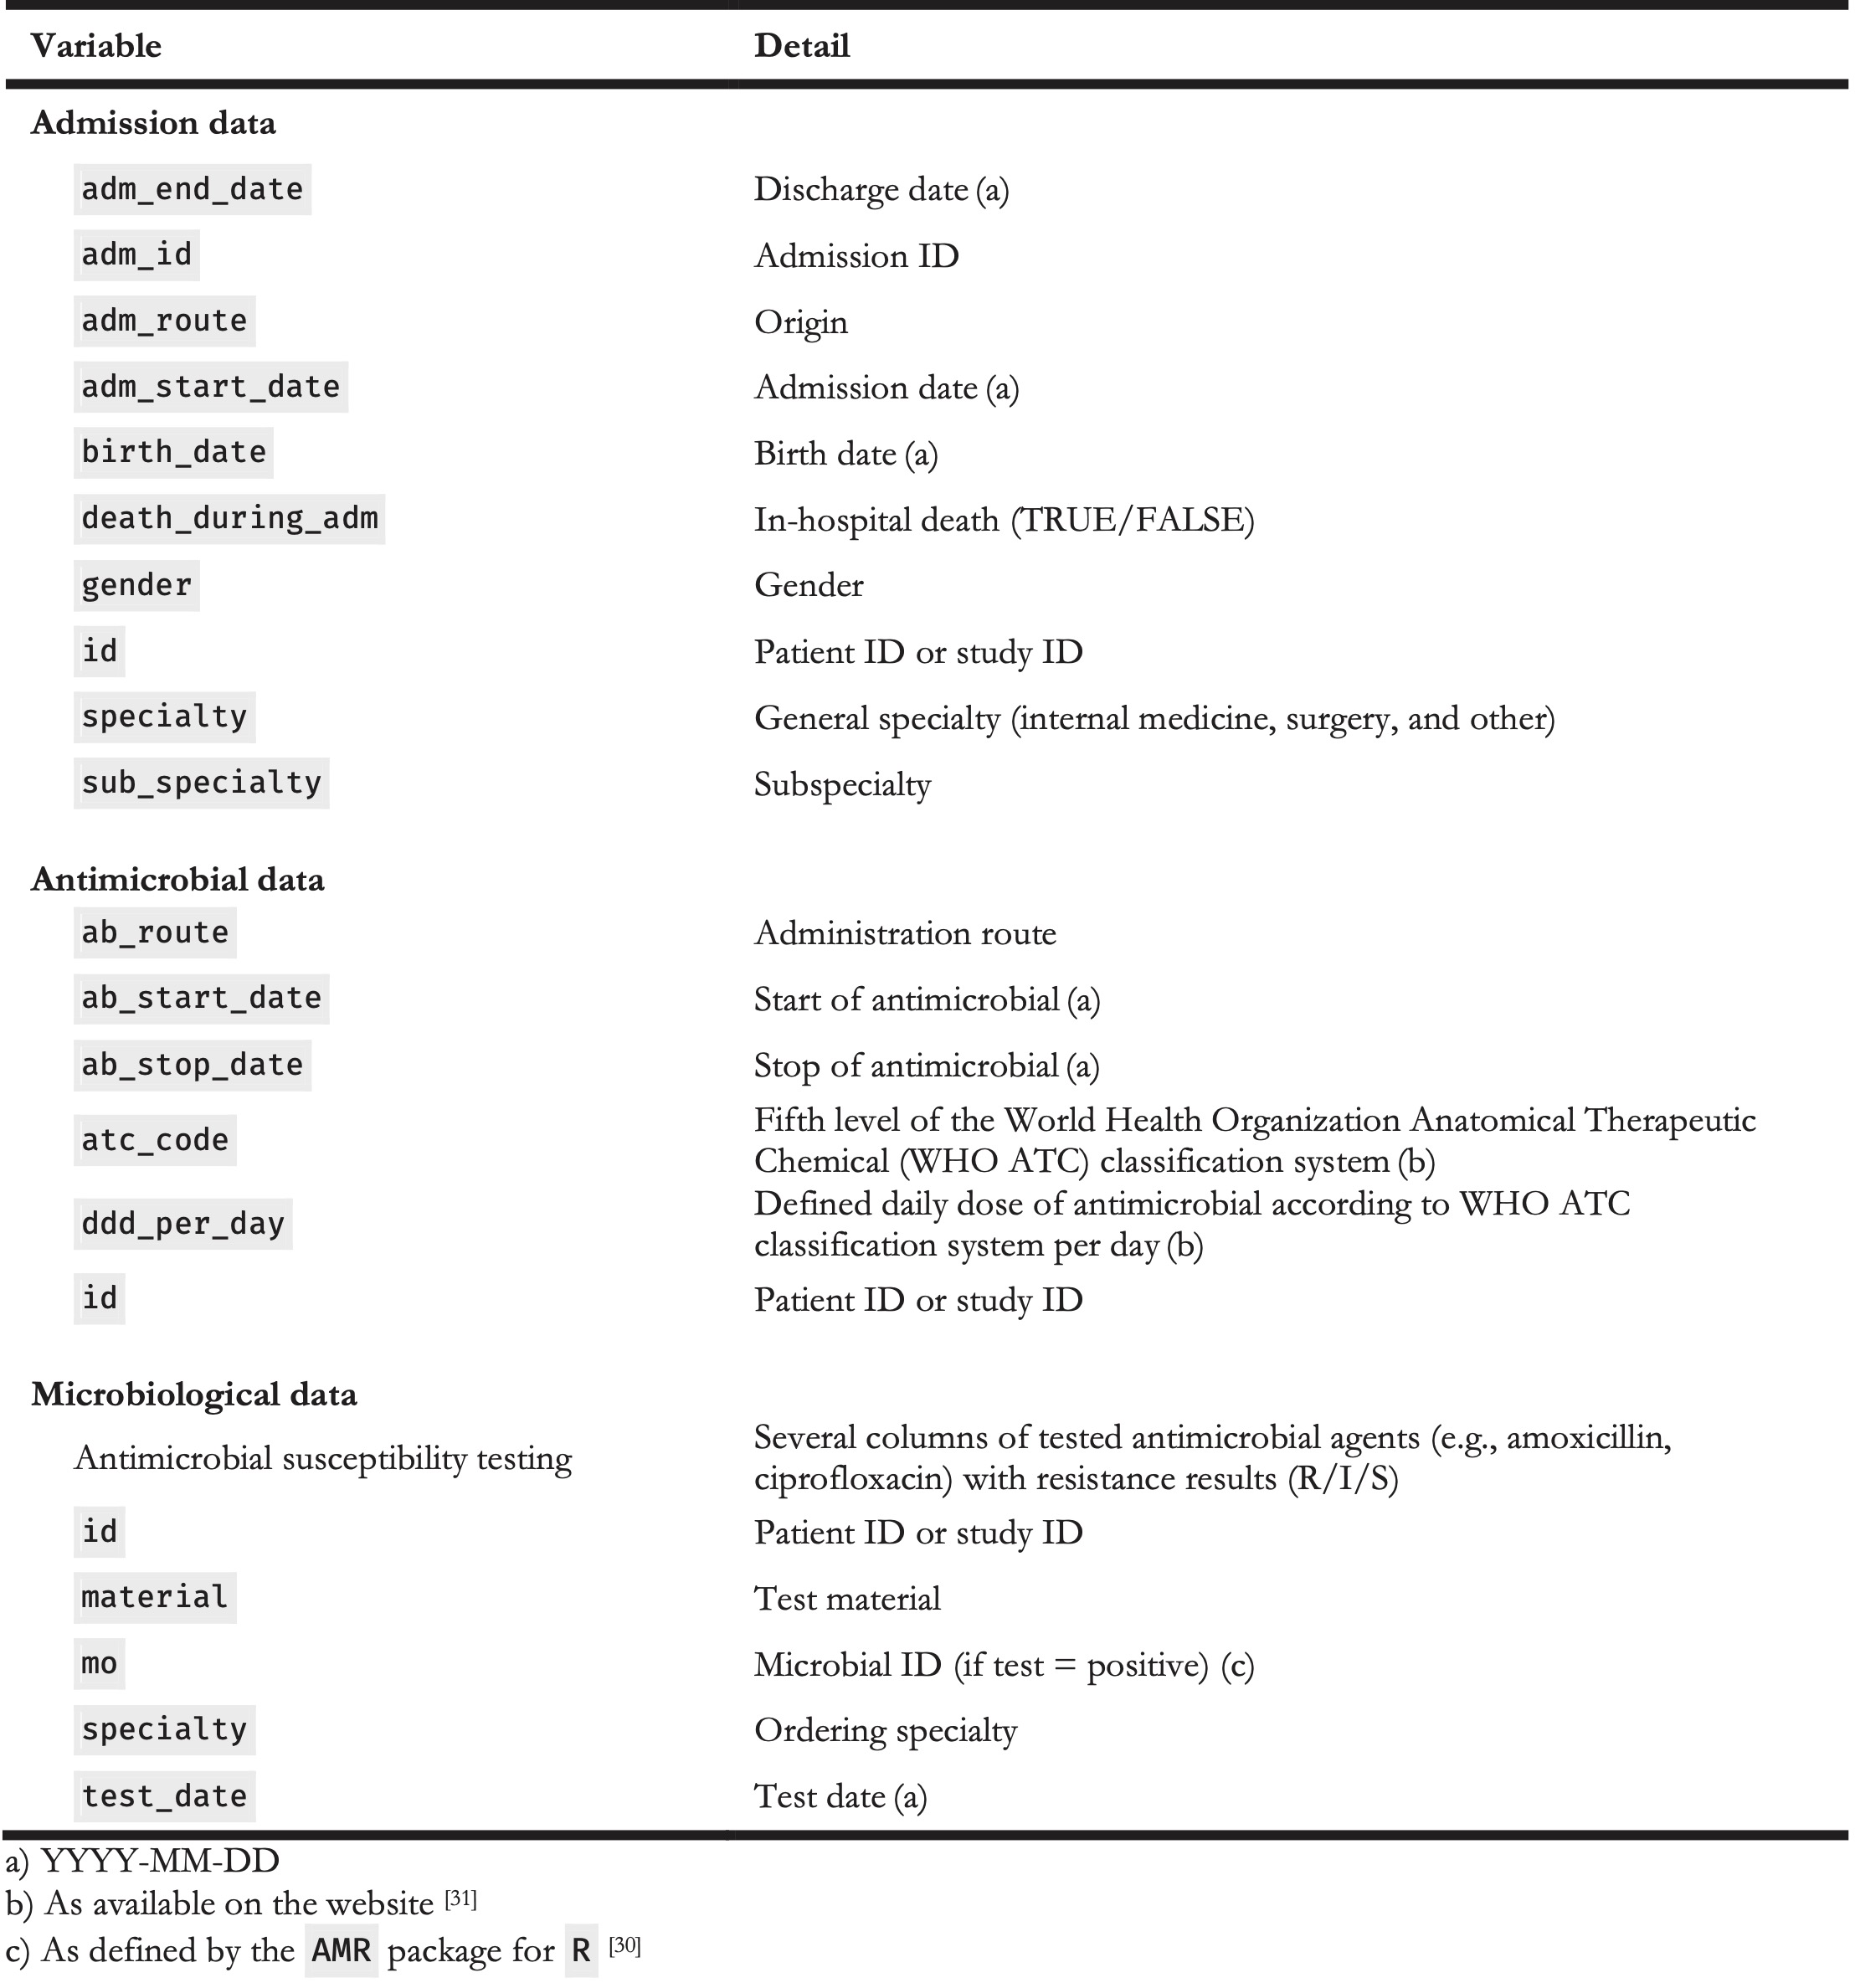
\includegraphics[width=1\linewidth]{images/05-t02} 

}

\end{figure}

The input data should be structured in a dataset format, where each variable is one column and each observation is one row. This follows the concept of ``tidy data,'' as defined by Hadley Wickham \textsuperscript{{[}26{]}}. Table 2 displays the set of variables underlying RadaR's functionality. In our setting for the development of RadaR, these variables originated from three different data sources: administrative data from the hospital data warehouse, microbiological data from the laboratory information system, and antimicrobial prescription data from the computerised prescriber order entry system. The data preparation and cleaning process are very specific for each data source, dependent on local data standards, and difficult to generalise. Therefore, Table 2 represents the final variables and formats for the analysis and use with RadaR, referring to the ``tidy data'' concept above and to the \texttt{R} package collection tidyverse for the preparation process \textsuperscript{{[}26,27{]}}. Additional variables are calculated and transformed using the packages lubridate and zoo for time points and intervals, and AMR for antimicrobial (group) names, microbial isolate names, first isolate identification, and resistance analysis \textsuperscript{{[}28-30{]}}. Microbiological resistance is calculated per antimicrobial substance or as co-resistance if more than one substance is selected.

RadaR can be used for graphical exploratory data analysis. Differences in LOS are displayed by a Kaplan-Meier curve in conjunction with a log-rank test, using the survminer package \textsuperscript{{[}32{]}}. Time trends for number of admissions, antimicrobial consumption, and resistance counts per year, quarter, or month, are visualised in run charts using the qicharts2 package \textsuperscript{{[}33{]}}. Nonrandom variation in these run charts is tested using Anhøj's rules \textsuperscript{{[}34{]}}.

RadaR has been developed in macOS High Sierra (1.4 GHz, 4 GB RAM), and it was successfully tested in Windows 7 (3.2 GHz, 8 GB RAM) and Linux (Ubuntu 16.04.4 LTS, 3.4 GHz, 12 GB RAM). A running example version has been deployed to shinyapps.io, a publicly available web hosting service for \texttt{R} Shiny apps \textsuperscript{{[}35{]}}. The entire source code of RadaR is freely accessible on GitHub \textsuperscript{{[}36{]}}. We intend to integrate suggestions and feedback coming from its users and the \texttt{R} community. RadaR was developed using data of patients admitted to the University Medical Center Groningen, Groningen, the Netherlands. Data were collected retrospectively, and permission was granted by the ethical committee (METc 2014/530). RadaR can be used locally in protected environments or hosted on the web, provided appropriate measures have been taken to guarantee data protection, depending on national regulations.

\hypertarget{results}{%
\section{Results}\label{results}}

\hypertarget{overview}{%
\subsection{Overview}\label{overview}}

We have developed RadaR, a web-based software app providing an intuitive platform for rapid analysis of large datasets containing information about patients' admission, antimicrobial use, and results of microbiological diagnostic tests. This software app can help users (i.e., AMS team members) find answers to questions, such as ``What are the most commonly used antimicrobials at an institution/specialty/department and have they changed over time?'', ``Were adequate microbiological diagnostics performed at the start of antimicrobial treatments?'', ``What are the most frequent microorganisms found and their resistance patterns in different departments?'', and ``Can we identify priority areas within a hospital where antimicrobial or microbiological diagnostic use has the largest room for improvement?''.

\hypertarget{application-design}{%
\subsection{Application Design}\label{application-design}}

RadaR is designed in the form of a web browser--based dashboard that most users are familiar with from typical websites and web-based tools (see Figure 1). The basis of RadaR's functionality is filtering datasets and producing analytical graphs according to selection criteria defined by the user. Any calculations and data aggregation are based on single observations of individual patients. To identify and analyse groups of patients, 17 different selection criteria can be found in the sidebar (Table 3). The output of RadaR is grouped into four panels (patient, antimicrobials, diagnostics, and outcome) that each comprise three to four output boxes displaying the results.

Table 3. Selection criteria in sidebar.

\begin{figure}

{\centering 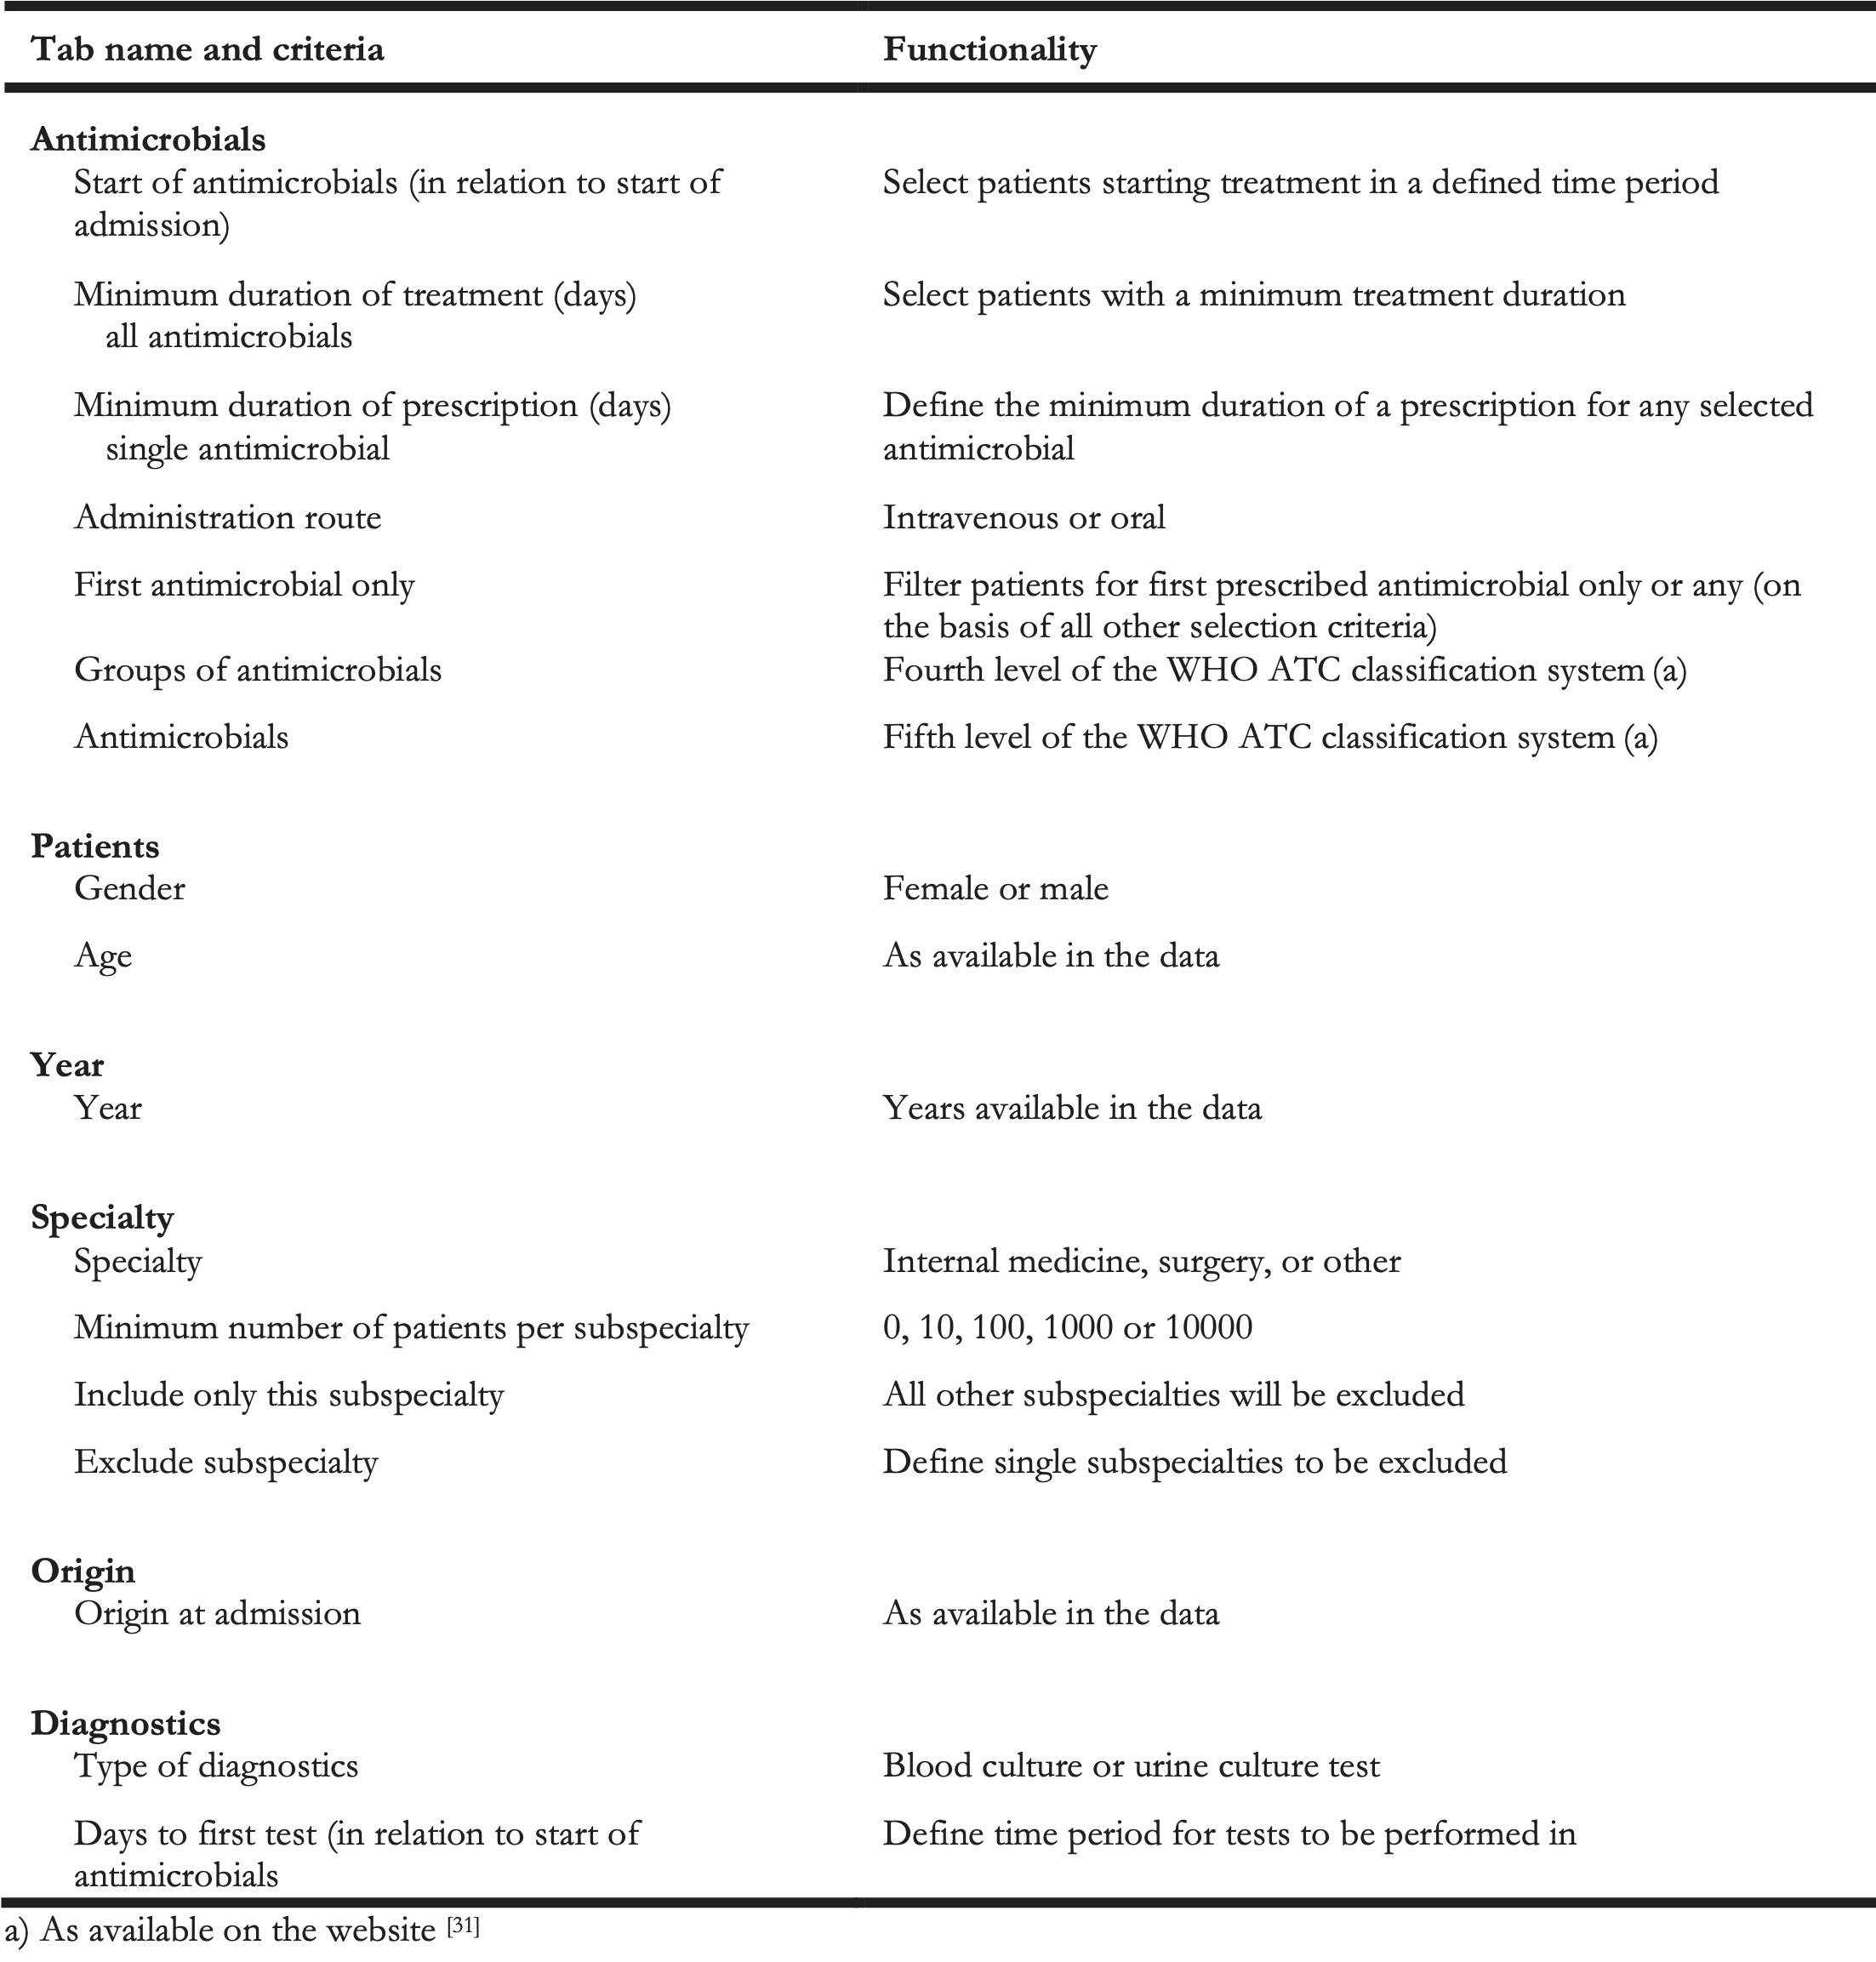
\includegraphics[width=1\linewidth]{images/05-t03} 

}

\end{figure}

All output is based on the selection criteria defined by the user in the sidebar. Each new selection and any change need to be confirmed by clicking the confirm selection button (see Figure 1). Users can navigate among the different analysis panels by clicking the respective button.

\begin{figure}

{\centering 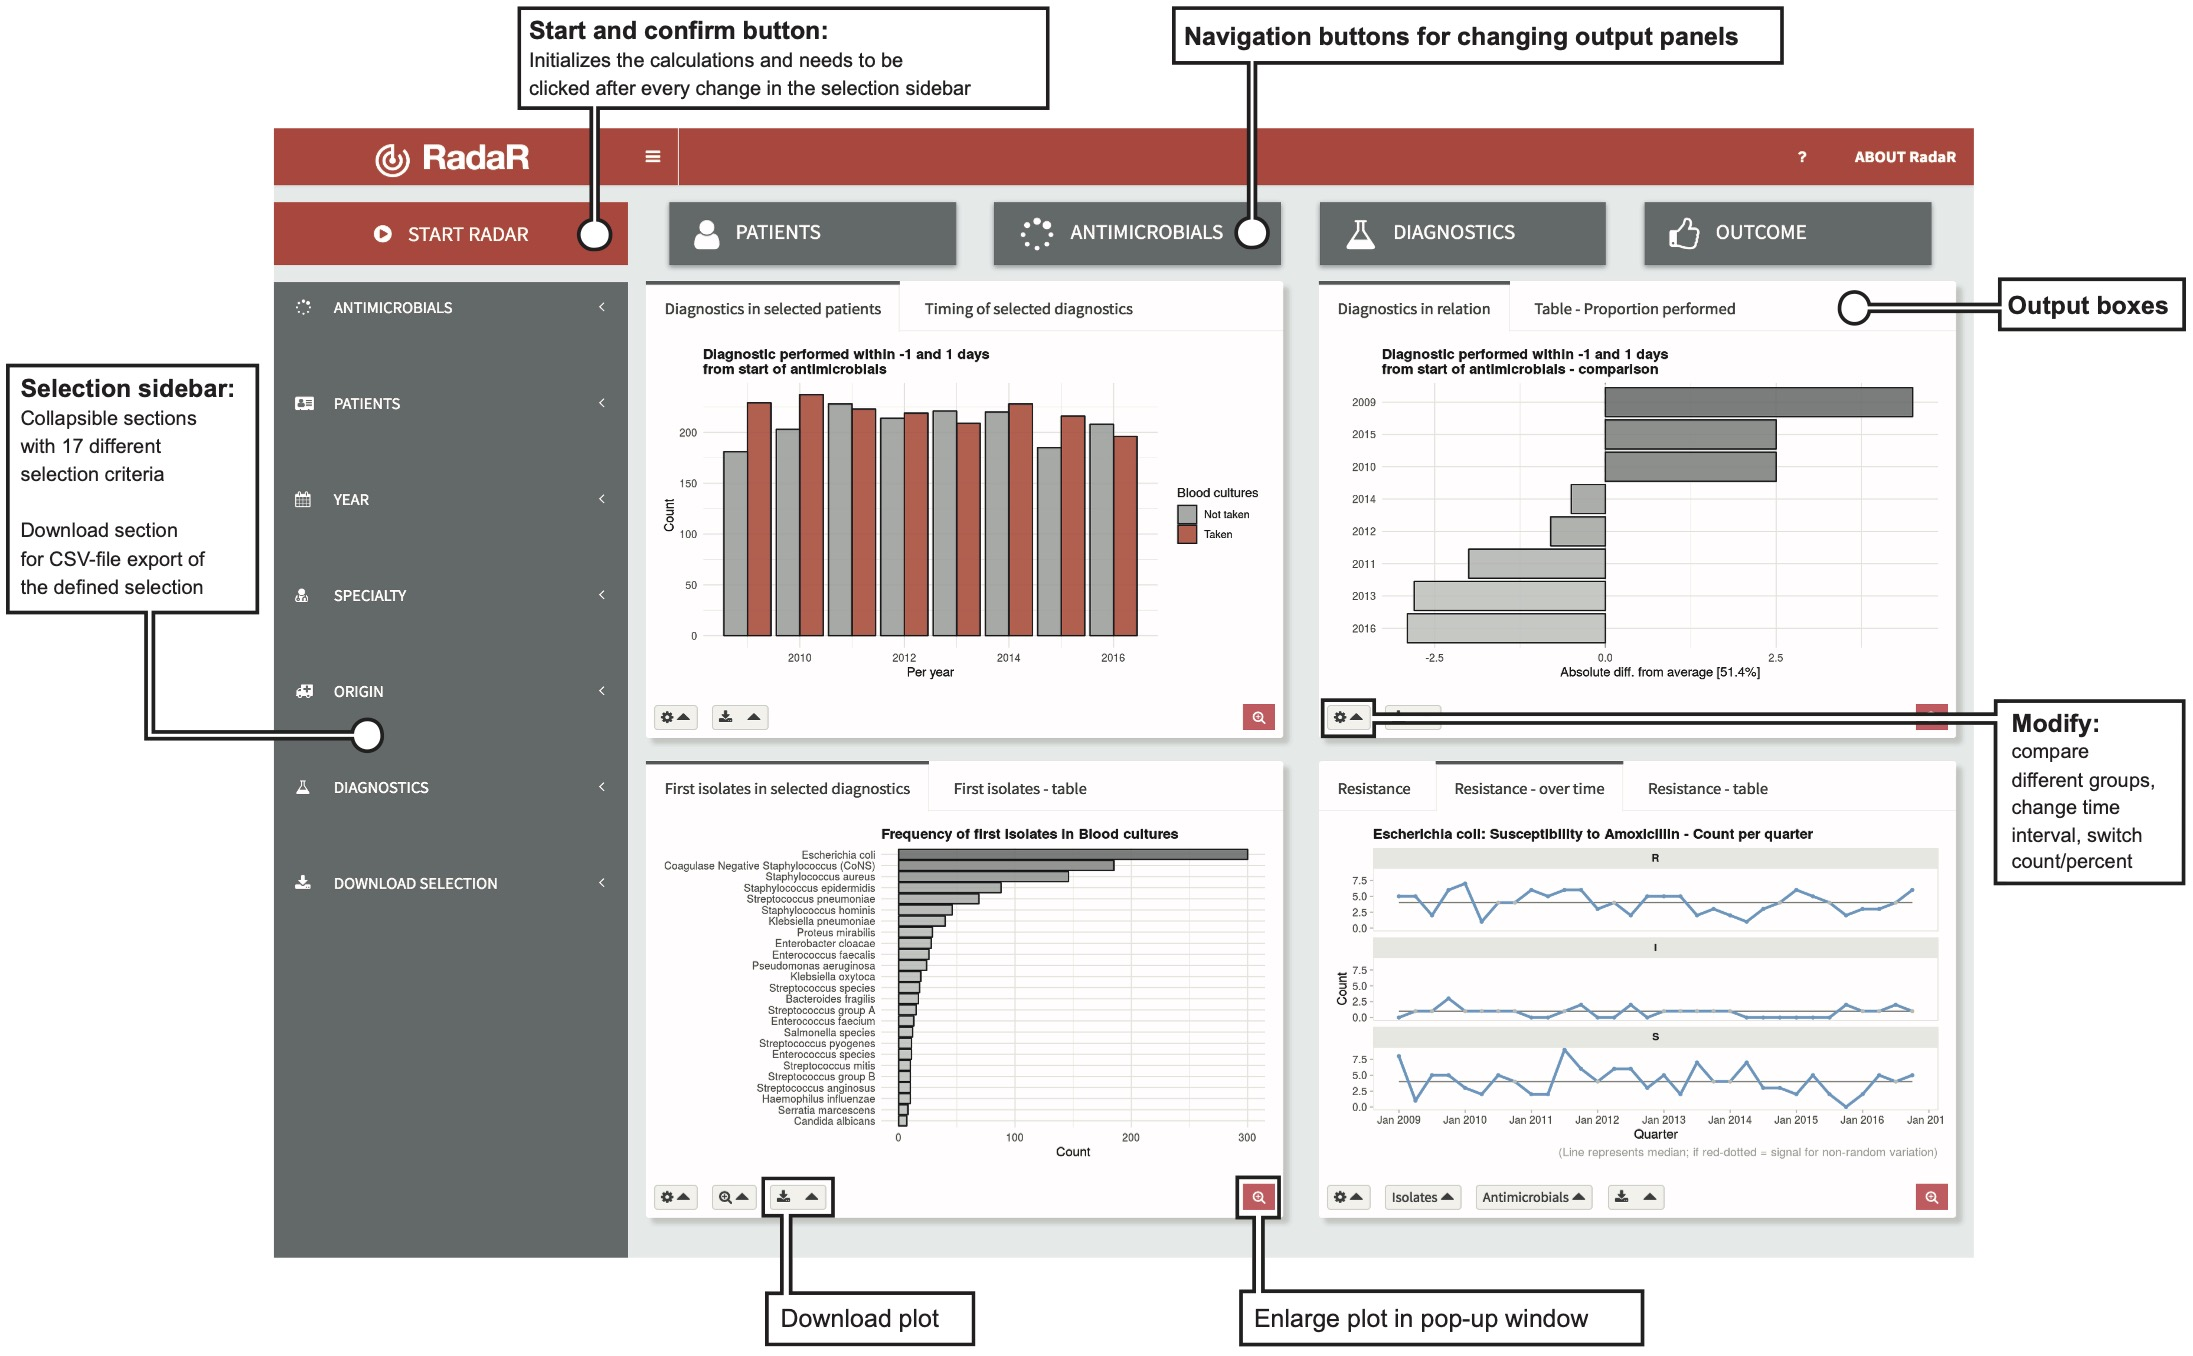
\includegraphics[width=1\linewidth]{images/05-01} 

}

\caption{Application design.}\label{fig:fig5-1}
\end{figure}

Results are shown in bar charts, density plots, run charts, a bubble plot, and a Kaplan-Meier curve for LOS in hospital. Each panel further displays a table summarizing the respective data analyses. All output boxes and their content are described in Table 4. Most output boxes include modification options that can be identified by small gear icons (see Figure 1). These clickable icons allow for further specification of the generated plots and tables. Users can compare different groups (e.g., antimicrobial use by antimicrobial agent, resistance patterns per isolate, or LOS by specialty) or modify the plots (e.g., switch from count to proportion, change the chart type, or show or hide the legend). Plots and tables can be downloaded through download buttons as PNG files for plots and CSV, Excel, or PDF files for tables.

Table 4. Output boxes for analysis results.

\begin{figure}

{\centering 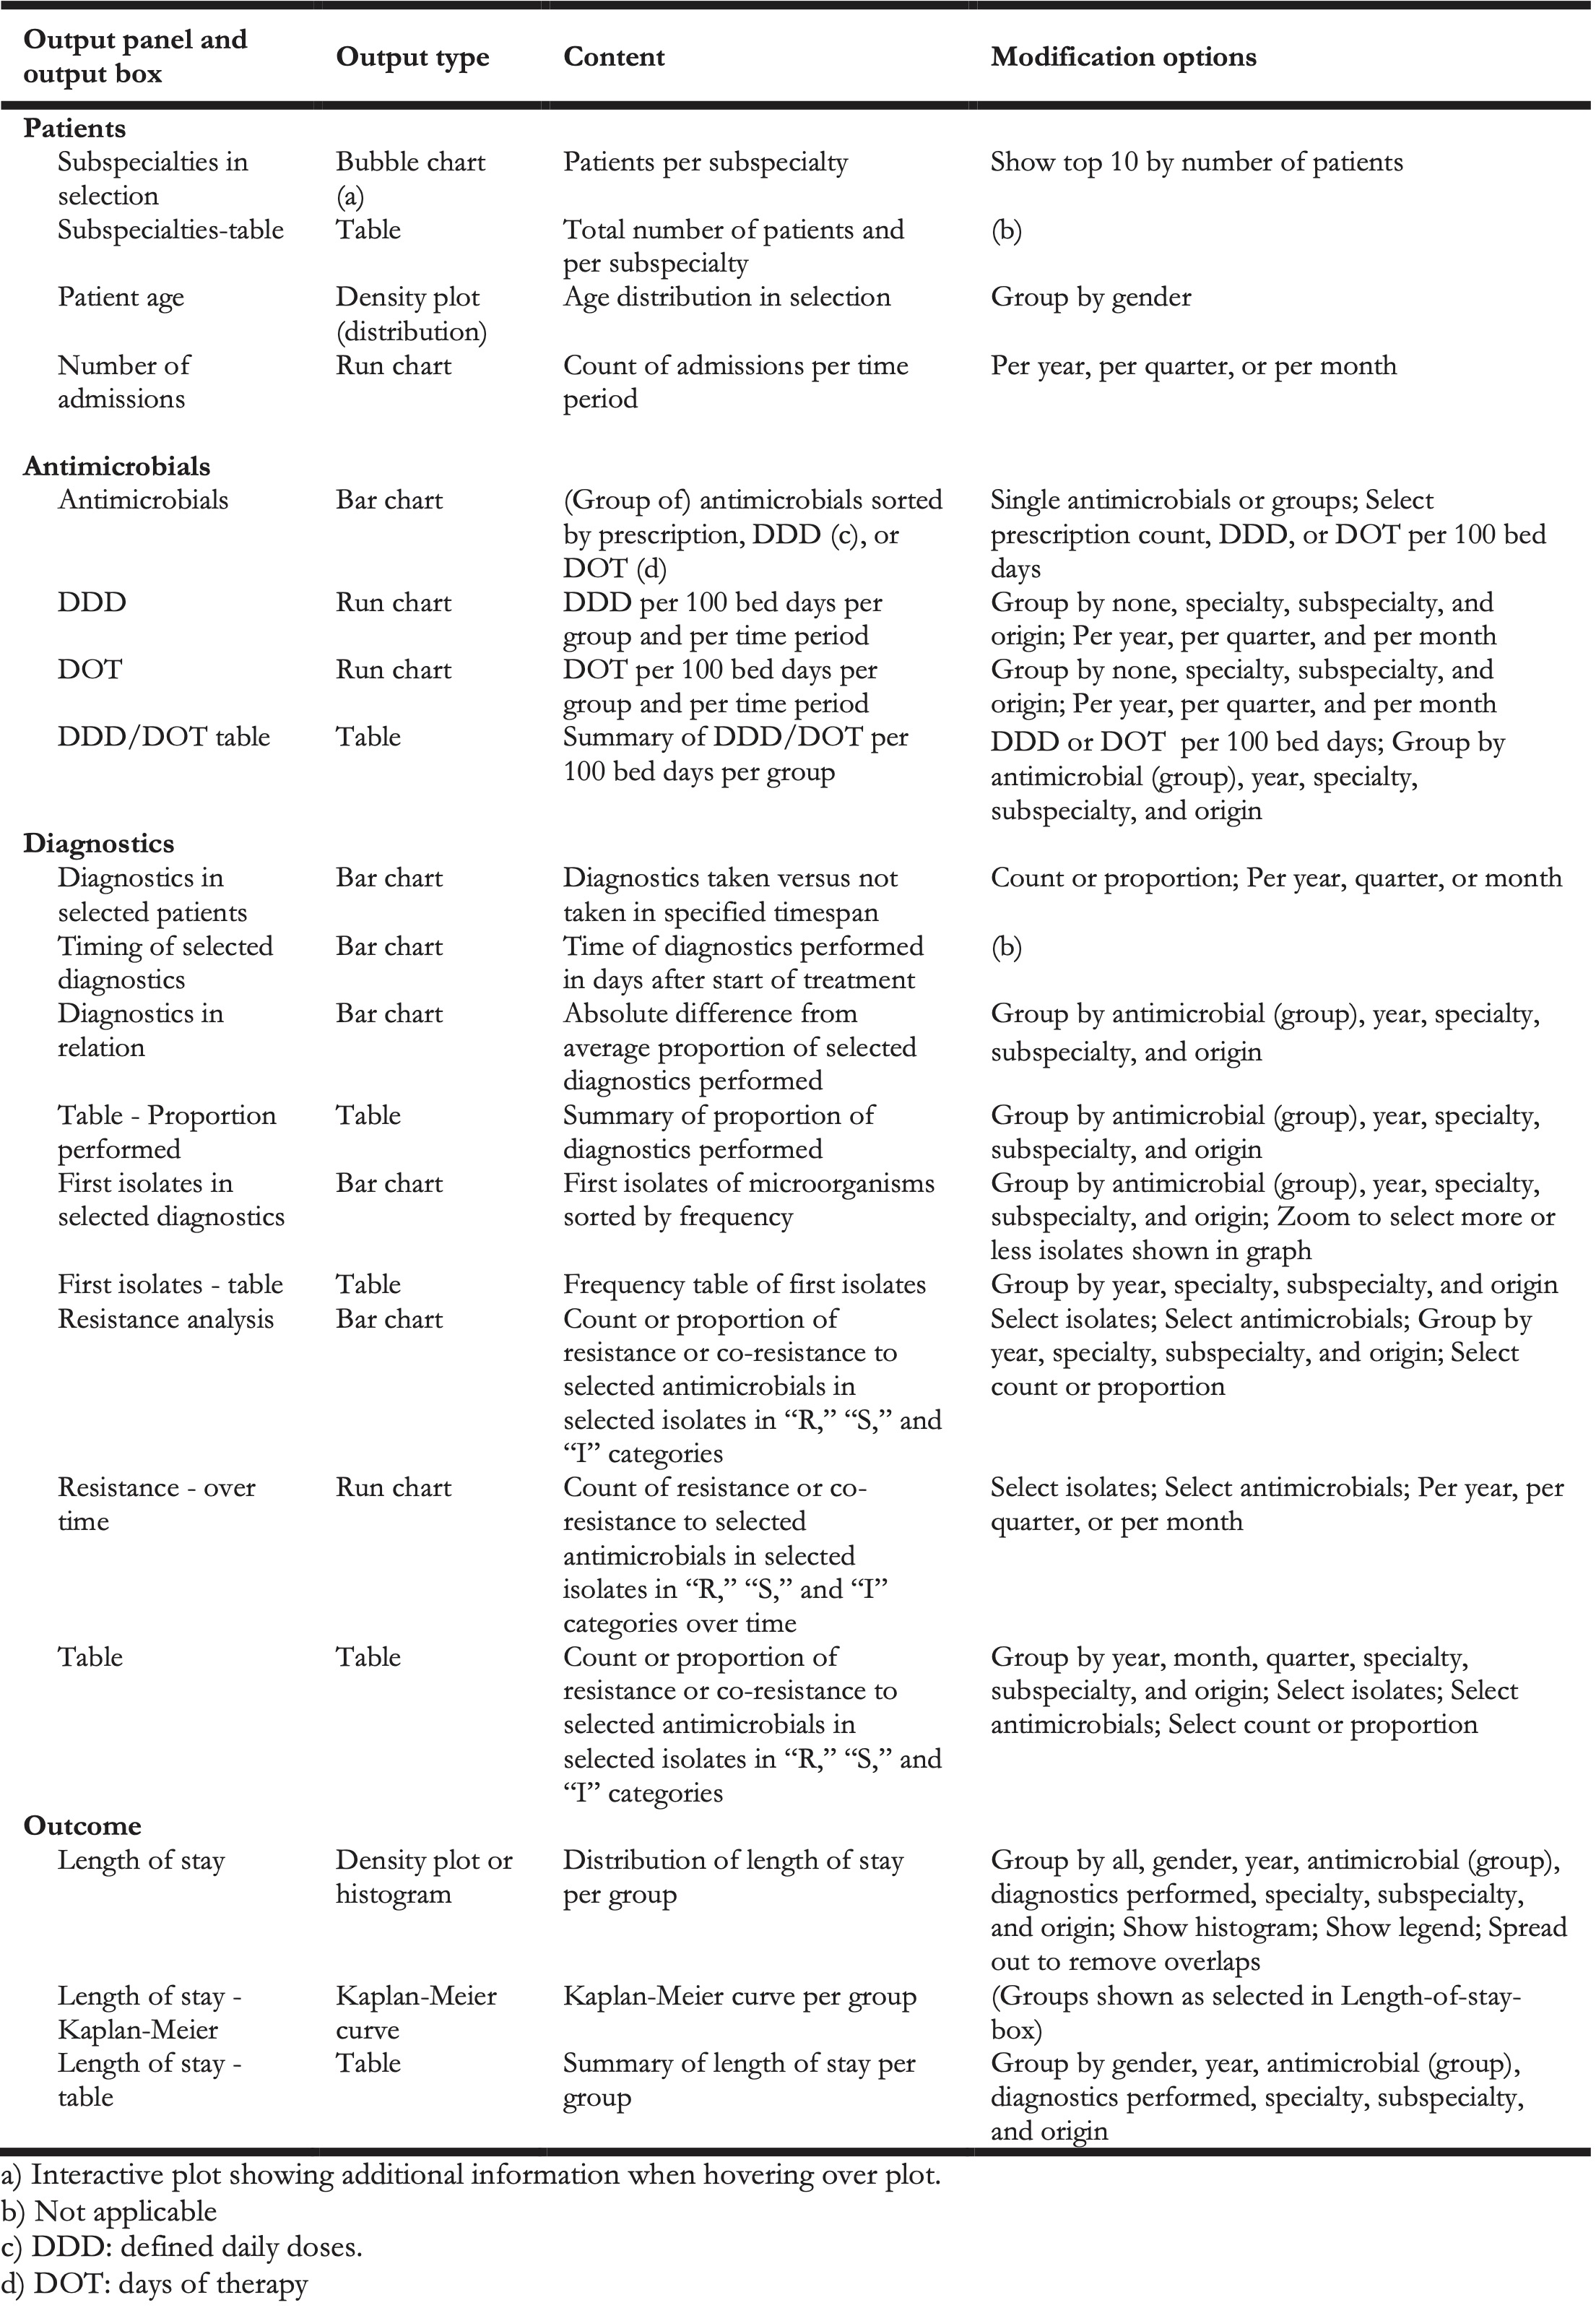
\includegraphics[width=1\linewidth]{images/05-t04} 

}

\end{figure}

Finally, two datasets (antimicrobial/admission data and microbiological data) of the user-defined selection can be downloaded from the sidebar menu in a CSV-file format for further analysis (e.g., retrieving a list of patient numbers of the selected patient group).

\hypertarget{development-process}{%
\subsection{Development Process}\label{development-process}}

RadaR has been developed in close contact with the AMS team and senior consulting specialists at the University Medical Center Groningen, Groningen, the Netherlands, to meet the needs and requirements of this user group. Subsequently, all members of the European Society of Clinical Microbiology and Infectious Diseases Study Group for Antimicrobial Stewardship (ESGAP) were asked to evaluate and test the software app through a running web-based example of RadaR and by filling out a web-based survey. The ESGAP comprises around 200 members from more than 30 countries worldwide. A total of 12 members from 9 different countries took part in the evaluation. This yielded important information on user experiences with the software app, which in turn led to further improvements that are reflected in the version we presented in this report. In a next phase, RadaR will be tested in different settings of ESGAP members and other interested partners using locally available data (e.g., an 837-bed tertiary care hospital in the Netherlands and a 750-bed tertiary care hospital in Greece).

\hypertarget{workflow}{%
\subsection{Workflow}\label{workflow}}

RadaR was developed and tested with a dataset of all patients admitted to our institution, a 1339-bed academic tertiary referral hospital, within the years of 2009 to 2016, comprising over 180,000 admissions. For simulation purposes and web-based user testing, we have created a test dataset of 60,000 simulated patients. This sample dataset allows testing of RadaR's functionality, but it does not produce meaningful results.

A typical example workflow with RadaR comprises 6 steps (with examples from the test dataset). They are listed below:

\begin{enumerate}
\def\labelenumi{\arabic{enumi}.}
\tightlist
\item
  Define the selection: For example, patients receiving intravenous second- or third-generation cephalosporins as first treatment for at least two days, starting within the first two days of hospital admission from any specialty in all years in the dataset.
\item
  Patients' panel: Identify the total number of patients and the subspecialties with the highest number of included patients (e.g., 537 patients selected in total, with 97 patients from internal medicine). Investigate patients' gender and age distribution.
\item
  Antimicrobials panel: Identify the total use of the initial cefuroxime treatment in DDD and DOT per 100 bed days (e.g., 4.51 and 1.5, respectively). Stratify the results by subspecialty and identify the highest number of DDD and DOT per 100 bed days (e.g., highest use by DDD and DOT in internal medicine).
\item
  Diagnostics panel: Check if the selected microbiological diagnostic test (e.g., blood culture test) has been performed on the same day as the start of the treatment (defined in the sidebar). Investigate the proportion of tests performed over the years and investigate which subspecialty performs best compared with others (e.g., paediatrics). Check which microorganisms (as first isolates) were found in the selected diagnostic specimens (the most common isolate: Escherichia coli). Investigate the proportion of isolates resistant to cefuroxime (8.9\%) and analyse the trend over time.
\item
  Outcome panel: Check for patterns of differences in LOS in the defined patient group by subspecialties or performed diagnostics (e.g., highest mean LOS of 7.8 days in Surgery).
\item
  Refine the selection: Investigate a subgroup of the original selection. For example, select only the top three subspecialties by number of patients and repeat step 2 to 5.
\end{enumerate}

\hypertarget{customisation}{%
\subsection{Customisation}\label{customisation}}

For setting up RadaR in a new environment after data preparation, users only need to perform the following four steps:

\begin{enumerate}
\def\labelenumi{\arabic{enumi}.}
\tightlist
\item
  Downloading \texttt{R} and RStudio \textsuperscript{{[}21,22{]}}, which are free to use and open-source software
\item
  Download or copy and paste RadaR's source code \textsuperscript{{[}36{]}} into three files in RStudio -- \texttt{global.R}, \texttt{server.R}, and \texttt{ui.R}
\item
  In \texttt{global.R}, manually edit the paths for the prepared datasets to be imported into RadaR
\item
  Run the app in RStudio with the calling the function \texttt{runApp()} in the console or by clicking the green run app button. This will download and install the required \texttt{R} packages needed for the app if they have not been installed previously, and this will create the final dataset for analysis. The RadaR interface will open in the RStudio viewer pane or in a new window of the standard browser of the user's operating system.
\end{enumerate}

RadaR's appearance has been customised using a cascading style sheets (CSS) script \textsuperscript{{[}37{]}} that is loaded into the app upon its start. This script needs to be saved into a subdirectory of the directory of the three main files (\texttt{global.R}, \texttt{server.R}, and \texttt{ui.R}) called \texttt{www}. We recommend RStudio's project function to create a single project for RadaR and to store all information in this project directory. Users with experience in using CSS can fully alter RadaR's design by changing the underlying CSS script.

\hypertarget{discussion-1}{%
\section{Discussion}\label{discussion-1}}

\hypertarget{principal-findings}{%
\subsection{Principal Findings}\label{principal-findings}}

We have developed a web-based software app for rapid analysis of diagnostic and antimicrobial patterns that can support AMS teams to tailor their interventions. It has been designed to enhance communication of relevant findings while being easy to use. This also applies to users without extensive prior software skills, as it follows usual web browser user experiences. Moreover, it has been developed using open-source software. It is therefore free to use and accessible for download. In our experience, this system can be adapted to new settings within one day, when the required data (Table 2) are available.

Commercial software for infection management is available (e.g., Epic Antimicrobial Stewardship Module, TREAT Steward). These offer extensive options for filtering, analysing, and visualizing EHRs with real-time connections to hospital data infrastructures and have been shown to be useful in clinical practice \textsuperscript{{[}38{]}}. However, it is difficult to compare functionalities of these tools because of their non--open-source nature. This fact, along with the required budget to purchase the software, drastically limits their use. We are convinced that transparent software development can support the adoption of data-driven developments while enhancing optimal quality of care and patient safety, which is crucial in the light of new data-driven developments of using EHRs \textsuperscript{{[}39,40{]}}.

The global nature of infections further calls to develop software tools applicable in resource-limited settings \textsuperscript{{[}41{]}}. Open-source approaches for data analysis, such as RadaR, have advantages over traditional methods, such as Excel or SPSS. Hughes et al described those in their report of a software app for RNA-sequencing data analysis \textsuperscript{{[}15{]}}. They highlight aspects that were also fundamental for the development of RadaR. First, \texttt{R} allows transparent, reproducible, and sustainable data analysis through scripts that can easily be shared and changed. This can build the basis for collaboration, and this enforces the spirit of open science (also through the strong collaborative \texttt{R} community on the web). Second, \texttt{R} is open source and free to use; therefore, it also enables use in resource-limited settings. Finally, Shiny empowers users to interact with the data, making even very large datasets quickly interpretable.

Innovative approaches used in supporting infection management by leveraging EHRs are being investigated \textsuperscript{{[}17-19{]}}. Reporting on AMR, antimicrobial use, and hospital infections (e.g., for quality assurance) is well established, but it is important to integrate these data sources in an approach that allows detailed filtering options on all input. Merely looking at antimicrobial use alone or comparing aggregated results (e.g., total amount of a specific antimicrobial substance per hospital correlated with the total count of a resistant isolate) will result in loss of information or even misleading interpretation. Detailed data and calculations on the basis of each individual patient are crucial to draw informed conclusions. Unfortunately, the abovementioned infection management approaches \textsuperscript{{[}17-19{]}} either depend on additional commercial software for data visualisation or the source code is not openly available. We want to encourage others to turn toward available open-source software solutions, such as R, for an increased potential of collaboration and transparency. However, their strength is the connection to real-time data flows. This enables the prospective use and increases their usability for daily clinical practice. RadaR is currently still limited to retrospective data analysis because of a changing hospital data infrastructure in our setting. Technically, it is feasible to connect R-based software apps such as RadaR to real-time hospital data infrastructures running with clinical data standards \textsuperscript{{[}42{]}}. For a start, access to static data extraction is often easier and faster to achieve. RadaR can be used to advocate the use of data visualisation tools and improved accessibility of hospital data sources. Until connection to real-time hospital data is established, RadaR can support users as a stand-alone option for retrospective data analysis in infection management. Next steps will involve testing in multiple settings and forming a user and research group to continue and expand the use of open-source technology and open science principles in infection management.

\hypertarget{conclusions}{%
\subsection{Conclusions}\label{conclusions}}

RadaR demonstrates the feasibility of developing software tools for infection management and AMS teams in an open-source approach, making it free to use, share, or modify according to various needs in different settings. RadaR has the potential to be a highly useful tool for infection management and AMS in daily practice.

\hypertarget{acknowledgements-1}{%
\section*{Acknowledgements}\label{acknowledgements-1}}
\addcontentsline{toc}{section}{Acknowledgements}

The authors would like to thank the ESGAP executive committee for supporting the evaluation of RadaR in the ESGAP study group and all its members for their valuable input, suggestions, and comments. Furthermore, the authors wish to thank Igor van der Weide, Jan Arends, and Prashant Nannan Panday for their great support in obtaining required data at our institution that built the basis for the development of RadaR. The authors also thank the online \texttt{R} community as well as the valuable comments, suggestions, and input from reviewers that they have received to improve RadaR.

RadaR was developed as part of a project funded by the European Commission Horizon 2020 Framework Marie Skłodowska-Curie Actions (grant agreement number: 713660-PRONKJEWAIL-H2020-MSCA-COFUND-2015).

\hypertarget{conflicts-of-interests}{%
\section*{Conflicts of interests}\label{conflicts-of-interests}}
\addcontentsline{toc}{section}{Conflicts of interests}

None declared.

\hypertarget{references-4}{%
\section*{References}\label{references-4}}
\addcontentsline{toc}{section}{References}

\begin{enumerate}
\def\labelenumi{\arabic{enumi}.}
\tightlist
\item
  Dyar OJ, Huttner B, Schouten J, Pulcini C, ESGAP (ESCMID Study Group for Antimicrobial stewardshiP). What is antimicrobial stewardship? Clin Microbiol Infect 2017 Nov;23(11):793--798. \url{PMID:28882725}
\item
  Barlam TF, Cosgrove SE, Abbo LM, MacDougall C, Schuetz AN, Septimus EJ, Srinivasan A, Dellit TH, Falck-Ytter YT, Fishman NO, Hamilton CW, Jenkins TC, Lipsett PA, Malani PN, May LS, Moran GJ, Neuhauser MM, Newland JG, Ohl CA, Samore MH, Seo SK, Trivedi KK. Implementing an antibiotic stewardship program: Guidelines by the Infectious Diseases Society of America and the Society for Healthcare Epidemiology of America. Clin Infect Dis 2016 May 15;62(10):e51--77. \url{PMID:27080992}
\item
  Davey P, Marwick CA, Scott CL, Charani E, McNeil K, Brown E, Gould IM, Ramsay CR, Michie S. Interventions to improve antibiotic prescribing practices for hospital inpatients. Cochrane Database Syst Rev 2017 Feb 9;2:CD003543. \url{PMID:28178770}
\item
  National Institute for Health and Care Excellence. Antimicrobial stewardship: systems and processes for effective antimicrobial medicine use. \url{https://www.nice.org.uk/Guidance/NG15}. Archived at: \url{http://www.webcitation.org/73ybLqgCI}
\item
  Schuts EC, Hulscher MEJL, Mouton JW, Verduin CM, Stuart JWTC, Overdiek HWPM, van der Linden PD, Natsch S, Hertogh CMPM, Wolfs TFW, Schouten JA, Kullberg BJ, Prins JM. Current evidence on hospital antimicrobial stewardship objectives: a systematic review and meta-analysis. Lancet Infect Dis 2016 Jul;16(7):847--856. \url{PMID:26947617}
\item
  Stichting Werkgroep AntibioticaBeleid. SWAB Guidelines for Antimicrobial Stewardship 2016. \url{http://www.swab.nl/swab/cms3.nsf/uploads/FAF701FBF4FCBDD6C12580EC0037D292/$FILE/20161228\%20SWAB\%20Guidelines\%20for\%20Antimicrobial\%20Stewardship\%20-definitief.pdf} . Archived at: \url{http://www.webcitation.org/73ycxKUfO}
\item
  Pulcini C, Binda F, Lamkang AS, Trett A, Charani E, Goff DA, Harbarth S, Hinrichsen SL, Levy-Hara G, Mendelson M, Nathwani D, Gunturu R, Singh S, Srinivasan A, Thamlikitkul V, Thursky K, Vlieghe E, Wertheim H, Zeng M, Gandra S, Laxminarayan R. Developing core elements and checklist items for global hospital antimicrobial stewardship programmes: a consensus approach. Clin Microbiol Infect. \url{PMID:29625170}
\item
  Sarkies MN, Bowles K-A, Skinner EH, Mitchell D, Haas R, Ho M, Salter K, May K, Markham D, O'Brien L, Plumb S, Haines TP. Data collection methods in health services research: hospital length of stay and discharge destination. Appl Clin Inform 2015 Feb 18;6(1):96--109. \url{PMID:25848416}
\item
  British Society for Antimicrobial Chemotherapy. Antimicrobial stewardship: From Principal to Practice. Birmingham, United Kingdom: British Society for Antimicrobial Chemotherapy; 2018. \url{http://bsac.org.uk/antimicrobial-stewardship-from-principles-to-practice-e-book/}. Archived at: \url{http://www.webcitation.org/73ydEbLNu}
\item
  Pulcini C, Morel CM, Tacconelli E, Beovic B, de With K, Goossens H, Harbarth S, Holmes A, Howard P, Morris AM, Nathwani D, Sharland M, Schouten J, Thursky K, Laxminarayan R, Mendelson M. Human resources estimates and funding for antibiotic stewardship teams are urgently needed. Clin Microbiol Infect 2017 Nov;23(11):785--787. \url{PMID:28778544}
\item
  Howard P, Pulcini C, Levy Hara G, West RM, Gould IM, Harbarth S, Nathwani D, ESCMID Study Group for Antimicrobial Policies (ESGAP), ISC Group on Antimicrobial Stewardship. An international cross-sectional survey of antimicrobial stewardship programmes in hospitals. J Antimicrob Chemother 2015 Apr;70(4):1245--1255. \url{PMID:25527272}
\item
  Dik J-WH, Poelman R, Friedrich AW, Panday PN, Lo-Ten-Foe JR, van Assen S, van Gemert-Pijnen JEWC, Niesters HGM, Hendrix R, Sinha B. An integrated stewardship model: antimicrobial, infection prevention and diagnostic (AID). Future Microbiol 2016;11(1):93--102. \url{PMID:26323589}
\item
  Staib A, Sullivan C, Jones M, Griffin B, Bell A, Scott I. The ED-inpatient dashboard: Uniting emergency and inpatient clinicians to improve the efficiency and quality of care for patients requiring emergency admission to hospital. Emerg Med Australas 2017 Jun;29(3):363--366. \url{PMID:27592365}
\item
  Smith CM, Hayward AC. DotMapper: an open source tool for creating interactive disease point maps. BMC Infect Dis 2016 Apr 12;16:145. \url{PMID:27066780}
\item
  Hughes LD, Lewis SA, Hughes ME. ExpressionDB: An open source platform for distributing genome-scale datasets. PLoS One 2017 Nov 2;12(11):e0187457. \url{PMID:29095940}
\item
  GitHub. \url{https://github.com} . Archived at: \url{http://www.webcitation.org/73yb4rqQT}
\item
  Simpao AF, Ahumada LM, Larru Martinez B, Cardenas AM, Metjian TA, Sullivan KV, Gálvez JA, Desai BR, Rehman MA, Gerber JS. Design and Implementation of a Visual Analytics Electronic Antibiogram within an Electronic Health Record System at a Tertiary Pediatric Hospital. Appl Clin Inform 2018 Jan;9(1):37--45. \url{PMID:29342478}
\item
  Lesho EP, Waterman PE, Chukwuma U, McAuliffe K, Neumann C, Julius MD, Crouch H, Chandrasekera R, English JF, Clifford RJ, Kester KE. The antimicrobial resistance monitoring and research (ARMoR) program: the US Department of Defense response to escalating antimicrobial resistance. Clin Infect Dis 2014 Aug 1;59(3):390--397. \url{PMID:24795331}
\item
  Simões AS, Maia MR, Gregório J, Couto I, Asfeldt AM, Simonsen GS, Póvoa P, Viveiros M, Lapão LV. Participatory-Implementation of an antibiotic stewardship programme supported by an innovative surveillance and clinical decision-support system. J Hosp Infect 2018 Jul 30; \url{PMID:30071264}
\item
  Molloy JC. The open knowledge foundation: open data means better science. PLoS Biol 2011 Dec;9(12):e1001195. \url{PMID:22162946}
\item
  RStudio. \url{https://www.rstudio.com/} . Archived at: \url{http://www.webcitation.org/73ybbedpd}
\item
  R Core Team. R: A Language and Environment for Statistical Computing. \url{https://www.R-project.org/}. Archived at: \url{http://www.webcitation.org/73ydeuUVX}
\item
  Chang W, Cheng J, Allaire JJ, Xie Y, McPherson J. shiny: web Application Framework for R. \url{https://CRAN.R-project.org/package=shiny}. Archived at: \url{http://www.webcitation.org/} 73ydh83pW
\item
  shinyapps.io. \url{https://www.shinyapps.io/}. Archived at: \url{http://www.webcitation.org/} 73ybe2prd
\item
  Stallman R. GNU General Public License, version 2. 1991. \url{https://www.gnu.org/licenses/gpl-2.0.html}. Archived at: \url{http://www.webcitation.org/73ydum67R}
\item
  Wickham H. Tidy Data. Journal of Statistical Software. Foundation for Open Access Statistics; 2014;59(10):1--23. {[}doi: 10.18637/jss.v059.i10{]}
\item
  Tidyverse. \url{https://www.tidyverse.org/}. Archived at: \url{http://www.webcitation.org/} 76WntlTmp
\item
  Grolemund G, Wickham H. Dates and Times Made Easy with lubridate. Journal of Statistical Software 2011;40(3):1--25. {[}doi: 10.18637/jss.v040.i03{]}
\item
  Zeileis A, Grothendieck G. zoo: S3 Infrastructure for Regular and Irregular Time Series. Journal of Statistical Software. 2005. p.~1--27. {[}doi: 10.18637/jss.v014.i06{]}
\item
  Berends MS, Luz CF. AMR: An R package to simplify the analysis and prediction of Antimicrobial Resistance (AMR) and work with antibiotic properties by using evidence-based methods. {[}doi: 10.5281/zenodo.1749847{]}
\item
  WHO Collaborating Centre for Drug Statistics Methodology. Guidelines for ATC classification and DDD assignment. Oslo, Norway; 2018. \url{https://www.whocc.no/filearchive/publications/} guidelines.pdf. Archived at: \url{http://www.webcitation.org/73yeFdXyM}
\item
  Kassambara A, Kosinski M. survminer: Drawing Survival Curves using ``ggplot2''. \url{https://CRAN.R-project.org/package=survminer}. Archived at: \url{http://www.webcitation.org/} 73yeLlWLx
\item
  Anhoej J. qicharts2: Quality Improvement Charts. \url{https://CRAN.R-project.org/} package=qicharts2 . Archived at: \url{http://www.webcitation.org/76nVgPWG5}
\item
  Anhøj J. Diagnostic value of run chart analysis: using likelihood ratios to compare run chart rules on simulated data series. PLoS One 2015 Mar 23;10(3):e0121349. \url{PMID:25799549}
\item
  RadaR shinyapps.io. \url{https://ceefluz.shinyapps.io/radar/}. Archived at: \url{http://www}. webcitation.org/73ybyEBHu
\item
  RadaR GitHub. \url{https://github.com/ceefluz/radar}. Archived at: \url{http://www.webcitation.org/} 73yc2PgeW
\item
  RadaR CSS. \url{https://github.com/ceefluz/radar/blob/master/www/radar_style.css}. Archived at: \url{http://www.webcitation.org/73ycOiZA5}
\item
  Pettit NN, Han Z, Choksi A, Bhagat PH, Pisano J. Using the Epic® Antimicrobial Stewardship (ASP) Module to Optimize Antimicrobial Stewardship Interventions. Open Forum Infectious Diseases 2017 Oct 1;4(suppl\_1):S263--S264. {[}doi: 10.1093/ofid/ofx163.580{]}
\item
  Xiao C, Choi E, Sun J. Opportunities and challenges in developing deep learning models using electronic health records data: a systematic review. J Am Med Inform Assoc 2018 Jun 8; \url{PMID:29893864}
\item
  Pirracchio R, Cohen MJ, Malenica I, Cohen J, Chambaz A, Cannesson M, Lee C, Resche-Rigon M, Hubbard A, ACTERREA Research Group. Big data and targeted machine learning in action to assist medical decision in the ICU. Anaesth Crit Care Pain Med 2018 Oct 16; \url{PMID:30339893}
\item
  Hahn E, Blazes D, Lewis S. Understanding How the ``Open'' of Open Source Software (OSS) Will Improve Global Health Security. Health Secur 016 Jan;14(1):13--18. \url{PMID:26889576}
\item
  Hong N, Prodduturi N, Wang C, Jiang G. Shiny FHIR: An Integrated Framework Leveraging Shiny R and HL7 FHIR to Empower Standards-Based Clinical Data Applications. Stud Health Technol Inform 2017;245:868--872. \url{PMID:29295223}
\end{enumerate}

  \bibliography{packages.bib}

\end{document}
